\documentclass[11pt, a4paper]{article}

% ── Packages ──────────────────────────────────────────────────────────
\usepackage[utf8]{inputenc}
\usepackage[T1]{fontenc}
\usepackage{lmodern}
\usepackage[margin=2.5cm]{geometry}
\usepackage{amsmath, amssymb, amsthm}
\usepackage{booktabs}
\usepackage{enumitem}
\usepackage{hyperref}
\usepackage{xcolor}
\usepackage{microtype}
\usepackage{tikz}
\usetikzlibrary{arrows.meta, positioning, decorations.pathmorphing, calc, shapes.geometric, fit, backgrounds}
\usepackage{graphicx}

\hypersetup{
    colorlinks=true,
    linkcolor=black,
    citecolor=blue!60!black,
    urlcolor=blue!60!black
}

% ── Macros ────────────────────────────────────────────────────────────
\newcommand{\M}{\mathbf{M}}
\newcommand{\x}{\mathbf{x}}
\newcommand{\s}{\mathbf{s}}
\newcommand{\R}{\mathbb{R}}
\newcommand{\bigO}{\mathcal{O}}
\newcommand{\calL}{\mathcal{L}}
\newcommand{\calM}{\mathcal{M}}
\newcommand{\calO}{\mathcal{O}}
\newcommand{\calS}{\mathcal{S}}
\newcommand{\calG}{\mathcal{G}}

\newtheorem{claim}{Claim}
\newtheorem{definition}{Definition}
\newtheorem{proposition}{Proposition}
\theoremstyle{remark}
\newtheorem*{remark}{Remark}

% ── Title ─────────────────────────────────────────────────────────────
\title{%
    \textbf{The Orbital Response Network}\\[4pt]
    \Large Shared Coupling Geometry, Perturbative Corrections,\\
    and World Models from Memoised Attention%
}
\author{Sirsh}
\date{March 2026 \quad{\small\textnormal{--- Theory Document}}}

\begin{document}
\maketitle

% ======================================================================
\begin{abstract}
Standard transformers entangle two costs at every layer: the coupling mechanism ($W_Q$, $W_K$ determining \emph{which} tokens interact) and the transformation mechanism (FFN determining \emph{what to do} with the interaction).
It is well-known that attention coupling is highly redundant across layers (Lan et al.\ 2020, Bhojanapalli et al.\ 2021, Mu et al.\ 2024); we confirm this at the spectral level (spectrum correlation 0.95 in GPT-2) and interpret the redundancy as evidence that the coupling rule is a \emph{generator} reapplied to an evolving field state.
This motivates the \textbf{Orbital Response Network (ORN)}: replace $2L$ independent coupling matrices with a single shared metric tensor $\M = AB^\top$, applied at every layer as a semigroup generator acting on the evolving residual stream.
Per-layer variation arises not from different parameters but from the field state's evolution under the per-layer response heads.

The ORN separates coupling (shared $\M$), content transformation (per-layer $W_V$, $W_O$, FFN), and context-dependent refinement (perturbative corrections with learned gates).
We develop the mathematical framework using differential geometry, semigroup theory, and the analogy to renormalised field theories, and validate each component through a programme of micro-experiments from toy scale to 50M parameters.

We conjecture that a parallel \emph{ontological layer}---a sparse, separately trained system for binding discrete identities---is necessary to complement the orbital world model, mirroring the cortex--hippocampus division in biological memory.
The orbital system learns \emph{what kinds of things exist}; the ontological system learns \emph{which specific things are present}.

The full architecture admits a field-theoretic interpretation: the shared metric tensor $\M$ acts as a semigroup generator (the Hamiltonian), producing the classical path through coupling space, while the ontological components---context-gated perturbative corrections---provide first-order corrections around this path.
The sum of orbital dynamics and perturbative corrections maps onto the structure of a renormalised field theory: $\M$ defines the coupling at all scales, the per-layer response heads implement the renormalisation group flow, and the corrections break the mean-field symmetry to recover instance-specific detail.
\end{abstract}

\paragraph{Naming convention.}
The \textbf{Orbital Response Network (ORN)} is the full architecture: shared coupling $\M = AB^\top$ + per-layer response heads ($W_V$, $W_O$, FFN) + perturbative corrections (context-gated).
Throughout this document, ``SharedM'' refers to the \emph{shared coupling component only}---an ablation of the ORN, not the target architecture.
Where experimental results compare ``SharedM'' vs ``Transformer,'' they are testing the coupling component in isolation.
The full ORN (with corrections) is the architecture we propose to scale.

\paragraph{The key architectural decision: what to share, what to keep per-layer.}
ALBERT shares \emph{everything} across layers (Q, K, V, O, FFN) and loses ${\sim}1.5\%$.
The ORN shares \emph{only the coupling geometry} ($A$, $B$) and keeps the response heads ($W_V$, $W_O$, FFN) per-layer.
This distinction is critical.
The coupling geometry $\M = AB^\top$ determines \emph{which tokens attend to which}---the relational structure.
The response heads determine \emph{what information flows through those relations} and \emph{how the residual field is updated}.
Our spectral universality study (five pretrained models, three architecture families) shows the coupling geometry IS invariant across layers---the eigenvalue distribution of $W_Q^\top W_K$ correlates at $0.97$ while raw matrices are unrelated.
Sharing coupling exploits a redundancy that already exists.

The per-layer response heads serve a dual role: (1)~they extract content from the coupling pattern ($W_V$, $W_O$), and (2)~they \textbf{rotate the residual field} for the next layer.
When layer $\ell$'s response heads update $h$, they change the coordinate frame that layer $\ell{+}1$'s shared $\M$ operates in.
This rotation is entirely implicit---learned by gradient descent, never imposed---but it is what makes the semigroup rich: one coupling rule applied in $L$ progressively rotated frames produces $L$ distinct coupling patterns.
ALBERT cannot do this because its shared response heads produce the same update at every layer, so the field state barely evolves and the coupling patterns barely vary.

\tableofcontents
\newpage

\input{orn_architecture_diagram}

% ======================================================================
\section{Primitives: What Memoisation Actually Is}

Before describing the architecture, we must be precise about what \emph{memoisation} means computationally---not as metaphor, but as a concrete operation on hardware.

\subsection{Classical Memoisation}

\begin{definition}[Memoisation]
Given a pure function $f: X \to Y$ (same input always gives same output), memoisation is the transformation:
\[
    f_{\text{memo}}(x) = \begin{cases}
        \text{cache}[x] & \text{if } x \in \text{cache} \\
        f(x); \quad \text{cache}[x] \leftarrow \text{result} & \text{otherwise}
    \end{cases}
\]
The function is computed once per unique input; subsequent calls with the same input return the cached result.
\end{definition}

The precondition is \textbf{referential transparency}: $f$ must be pure.
If different call sites need different outputs for the same input, memoisation is invalid.

\paragraph{What memoisation stores.}
Exactly one thing: the mapping $x \mapsto f(x)$ for previously seen inputs.
It does \emph{not} store the function $f$ itself---$f$ is defined once (in the code) and shared across all calls.
The cache is a lookup table.
The function is a \emph{generator}---a compact rule that produces outputs on demand.

\paragraph{What memoisation exploits.}
The assumption that the same computation will be requested multiple times.
If every call has a unique input, memoisation adds overhead (the cache) for no benefit.
If many calls share inputs, memoisation avoids redundant computation.

\subsection{Memoisation on a GPU: Memory vs.\ Compute}

Modern GPU performance is dominated by \textbf{memory bandwidth}, not arithmetic throughput.
An A100 can perform 312 TFLOPS (bf16) but has only 2~TB/s of HBM bandwidth.
This means: for every byte loaded from memory, the GPU can perform $\sim$156 arithmetic operations.
Any operation with an arithmetic intensity below this ratio is \emph{memory-bound}---waiting for data, not compute.

\paragraph{The embedding table on a GPU.}
An embedding lookup is pure memory access: load one row of $E$ per token.
For a batch of $B \times S$ tokens at $d = 512$, this reads $B \times S \times 512 \times 2$ bytes (bf16).
At $B{=}32$, $S{=}256$: 8.4~MB per forward pass.
The GPU does essentially zero compute---it just copies memory.

\paragraph{A memoised function on a GPU.}
A memoised function \emph{computes} the output from a compact representation.
Instead of loading a $d$-dimensional vector per token, it loads a $d_{\text{seed}}$-dimensional code and runs $T$ iterations of a shared function $\Phi$.
The function $\Phi$ weights ($d^2$ parameters) are loaded once and reused for all tokens across all iterations.
This converts a memory-bound operation (lookup) into a compute-bound operation (matrix multiplications), which is exactly what GPUs are designed for.

\begin{center}\small
\begin{tabular}{@{}lrr@{}}
\toprule
& \textbf{Embedding Lookup} & \textbf{Orbital Generation} \\
\midrule
Params loaded per token & $d$ & $d_{\text{seed}}$ (once) \\
Shared params loaded & 0 & $d^2$ (once for all tokens) \\
FLOPs per token & $\sim 0$ & $\sim T \times d^2$ \\
Arithmetic intensity & $\sim 0$ & $\sim T \times d$ \\
Bottleneck & memory bandwidth & compute \\
\bottomrule
\end{tabular}
\end{center}

The orbital model trades memory access for computation.
On modern hardware, compute is cheap and memory is expensive.
This is the same tradeoff that FlashAttention exploits~\cite{dao2022flashattention}: recompute attention scores rather than storing them, achieving 7.6$\times$ speedup on GPT-2 despite performing \emph{more} FLOPs.
Gradient checkpointing~\cite{chen2016sublinear} applies the same principle to activations: store $\mathcal{O}(\sqrt{n})$ checkpoints, recompute the rest, trading 33\% compute overhead for massive memory savings.

\paragraph{Literature support.}
The roofline model quantifies this tradeoff precisely.
Modern GPUs (A100, H100) have a ``ridge point'' of $\sim$100--200 FLOPs per byte of memory bandwidth.
Any operation with arithmetic intensity below this threshold is \emph{memory-bound}---waiting for data, not compute.
Embedding lookup has near-zero arithmetic intensity (pure memory read).
Orbital computation has arithmetic intensity $\sim T \times d$ (high, compute-bound).
The hardware trend strongly favours our proposal.

\subsection{What the Transformer Stores vs.\ What It Could Memoise}

A transformer with $L$ layers, vocabulary $V$, model dimension $d$:

\begin{center}\small
\begin{tabular}{@{}p{4.5cm}rp{6cm}@{}}
\toprule
\textbf{Component} & \textbf{Params} & \textbf{Store or Memoise?} \\
\midrule
Token embeddings & $Vd$ & \textbf{Store.} Each token independently. \\
Position embeddings & $Sd$ & \textbf{Store.} Each position independently. \\
$W_Q, W_K$ (per layer) & $2Ld^2$ & \textbf{Store.} Same function, $L$ copies. Memoisable $\to$ shared $\M$. \\
$W_V, W_O$ (per layer) & $2Ld^2$ & Debatable. Response may need per-layer. \\
FFN (per layer) & $\sim 8Ld^2$ & \textbf{Store.} Knowledge in weights. Partially memoisable (weight tying). \\
Output head & (tied) & Tied with embeddings. \\
\bottomrule
\end{tabular}
\end{center}

Our prior work memoised the coupling ($W_Q, W_K \to $ shared $\M$).
This paper addresses the next component: the embedding table.
The argument is the same: if many tokens are functionally equivalent (extensional redundancy), the lookup table can be replaced by a generator (intensional compression).

\subsection{The CNN Analogy: Learned Functions, Not Stored Features}

Convolutional neural networks provide a concrete precedent for memoisation in neural architectures.

\paragraph{What a CNN does.}
A CNN learns a small set of filters (kernels) that are convolved across the entire input.
The same $3 \times 3$ kernel is applied at every spatial position.
This is \emph{weight sharing}---the filter is a shared function, and the output at each position is computed by running that function on the local input.

\paragraph{The frequency-domain view.}
In the frequency domain, a convolution becomes a pointwise multiplication: $\hat{y} = \hat{h} \cdot \hat{x}$ where $\hat{h}$ is the filter's Fourier transform.
The learned filters are analogous to \emph{wavelets}---basis functions that detect features at particular scales and orientations.
The CNN does not store ``there is an edge at position (47, 23)''---it stores ``this is what an edge looks like'' (the filter) and \emph{computes} the edge map by running the filter everywhere.

\paragraph{This is memoisation.}
The filter is the \emph{memoised function}: learned once, applied everywhere.
A dense alternative would store a separate feature detector at every spatial position---$H \times W$ different detectors instead of one shared kernel.
This is exactly what a fully-connected layer does, and exactly why CNNs are more parameter-efficient than MLPs for image processing.

\paragraph{The analogy to our proposal.}
\begin{center}\small
\begin{tabular}{@{}lll@{}}
\toprule
& \textbf{CNN} & \textbf{Orbital ORN} \\
\midrule
Shared function & Convolutional kernel & Shared block $\Phi$ (with $\M$) \\
Applied to & Spatial positions & Tokens (and iterations) \\
Replaces & Per-position MLP weights & Per-token embedding vectors \\
Operates in & Frequency domain (wavelets) & Geometric domain (orbits) \\
Learns & Feature detectors & Coupling geometry + dynamics \\
\bottomrule
\end{tabular}
\end{center}

The CNN learns wavelets that \emph{generate} feature maps through convolution.
The orbital ORN learns dynamics that \emph{generate} token representations through iteration.
Neither stores the output explicitly---both store the function and compute the output.

The key difference: CNNs exploit \emph{spatial} translation invariance (the same edge detector works everywhere).
The orbital ORN exploits \emph{functional} role invariance (the same dynamical rule generates all tokens that share a role).

\subsection{The Deep Question: What Is a Memoised Embedding?}

We can now state precisely what we mean:

\begin{claim}[Memoised embedding]
A memoised embedding is a representation system where:
\begin{enumerate}[nosep]
    \item Each token has a \textbf{minimal code} $c_w$ (the cache key): just enough to distinguish, not enough to describe.
    \item A \textbf{shared function} $\Phi$ (the memoised computation): the same dynamical system for all tokens.
    \item The representation is \textbf{generated} by $\Phi^T(c_w)$: $T$ iterations of $\Phi$ on the code.
    \item The function $\Phi$ is the \textbf{same function} used for all other processing (attention, transformation).
\end{enumerate}
The token's meaning is not stored---it is \emph{computed} by running a shared function on a compressed address.
The function is the generator.
The codes are coordinates.
The orbit is the representation.
\end{claim}

This is the precise sense in which we ``replace memory with memoisation.''
The embedding table is a cache of precomputed outputs: $V$ entries, each a full $d$-dimensional vector.
The orbital embedding deletes the cache and recomputes from the function every time.
The function is shared, so it adds no per-token storage.
The codes are minimal, so they add negligible per-token storage.
The computation is the price---and on modern hardware, computation is cheap.

\paragraph{Functional roles as phases, not features.}
A critical distinction from standard latent-space representations: the orbit is a \emph{trajectory}, not a point.
A token does not ``have'' noun-ness as a stored feature in its vector.
It \emph{visits} a region of the shared geometry where coupling to modifiers and determiners is strong---noun-ness is a \emph{phase} of the orbit, not a property of the endpoint.
The same orbit, at different iterations, may pass through regions corresponding to different functional roles.
A word can behave as a noun at one depth and as an argument at another, not because it encodes both roles simultaneously, but because its trajectory passes through both regions of the coupling geometry.

This means that functional structure is a property of the \emph{dynamics} ($\M$, the bilinear form iterated as a semigroup), while lexical identity is a property of the \emph{initial conditions} (the seed $c_w$).
The dynamics are shared; the initial conditions are per-token.
Structure is generated; identity is specified.
This is why our experiments show structure emerging before lexicon: the shared dynamics produce meaningful trajectories (correct turn-taking, role slots, cadence) before the seeds have differentiated enough to land at distinct lexical endpoints (``charful'' instead of ``cheerful'').


% ======================================================================
\section{The Problem: Two Kinds of Knowledge}

\subsection{What Embeddings Actually Store}

A standard embedding table $E \in \R^{V \times d}$ maps each token $w$ to a row $\mathbf{e}_w = E[w]$.
This is a \emph{lookup table}---the same data structure the theory paper identifies as extensional storage.

At $V = 50{,}000$ and $d = 512$, the embedding table alone is 25.6M parameters.
For GPT-2 ($V = 50{,}257$, $d = 768$), it is 38.6M parameters---roughly 31\% of the entire 124M model.
The output head, tied with the embedding, adds no extra parameters but doubles the architectural dependence on this lookup.

\paragraph{What lives in these 25M parameters?}
Consider the embedding vectors for related tokens:
\begin{itemize}[nosep]
    \item ``Emma'', ``Max'', ``Lily'', ``Tom'' --- character names in children's stories
    \item ``wanted'', ``wished'', ``needed'' --- desire verbs
    \item ``happy'', ``glad'', ``smiled'' --- positive resolution markers
\end{itemize}

Training pushes these into clusters because they appear in similar contexts.
But each vector is stored \emph{independently}.
The model does not learn ``these are interchangeable instances of the CHARACTER role''---it learns that these specific vectors happen to be close.
The cluster structure is an accident of co-occurrence statistics, not a learned abstraction.

\subsection{The Distinction: Map vs.\ Territory}

\begin{definition}[Extensional representation]
A mapping $f: W \to \R^d$ that assigns each element $w \in W$ an independent vector.
Space: $\bigO(|W| \times d)$.
No structure is enforced; any regularity is emergent.
\end{definition}

\begin{definition}[Intensional representation]
A mapping $f: W \to \R^d$ defined by a compact rule $g$ and a minimal code $c_w$:
\[
    f(w) = g(c_w), \qquad \dim(c_w) \ll d, \qquad g \text{ is shared across all } w.
\]
Space: $\bigO(|W| \times \dim(c)) + \bigO(|g|)$ where $|g| \ll |W| \times d$ for structured $f$.
Regularity is enforced by the shared generator $g$.
\end{definition}

The embedding table is extensional.
We propose an intensional replacement: tokens enter as codes $c_w$, and a shared dynamical system $g$ (the orbital generator) produces the full representation.

\subsection{Why This Matters for Scaling}

If the vocabulary has $k$ functional roles and $V$ surface forms, the extensional representation uses $V \times d$ parameters to store what is ``really'' $k \times d + V \times \log_2 k$ bits of information (the role vectors plus which role each token fills).
For natural language, $k \ll V$: there are perhaps 100--1000 functional roles but 50,000+ tokens.
The extensional representation wastes capacity storing redundant trajectory fragments.

The intensional representation uses $V \times d_{\text{seed}} + |g|$ parameters, where $d_{\text{seed}}$ is the code dimension and $|g|$ is the size of the shared generator.
If $g$ is the same dynamical system used for processing (the ORN block), then $|g|$ adds no extra parameters.
The overhead is just $V \times d_{\text{seed}}$, which at $d_{\text{seed}} = 16$ is $\sim 800$K instead of $\sim 25$M.


% ======================================================================
\section{Seeing the Equivalence: Storage = Computation}

The preceding sections argue abstractly that lookup can be replaced by computation.
This section makes it \textbf{visible}.

\subsection{The Simplest Case: 8 Points on a Circle}

Consider 8 tokens whose embeddings form a regular octagon in $\R^2$.

\begin{figure}[h]
\centering
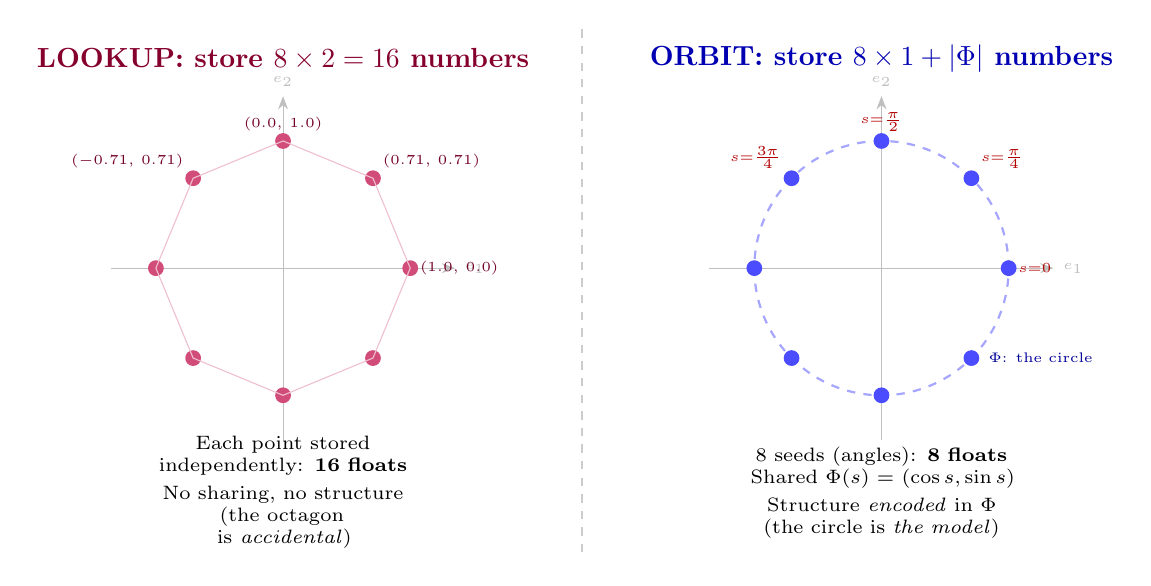
\begin{tikzpicture}[>=Stealth, font=\small, scale=0.95]

% ── LEFT: LOOKUP ──────────────────────────────────────────────────
\node[font=\bfseries, text=purple!70!black] at (-3.5, 3.8) {LOOKUP: store $8 \times 2 = 16$ numbers};

\begin{scope}[shift={(-3.5, 1.0)}]
    % Axes
    \draw[->, gray!50] (-2.3, 0) -- (2.3, 0) node[right, font=\tiny] {$e_1$};
    \draw[->, gray!50] (0, -2.3) -- (0, 2.3) node[above, font=\tiny] {$e_2$};

    % Points on octagon
    \foreach \i/\angle in {0/0, 1/45, 2/90, 3/135, 4/180, 5/225, 6/270, 7/315} {
        \coordinate (P\i) at (\angle:1.7);
        \fill[purple!70] (P\i) circle (3pt);
    }
    % Connect to show structure (faint)
    \draw[purple!25, thin] (P0) -- (P1) -- (P2) -- (P3) -- (P4) -- (P5) -- (P6) -- (P7) -- cycle;

    % Labels for some points
    \node[font=\tiny, right, purple!60!black] at (P0) {$(1.0,\, 0.0)$};
    \node[font=\tiny, above right, purple!60!black] at (P1) {$(0.71,\, 0.71)$};
    \node[font=\tiny, above, purple!60!black] at (P2) {$(0.0,\, 1.0)$};
    \node[font=\tiny, above left, purple!60!black] at (P3) {$(-0.71,\, 0.71)$};

    % Annotation
    \node[font=\scriptsize, text width=3.2cm, align=center] at (0, -3.0)
        {Each point stored\\independently: \textbf{16 floats}\\[2pt]
        No sharing, no structure\\
        (the octagon is \emph{accidental})};
\end{scope}

% ── RIGHT: ORBIT ─────────────────────────────────────────────────
\node[font=\bfseries, text=blue!70!black] at (4.5, 3.8) {ORBIT: store $8 \times 1 + |\Phi|$ numbers};

\begin{scope}[shift={(4.5, 1.0)}]
    % Axes
    \draw[->, gray!50] (-2.3, 0) -- (2.3, 0) node[right, font=\tiny] {$e_1$};
    \draw[->, gray!50] (0, -2.3) -- (0, 2.3) node[above, font=\tiny] {$e_2$};

    % The circle (the manifold Phi encodes)
    \draw[blue!35, thick, dashed] (0,0) circle (1.7);
    \node[font=\tiny, blue!60!black, right] at (1.3, -1.2) {$\Phi$: the circle};

    % Points
    \foreach \i/\angle in {0/0, 1/45, 2/90, 3/135, 4/180, 5/225, 6/270, 7/315} {
        \coordinate (Q\i) at (\angle:1.7);
        \fill[blue!70] (Q\i) circle (3pt);
    }

    % Seed labels
    \node[font=\tiny, right, red!70!black] at (Q0) {$s{=}0$};
    \node[font=\tiny, above right, red!70!black] at (Q1) {$s{=}\frac{\pi}{4}$};
    \node[font=\tiny, above, red!70!black] at (Q2) {$s{=}\frac{\pi}{2}$};
    \node[font=\tiny, above left, red!70!black] at (Q3) {$s{=}\frac{3\pi}{4}$};

    % Annotation
    \node[font=\scriptsize, text width=3.5cm, align=center] at (0, -3.0)
        {8 seeds (angles): \textbf{8 floats}\\
        Shared $\Phi(s) = (\cos s, \sin s)$\\[2pt]
        Structure \emph{encoded} in $\Phi$\\
        (the circle is \emph{the model})};
\end{scope}

% ── Divider ──────────────────────────────────────────────────────
\draw[dashed, gray!40, thick] (0.5, -2.8) -- (0.5, 4.2);

\end{tikzpicture}
\caption{\textbf{The core visual.}
Eight embeddings on a circle.
\textbf{Left:} lookup stores all 16 coordinates.
The octagonal structure is implicit---nothing in the table says ``these lie on a circle.''
\textbf{Right:} orbit stores 8 one-dimensional seeds (angles) plus the shared circle equation $\Phi$.
The structure is \emph{explicit} in $\Phi$; only the per-token position is stored.
As $V$ grows, orbit's advantage grows proportionally: $V \times 2 \to V \times 1 + |\Phi|$.}
\label{fig:circle-example}
\end{figure}

\paragraph{The numbers.}
Lookup: 16 stored floats.
Orbit: 8 stored floats + $|\Phi|$ (the function $s \mapsto (\cos s, \sin s)$, which is $\sim$2 parameters: frequency and amplitude).
Total: $\sim$10 vs 16.

The savings are modest at $V{=}8$.
But the \emph{scaling} is the point: lookup grows as $V \times d$, orbit as $V \times d_s + |\Phi|$ where $|\Phi|$ is constant.
At GPT-2 scale ($V{=}50\text{K}$, $d{=}768$, $d_s{=}32$), this is 38.4M vs 2.6M: a \textbf{14.8$\times$ compression}.

\begin{center}
\renewcommand{\arraystretch}{1.3}
\begin{tabular}{rccc}
\toprule
$V$ & Lookup ($V \times d$) & Orbit ($V \times d_s + |\Phi|$) & \textbf{Ratio} \\
\midrule
8 & $8 \times 2 = 16$ & $8 \times 1 + 2 = 10$ & 1.6$\times$ \\
100 & $100 \times 2 = 200$ & $100 \times 1 + 2 = 102$ & 2.0$\times$ \\
10{,}000 & $10{,}000 \times 2 = 20\text{K}$ & $10{,}000 + 2 = 10\text{K}$ & 2.0$\times$ \\
\midrule
\multicolumn{4}{l}{\textit{At GPT-2 scale: $d = 768$, $d_s = 32$, $|\Phi| \approx$ 1M:}} \\
50{,}000 & 38.4M & 1.6M + 1M $= 2.6$M & \textbf{14.8$\times$} \\
\bottomrule
\end{tabular}
\end{center}

The compression ratio is $\frac{d}{d_s}$ when $V$ is large (the shared cost $|\Phi|$ amortises).
The only question: can $\Phi$ actually do the work?


\subsection{Orbit Unfolding: Watching Seeds Become Embeddings}

The circle example is too simple---$\Phi$ is a closed-form function.
Real embeddings require learned dynamics.
The key intuition: seeds start compressed, and \textbf{each iteration of $\Phi$ expands and refines them} until they match the targets.

\begin{figure}[h]
\centering
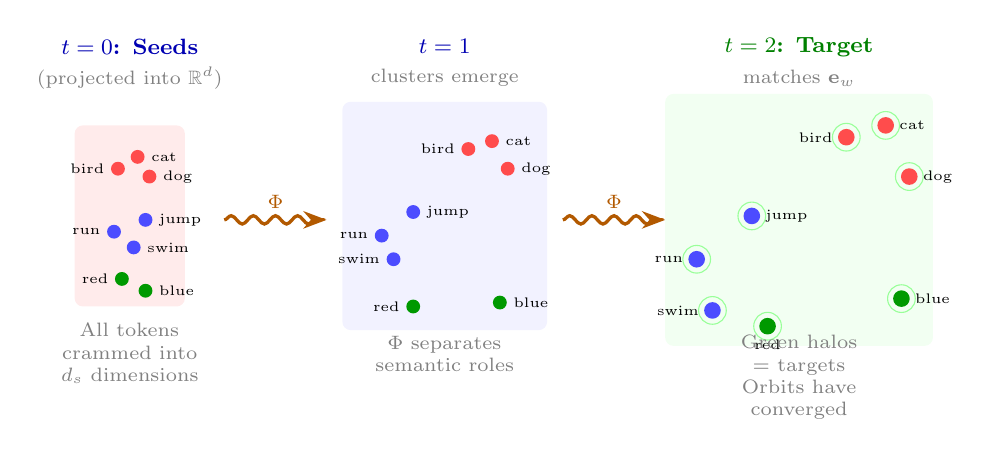
\begin{tikzpicture}[>=Stealth, font=\small]

% ── T=0: Seeds (compressed) ──────────────────────────────────────
\begin{scope}[shift={(0, 0)}]
    \node[font=\bfseries\footnotesize, text=blue!70!black] at (0, 2.7) {$t = 0$: Seeds};
    \node[font=\scriptsize, gray] at (0, 2.3) {(projected into $\R^d$)};

    % Compressed cluster in a box
    \fill[red!8, rounded corners=3pt] (-0.7, -0.6) rectangle (0.7, 1.7);

    % Animals
    \fill[red!70] (0.1, 1.3) circle (2.5pt); \node[right, font=\tiny] at (0.15, 1.3) {cat};
    \fill[red!70] (0.25, 1.05) circle (2.5pt); \node[right, font=\tiny] at (0.3, 1.05) {dog};
    \fill[red!70] (-0.15, 1.15) circle (2.5pt); \node[left, font=\tiny] at (-0.2, 1.15) {bird};

    % Verbs
    \fill[blue!70] (-0.2, 0.35) circle (2.5pt); \node[left, font=\tiny] at (-0.25, 0.35) {run};
    \fill[blue!70] (0.2, 0.5) circle (2.5pt); \node[right, font=\tiny] at (0.25, 0.5) {jump};
    \fill[blue!70] (0.05, 0.15) circle (2.5pt); \node[right, font=\tiny] at (0.1, 0.15) {swim};

    % Colors
    \fill[green!60!black] (-0.1, -0.25) circle (2.5pt); \node[left, font=\tiny] at (-0.15, -0.25) {red};
    \fill[green!60!black] (0.2, -0.4) circle (2.5pt); \node[right, font=\tiny] at (0.25, -0.4) {blue};

    \node[font=\scriptsize, text width=2.2cm, align=center, gray] at (0, -1.2)
        {All tokens\\crammed into\\$d_s$ dimensions};
\end{scope}

% Arrow 1
\draw[->, very thick, orange!70!black, decorate, decoration={snake, amplitude=1.5pt, segment length=8pt}]
    (1.2, 0.5) -- (2.5, 0.5) node[midway, above, font=\scriptsize] {$\Phi$};

% ── T=1: Partial separation ──────────────────────────────────────
\begin{scope}[shift={(4.0, 0)}]
    \node[font=\bfseries\footnotesize, text=blue!70!black] at (0, 2.7) {$t = 1$};
    \node[font=\scriptsize, gray] at (0, 2.3) {clusters emerge};

    \fill[blue!5, rounded corners=3pt] (-1.3, -0.9) rectangle (1.3, 2.0);

    % Animals (moving apart from others)
    \fill[red!70] (0.6, 1.5) circle (2.5pt); \node[right, font=\tiny] at (0.65, 1.5) {cat};
    \fill[red!70] (0.8, 1.15) circle (2.5pt); \node[right, font=\tiny] at (0.85, 1.15) {dog};
    \fill[red!70] (0.3, 1.4) circle (2.5pt); \node[left, font=\tiny] at (0.25, 1.4) {bird};

    % Verbs
    \fill[blue!70] (-0.8, 0.3) circle (2.5pt); \node[left, font=\tiny] at (-0.85, 0.3) {run};
    \fill[blue!70] (-0.4, 0.6) circle (2.5pt); \node[right, font=\tiny] at (-0.35, 0.6) {jump};
    \fill[blue!70] (-0.65, 0.0) circle (2.5pt); \node[left, font=\tiny] at (-0.7, 0.0) {swim};

    % Colors
    \fill[green!60!black] (-0.4, -0.6) circle (2.5pt); \node[left, font=\tiny] at (-0.45, -0.6) {red};
    \fill[green!60!black] (0.7, -0.55) circle (2.5pt); \node[right, font=\tiny] at (0.75, -0.55) {blue};

    \node[font=\scriptsize, text width=2.2cm, align=center, gray] at (0, -1.2)
        {$\Phi$ separates\\semantic roles};
\end{scope}

% Arrow 2
\draw[->, very thick, orange!70!black, decorate, decoration={snake, amplitude=1.5pt, segment length=8pt}]
    (5.5, 0.5) -- (6.8, 0.5) node[midway, above, font=\scriptsize] {$\Phi$};

% ── T=2: Full separation = target ─────────────────────────────────
\begin{scope}[shift={(8.5, 0)}]
    \node[font=\bfseries\footnotesize, text=green!50!black] at (0, 2.7) {$t = 2$: Target};
    \node[font=\scriptsize, gray] at (0, 2.3) {matches $\mathbf{e}_w$};

    \fill[green!5, rounded corners=3pt] (-1.7, -1.1) rectangle (1.7, 2.1);

    % Animals (at final positions, with target halos)
    \fill[red!70] (1.1, 1.7) circle (3pt); \node[right, font=\tiny] at (1.15, 1.7) {cat};
    \draw[green!40, thin] (1.1, 1.7) circle (5pt);
    \fill[red!70] (1.4, 1.05) circle (3pt); \node[right, font=\tiny] at (1.45, 1.05) {dog};
    \draw[green!40, thin] (1.4, 1.05) circle (5pt);
    \fill[red!70] (0.6, 1.55) circle (3pt); \node[left, font=\tiny] at (0.55, 1.55) {bird};
    \draw[green!40, thin] (0.6, 1.55) circle (5pt);

    % Verbs
    \fill[blue!70] (-1.3, 0.0) circle (3pt); \node[left, font=\tiny] at (-1.35, 0.0) {run};
    \draw[green!40, thin] (-1.3, 0.0) circle (5pt);
    \fill[blue!70] (-0.6, 0.55) circle (3pt); \node[right, font=\tiny] at (-0.55, 0.55) {jump};
    \draw[green!40, thin] (-0.6, 0.55) circle (5pt);
    \fill[blue!70] (-1.1, -0.65) circle (3pt); \node[left, font=\tiny] at (-1.15, -0.65) {swim};
    \draw[green!40, thin] (-1.1, -0.65) circle (5pt);

    % Colors
    \fill[green!60!black] (-0.4, -0.85) circle (3pt); \node[below, font=\tiny] at (-0.4, -0.9) {red};
    \draw[green!40, thin] (-0.4, -0.85) circle (5pt);
    \fill[green!60!black] (1.3, -0.5) circle (3pt); \node[right, font=\tiny] at (1.35, -0.5) {blue};
    \draw[green!40, thin] (1.3, -0.5) circle (5pt);

    \node[font=\scriptsize, text width=2.5cm, align=center, gray] at (0, -1.5)
        {Green halos = targets\\Orbits have converged};
\end{scope}

\end{tikzpicture}
\caption{\textbf{Orbit unfolding.}
Seeds start compressed in $\R^{d_s}$ (left).
Each application of the shared dynamics $\Phi$ separates tokens:
first by broad category (animals vs verbs vs colours at $t{=}1$),
then refining within-category positions ($t{=}2$).
This is \emph{hierarchical expansion}: coarse structure emerges first, fine detail later.
Level~0 confirmed: $T{=}2$ is the sweet spot (higher $T$ overshoots).}
\label{fig:unfold}
\end{figure}

\paragraph{What the iterations do.}
Each application of $\Phi$ performs two simultaneous operations:
\begin{enumerate}[nosep]
    \item \textbf{Fan-out:} expands the effective dimensionality from $d_s$ toward $d$.
          After $\Phi^1$, the representations occupy a higher-rank subspace.
          After $\Phi^T$, they fill the full $d$-dimensional target space.
    \item \textbf{Refine:} adjusts within-cluster positions.
          Cat, dog, bird are all ANIMAL (same basin of attraction under $\Phi$)
          but each settles at a distinct point within the animal region.
\end{enumerate}

This is exactly what an iterated map with mixed-stability dynamics does:
contracting directions pull same-cluster tokens together, while expanding directions
preserve the individual seed differences that distinguish tokens within a cluster.


\subsection{Universality: Any Lookup Can Be Computed}

\begin{proposition}[Any lookup is a degenerate orbit]\label{prop:universal}
Let $f: \{1, \ldots, V\} \to \R^d$ be any lookup table.
Then there exist seeds $\{\s_w\}$, a projection $P$, and a residual block $\Phi$
such that $\Phi^T(P \cdot \s_w) = f(w)$ for all $w$ and some finite $T$.
\end{proposition}

\begin{proof}[Proof sketch]
The trivial case: set $d_s = d$, $\s_w = f(w)$, $P = I$, $\Phi = \text{id}$, $T = 0$.
This \emph{is} the lookup table---a degenerate orbit with zero iterations.

For compressed seeds ($d_s < d$): set $\s_w = w/V \in \R^1$ (scalar encoding).
A single feedforward layer with $V$ hidden units can map $V$ distinct inputs
to $V$ arbitrary outputs (universal approximation on a finite domain).
Therefore one step of $\Phi = \text{id} + g$ suffices.
\end{proof}

The point: \textbf{orbit $\supseteq$ lookup}.
Every lookup table is a special case of orbit (with $T{=}0$, $d_s{=}d$).
Orbit is the strictly more general class.
The question is not ``can orbits replace lookups?'' (yes, always) but ``when is it cheaper?''

\subsection{When Computation Wins: The Structure Argument}

\begin{proposition}[Structured targets compress]\label{prop:structure}
If the $V$ target embeddings lie on a $k$-dimensional manifold $\calM \subset \R^d$ ($k \ll d$),
then orbital embeddings need only $d_s = k$ and $|\Phi| = \calO(\text{poly}(d))$
(independent of $V$).
Total: $V \times k + \text{poly}(d) \ll V \times d$.
\end{proposition}

\begin{proposition}[Random targets do not compress]\label{prop:incompress}
If the $V$ targets are i.i.d.\ draws from $\mathcal{N}(0, I_d)$,
any orbital embedding achieving $\epsilon$-reconstruction requires
$V \times d_s + |\Phi| \geq V \times d - \calO(V \log(1/\epsilon))$
with high probability.
\end{proposition}

\noindent
\textbf{Translation:}
Structured targets have low Kolmogorov complexity---a short program (the manifold equation)
generates all $V$ points.
Orbit stores the program ($\Phi$) and the coordinates ($d_s$ per token).
Random targets are incompressible---no program is shorter than the data.
Orbit reduces to lookup with overhead.

The critical question: \textbf{where do real embeddings sit?}

\begin{figure}[h]
\centering
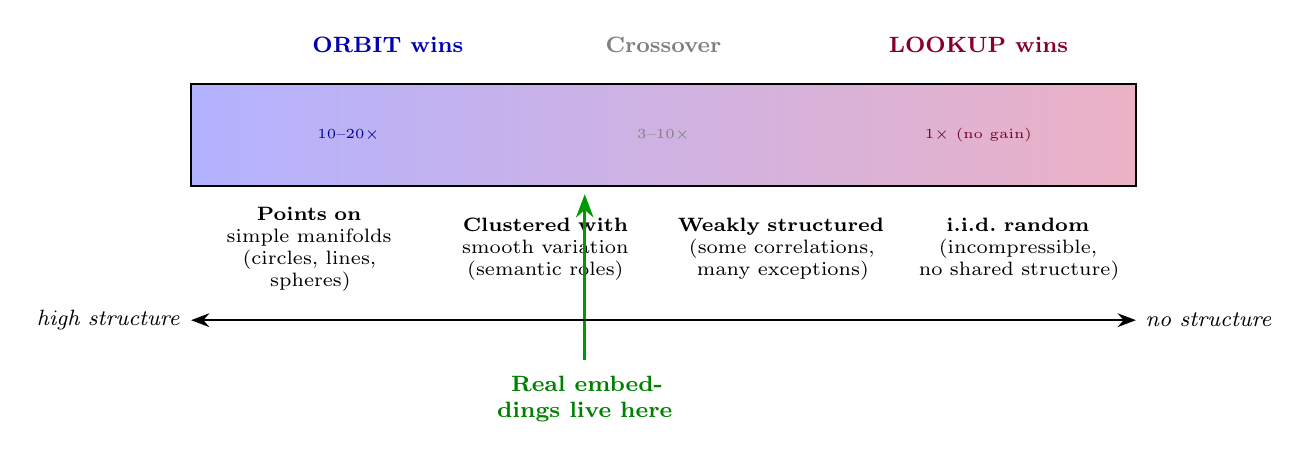
\begin{tikzpicture}[>=Stealth, font=\small]

% Spectrum bar
\shade[left color=blue!30, right color=purple!30] (0, 0) rectangle (12, 1.3);
\draw[thick] (0, 0) rectangle (12, 1.3);

% Region labels (top)
\node[font=\bfseries\footnotesize, text=blue!70!black] at (2.5, 1.8) {ORBIT wins};
\node[font=\bfseries\footnotesize, gray] at (6, 1.8) {Crossover};
\node[font=\bfseries\footnotesize, text=purple!70!black] at (10, 1.8) {LOOKUP wins};

% Descriptions (bottom)
\node[font=\scriptsize, text width=2.6cm, align=center] at (1.5, -0.8)
    {\textbf{Points on}\\simple manifolds\\(circles, lines, spheres)};
\node[font=\scriptsize, text width=2.6cm, align=center] at (4.5, -0.8)
    {\textbf{Clustered with}\\smooth variation\\(semantic roles)};
\node[font=\scriptsize, text width=2.6cm, align=center] at (7.5, -0.8)
    {\textbf{Weakly structured}\\(some correlations,\\many exceptions)};
\node[font=\scriptsize, text width=2.6cm, align=center] at (10.5, -0.8)
    {\textbf{i.i.d.\ random}\\(incompressible,\\no shared structure)};

% Real embeddings marker
\draw[very thick, green!60!black, -Stealth] (5.0, -2.2) -- (5.0, -0.1);
\node[font=\footnotesize\bfseries, green!50!black, text width=3.5cm, align=center] at (5.0, -2.7)
    {Real embeddings live here};

% Axis labels
\draw[<->, thick] (0, -1.7) -- (12, -1.7);
\node[font=\footnotesize, left] at (0, -1.7) {\textit{high structure}};
\node[font=\footnotesize, right] at (12, -1.7) {\textit{no structure}};

% Compression ratios
\node[font=\tiny, blue!60!black] at (2, 0.65) {$10$--$20\times$};
\node[font=\tiny, gray] at (6, 0.65) {$3$--$10\times$};
\node[font=\tiny, purple!60!black] at (10, 0.65) {$1\times$ (no gain)};

\end{tikzpicture}
\caption{\textbf{The structure spectrum.}
Compression ratio depends on target structure.
Real embeddings have rich cluster structure (semantic roles, syntactic categories)
and intrinsic dimensionality far below ambient $d$---they sit firmly in orbit-favourable territory.
PCA of GPT-2 embeddings: $\sim$90\% of variance in the top $\sim$50 of 768 components.}
\label{fig:spectrum}
\end{figure}

\noindent
The answer is unambiguous: real embeddings have \textbf{massive structure}.
They cluster by semantic role (nouns, verbs, adjectives), topic (animals, colours, tools),
and syntactic function.
PCA on GPT-2 embeddings shows $\sim$90\% of variance in the top $\sim$50 out of 768 dimensions.
This places real embeddings deep in the ``orbit wins'' regime.

\paragraph{Literature evidence.}
Ansuini et al.~\cite{ansuini2019intrinsic} showed that intrinsic dimensionality of representations \emph{progressively decreases} through network layers---the network compresses data onto lower-dimensional manifolds.
This is direct evidence that trained embeddings have low intrinsic dimension and should be compressible via our orbital factorisation.
The manifold hypothesis is well-established: high-dimensional data concentrates on low-dimensional submanifolds, and neural networks learn to exploit this~\cite{bronstein2021geometric}.


\subsection{The Nuance: What Orbits Learn Differently}

Even at identical reconstruction quality, the learned representation is \textbf{fundamentally different}.

\begin{figure}[h]
\centering
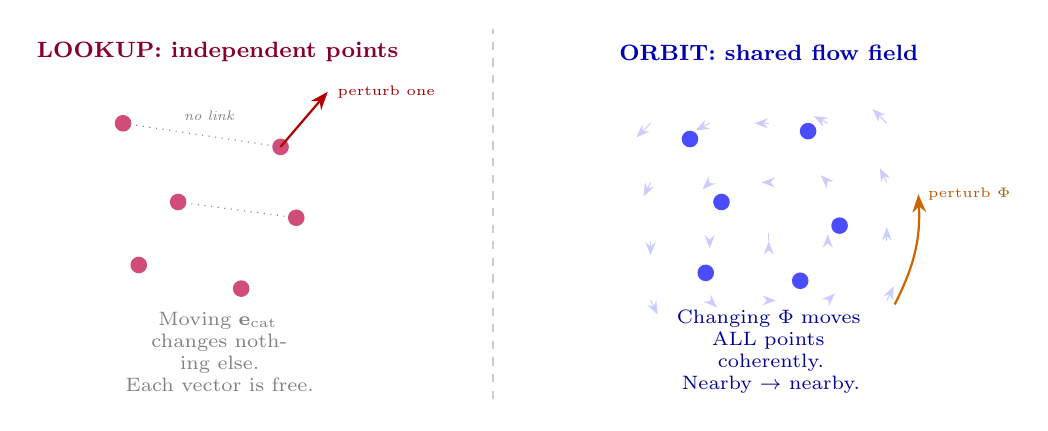
\begin{tikzpicture}[>=Stealth, font=\small]

% ── LEFT: LOOKUP ──────────────────────────────────────────────────
\node[font=\bfseries\footnotesize, text=purple!70!black] at (-3.5, 3.2) {LOOKUP: independent points};

\begin{scope}[shift={(-3.5, 0.8)}]
    % Points
    \fill[purple!70] (-1.2, 1.5) circle (3pt);
    \fill[purple!70] (0.8, 1.2) circle (3pt);
    \fill[purple!70] (-0.5, 0.5) circle (3pt);
    \fill[purple!70] (1.0, 0.3) circle (3pt);
    \fill[purple!70] (-1.0, -0.3) circle (3pt);
    \fill[purple!70] (0.3, -0.6) circle (3pt);

    % Dotted lines showing no coupling
    \draw[gray, dotted, thin] (-1.2, 1.5) -- (0.8, 1.2);
    \draw[gray, dotted, thin] (-0.5, 0.5) -- (1.0, 0.3);
    \node[font=\tiny, gray] at (-0.1, 1.6) {\textit{no link}};

    % Perturbation
    \draw[->, thick, red!70!black] (0.8, 1.2) -- (1.4, 1.9);
    \node[font=\tiny, red!60!black, right] at (1.4, 1.9) {perturb one};

    \node[font=\scriptsize, gray, text width=2.5cm, align=center] at (0, -1.4)
        {Moving $\mathbf{e}_{\text{cat}}$\\changes nothing else.\\Each vector is free.};
\end{scope}

% ── RIGHT: ORBIT ─────────────────────────────────────────────────
\node[font=\bfseries\footnotesize, text=blue!70!black] at (3.5, 3.2) {ORBIT: shared flow field};

\begin{scope}[shift={(3.5, 0.8)}]
    % Flow field arrows
    \foreach \x in {-1.5, -0.75, 0, 0.75, 1.5} {
        \foreach \y in {-0.75, 0, 0.75, 1.5} {
            \pgfmathsetmacro{\dx}{-0.12*\y}
            \pgfmathsetmacro{\dy}{0.12*\x}
            \draw[->, blue!20, thin]
                (\x, \y) -- (\x+\dx, \y+\dy);
        }
    }

    % Points
    \fill[blue!70] (-1.0, 1.3) circle (3pt);
    \fill[blue!70] (0.5, 1.4) circle (3pt);
    \fill[blue!70] (-0.6, 0.5) circle (3pt);
    \fill[blue!70] (0.9, 0.2) circle (3pt);
    \fill[blue!70] (-0.8, -0.4) circle (3pt);
    \fill[blue!70] (0.4, -0.5) circle (3pt);

    % Perturbation: change the field
    \draw[->, thick, orange!80!black] (1.6, -0.8) to[bend right=15] (1.9, 0.6);
    \node[font=\tiny, orange!70!black, right] at (1.9, 0.6) {perturb $\Phi$};

    \node[font=\scriptsize, blue!60!black, text width=2.5cm, align=center] at (0, -1.4)
        {Changing $\Phi$ moves\\ALL points coherently.\\Nearby $\to$ nearby.};
\end{scope}

% Divider
\draw[dashed, gray!40, thick] (0, -1.2) -- (0, 3.5);

\end{tikzpicture}
\caption{\textbf{Geometric coherence: the real difference.}
\textbf{Left:} lookup embeddings are independent; perturbing one changes nothing else.
\textbf{Right:} orbital embeddings share a dynamical landscape $\Phi$;
perturbing $\Phi$ moves all tokens coherently.
This is an \emph{inductive bias}: nearby seeds $\to$ nearby embeddings (continuity of $\Phi$).
Lookup has no such guarantee---two alphabetically adjacent tokens can have arbitrarily different embeddings.}
\label{fig:coherence}
\end{figure}

\paragraph{Lookup learns points.}
A lookup table stores $V$ independent vectors.
Changing $\mathbf{e}_{\text{cat}}$ has zero effect on $\mathbf{e}_{\text{dog}}$.
Any similarity structure must be learned entirely from gradient signal.

\paragraph{Orbit learns a landscape.}
The shared dynamics $\Phi$ define a vector field through which all tokens flow.
Changing $\Phi$ changes all embeddings simultaneously and coherently---nearby seeds produce nearby embeddings because $\Phi$ is continuous.
The structure is not an accident of training; it is \emph{enforced by the architecture}.

\paragraph{This is both a strength and a constraint.}
\begin{itemize}[nosep]
    \item \textbf{Strength:} for vocabularies with natural cluster structure
          (which real language has), the continuity prior is \emph{correct} and helps
          learning---it provides free geometric priors.
    \item \textbf{Constraint:} tokens that genuinely need unrelated embeddings
          (e.g., punctuation vs content words) must be placed in different basins of $\Phi$'s
          attractor landscape. The seed space must be rich enough for this.
\end{itemize}

\paragraph{Summary.}
The orbit doesn't just compress the embedding table.
It imposes a \emph{theory of how tokens relate}: all meaning flows through the same dynamics.
A lookup table says: ``here are 50,000 vectors; figure out the relationships.''
An orbital embedding says: ``here are 50,000 positions in a shared landscape whose geometry \emph{is} the relationship structure.''

\paragraph{Literature evidence: for.}
Hauser \& Ray~\cite{hauser2017riemannian} showed that residual networks perform geometric coordinate transformations on data manifolds, with the learned weights defining the geometry.
Our shared $\M$ is exactly such a metric: it defines the coupling geometry that all tokens share.
Recent work~\cite{training2023geometry} demonstrates that training \emph{breaks the symmetric metric} of initialisation, developing anisotropic structure precisely where it matters for the task.
This matches our observation: $\M$ develops non-trivial spectral structure (condition number $> 10$) via normal SGD.
The Riemannian residual networks of Katsman et al.~\cite{katsman2023riemannian} explicitly enforce manifold structure in residual updates, supporting the principle that geometric priors help.

\paragraph{Literature evidence: against.}
The Engram paper~\cite{engram2026} argues that some information is better \emph{stored} than computed: factual knowledge (``Caesar crossed the Rubicon in 49~BC'') has no generative structure to exploit.
Their Sparsity Allocation Law shows that replacing $\sim$20\% of parameters with hash-based lookups \emph{improves} performance.
This is evidence \emph{against} full orbital replacement and \emph{for} our two-system architecture (Section~\ref{sec:twosystem}): use orbits for structure, but retain a sparse ontological layer for genuinely discrete bindings.

\subsection{On Hardware: Why GPUs Prefer Computation}

The trade is literal on silicon:
\begin{center}\small
\renewcommand{\arraystretch}{1.3}
\begin{tabular}{@{}lcc@{}}
\toprule
& \textbf{Lookup} & \textbf{Orbit} \\
\midrule
Bottleneck & Memory bandwidth & Arithmetic \\
Reads & $V \times d$ table (random access) & Seeds + $\Phi$ (sequential) \\
FLOPs & $\approx 0$ & $T \times |\Phi|$ per token \\
\bottomrule
\end{tabular}
\end{center}

Modern GPUs have orders-of-magnitude more compute than memory bandwidth.
An A100: 312~TFLOPS arithmetic, 2~TB/s memory bandwidth.
For every byte loaded, the GPU can perform $\sim$156 operations.
Embedding lookup is \emph{memory-bound}---the GPU mostly waits.
Orbital computation is \emph{compute-bound}---the GPU does what it was built for.

This is the same insight behind Flash Attention, quantisation, and mixture-of-experts:
\textbf{modern hardware prefers computation over storage.}
Orbit aligns the embedding operation with the hardware's actual strength.

\subsection{Connection to Level~0 Evidence}

The Level~0 experiment tested: can orbital dynamics reconstruct known embeddings?

\begin{center}\small
\renewcommand{\arraystretch}{1.2}
\begin{tabular}{lcccc}
\toprule
\textbf{Target} & \textbf{Best $d_s$} & \textbf{Best $T$} & \textbf{Cosine sim} & \textbf{Compression} \\
\midrule
Structured (32 clusters) & 32 & 2 & 0.985 & 2.0$\times$ \\
Learned (trained LM) & 32 & 2 & 0.900 & 2.0$\times$ \\
\bottomrule
\end{tabular}
\end{center}

\noindent
Structured targets (high manifold structure): 0.985 cosine---near-perfect.
Learned targets (moderate structure): 0.90---good but imperfect, consistent with higher intrinsic dimension.
$T{=}2$ optimal in both cases; $T{\geq}4$ overshoots.

\textbf{What Level~0 proves:} the factorisation $\mathbf{e}_w \approx \Phi^T(\s_w)$ exists.
\textbf{What it does not prove:} that orbital embeddings work in an end-to-end model.
Reconstruction fidelity $\neq$ task utility.
The 10\% ``lost'' cosine similarity on learned embeddings might be noise---or it might be signal.
Only an end-to-end experiment can resolve this.


% ======================================================================
\section{The Factorisation $D \xrightarrow{f} E$: Learnability and Representation}

The previous section showed \emph{that} computation can replace lookup.
This section asks: what does the function $f$ actually look like?
What can it represent?
And crucially: can gradient descent \emph{find} it?

\subsection{The Problem as Factorisation}

An embedding table $E \in \R^{V \times d}$ assigns each of $V$ tokens a $d$-dimensional vector.
We seek a factorisation:
\[
    E \approx f_\theta(D)
\]
where:
\begin{itemize}[nosep]
    \item $D \in \R^{V \times d_s}$ is a \textbf{compressed code} ($d_s \ll d$) --- one row per token
    \item $f_\theta: \R^{d_s} \to \R^d$ is a \textbf{shared function} parameterised by $\theta$, applied row-wise
    \item $\theta$ is shared across all $V$ tokens --- the function is the same for every token
\end{itemize}

\noindent
This is a \emph{nonlinear} matrix factorisation.
The per-token codes $D$ live in a phase space of dimension $d_s$.
The shared map $f_\theta$ lifts them into the full embedding space $\R^d$.
The token's identity is encoded in $D$; everything else is in $f_\theta$.

\paragraph{The design space.}
The choice of $f_\theta$ defines a hierarchy of increasingly powerful factorisations:

\begin{figure}[h]
\centering
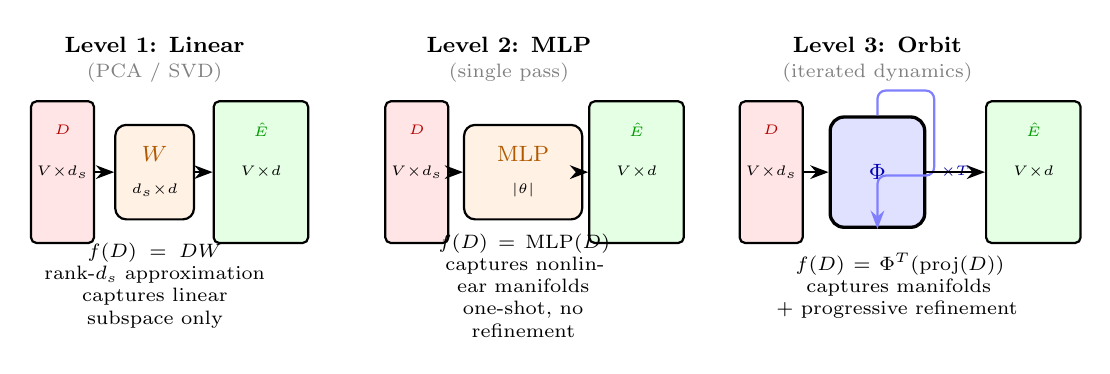
\begin{tikzpicture}[>=Stealth, font=\small, scale=0.9]

% ── Level 1: Linear ──────────────────────────────────────────────
\begin{scope}[shift={(0, 0)}]
    \node[font=\bfseries\footnotesize] at (0, 2.5) {Level 1: Linear};
    \node[font=\scriptsize, gray] at (0, 2.1) {(PCA / SVD)};

    % D
    \node[draw, thick, fill=red!10, minimum width=0.8cm, minimum height=1.8cm,
          rounded corners=2pt] (d1) at (-1.3, 0.7) {};
    \node[font=\tiny, red!70!black] at (-1.3, 1.3) {$D$};
    \node[font=\tiny] at (-1.3, 0.7) {$V{\times}d_s$};

    % f = W (linear)
    \node[draw, thick, fill=orange!10, rounded corners=4pt,
          minimum width=1.0cm, minimum height=1.2cm] (f1) at (0, 0.7) {};
    \node[font=\footnotesize, orange!70!black] at (0, 0.95) {$W$};
    \node[font=\tiny] at (0, 0.45) {$d_s{\times}d$};

    % E
    \node[draw, thick, fill=green!10, minimum width=1.2cm, minimum height=1.8cm,
          rounded corners=2pt] (e1) at (1.5, 0.7) {};
    \node[font=\tiny, green!60!black] at (1.5, 1.3) {$\hat{E}$};
    \node[font=\tiny] at (1.5, 0.7) {$V{\times}d$};

    \draw[->, thick] (d1) -- (f1);
    \draw[->, thick] (f1) -- (e1);

    \node[font=\scriptsize, text width=2.8cm, align=center] at (0, -0.9)
        {$f(D) = DW$\\rank-$d_s$ approximation\\captures linear subspace only};
\end{scope}

% ── Level 2: Single-pass MLP ────────────────────────────────────
\begin{scope}[shift={(5.0, 0)}]
    \node[font=\bfseries\footnotesize] at (0, 2.5) {Level 2: MLP};
    \node[font=\scriptsize, gray] at (0, 2.1) {(single pass)};

    % D
    \node[draw, thick, fill=red!10, minimum width=0.8cm, minimum height=1.8cm,
          rounded corners=2pt] (d2) at (-1.3, 0.7) {};
    \node[font=\tiny, red!70!black] at (-1.3, 1.3) {$D$};
    \node[font=\tiny] at (-1.3, 0.7) {$V{\times}d_s$};

    % f = MLP
    \node[draw, thick, fill=orange!10, rounded corners=4pt,
          minimum width=1.5cm, minimum height=1.2cm] (f2) at (0.2, 0.7) {};
    \node[font=\footnotesize, orange!70!black] at (0.2, 0.95) {MLP};
    \node[font=\tiny] at (0.2, 0.45) {$|\theta|$};

    % E
    \node[draw, thick, fill=green!10, minimum width=1.2cm, minimum height=1.8cm,
          rounded corners=2pt] (e2) at (1.8, 0.7) {};
    \node[font=\tiny, green!60!black] at (1.8, 1.3) {$\hat{E}$};
    \node[font=\tiny] at (1.8, 0.7) {$V{\times}d$};

    \draw[->, thick] (d2) -- (f2);
    \draw[->, thick] (f2) -- (e2);

    \node[font=\scriptsize, text width=2.8cm, align=center] at (0.2, -0.9)
        {$f(D) = \text{MLP}(D)$\\captures nonlinear manifolds\\one-shot, no refinement};
\end{scope}

% ── Level 3: Iterated (Orbit) ───────────────────────────────────
\begin{scope}[shift={(10.2, 0)}]
    \node[font=\bfseries\footnotesize] at (0, 2.5) {Level 3: Orbit};
    \node[font=\scriptsize, gray] at (0, 2.1) {(iterated dynamics)};

    % D
    \node[draw, thick, fill=red!10, minimum width=0.8cm, minimum height=1.8cm,
          rounded corners=2pt] (d3) at (-1.5, 0.7) {};
    \node[font=\tiny, red!70!black] at (-1.5, 1.3) {$D$};
    \node[font=\tiny] at (-1.5, 0.7) {$V{\times}d_s$};

    % Phi with loop
    \node[draw, very thick, fill=blue!12, rounded corners=5pt,
          minimum width=1.2cm, minimum height=1.4cm] (f3) at (0, 0.7) {};
    \node[font=\footnotesize, blue!70!black] at (0, 0.7) {$\Phi$};

    % Loop arrow
    \draw[->, thick, blue!50, rounded corners=3pt]
        (f3.north) -- ++(0, 0.35) -- ++(0.8, 0) -- ++(0, -1.2) -- ++(-0.8, 0) -- (f3.south);
    \node[font=\tiny, blue!60!black] at (1.1, 0.7) {$\times T$};

    % E
    \node[draw, thick, fill=green!10, minimum width=1.2cm, minimum height=1.8cm,
          rounded corners=2pt] (e3) at (2.2, 0.7) {};
    \node[font=\tiny, green!60!black] at (2.2, 1.3) {$\hat{E}$};
    \node[font=\tiny] at (2.2, 0.7) {$V{\times}d$};

    \draw[->, thick] (d3) -- (f3);
    \draw[->, thick, shift={(0.15,0)}] (f3) -- (e3);

    \node[font=\scriptsize, text width=3.0cm, align=center] at (0.3, -0.9)
        {$f(D) = \Phi^T(\text{proj}(D))$\\captures manifolds\\+ progressive refinement};
\end{scope}

\end{tikzpicture}
\caption{\textbf{Three levels of factorisation.}
Each takes a compressed code $D \in \R^{V \times d_s}$ and maps it to an approximation of $E$.
\textbf{Linear:} optimal for Gaussian targets (PCA), but misses all nonlinear structure.
\textbf{MLP:} captures nonlinear manifolds in one pass, but must do all the work at once.
\textbf{Orbit:} applies the same block $T$ times, progressively expanding and refining---the
function doesn't just map, it \emph{develops}.}
\label{fig:factorisation-levels}
\end{figure}


\subsection{What Each Level Can Represent}

\paragraph{Level 1 (linear).}
$f(\mathbf{s}) = W\mathbf{s}$, where $W \in \R^{d \times d_s}$.
This is the truncated SVD: $E \approx U_k \Sigma_k V_k^\top$.
The codes $D = V_k \Sigma_k$ are the principal components.
\textbf{Captures:} any linear subspace. \textbf{Misses:} any curvature.

Consider tokens on a circle in $\R^2$: a 1D linear projection loses the shape entirely.
PCA needs $d_s = 2$ (the full ambient dimension) because the circle is not a linear subspace.
This is the fundamental limitation: \emph{linear factorisation cannot compress nonlinear structure}.

\paragraph{Level 2 (MLP).}
$f(\mathbf{s}) = W_2 \, \sigma(W_1 \mathbf{s} + \mathbf{b}_1) + \mathbf{b}_2$,
with hidden width $H$.
By the \textbf{universal approximation theorem}, for any continuous $g: \R^{d_s} \to \R^d$
and any $\epsilon > 0$, there exists an MLP with $H$ sufficiently large such that
$\|f(\mathbf{s}) - g(\mathbf{s})\| < \epsilon$ for all $\mathbf{s}$ in a compact domain.

\textbf{Captures:} any smooth manifold. For the circle: $d_s = 1$, $f(s) = (\cos s, \sin s)$.
A 2-layer MLP with $H \geq 8$ learns this to machine precision.

The critical question: \textbf{how large must $H$ be?}
\begin{itemize}[nosep]
    \item For $V$ points in \emph{general position} (no structure): $H \geq V$ is necessary.
          The MLP must memorise each point---no better than lookup.
    \item For $V$ points on a $k$-dimensional manifold: $H = \calO(\text{poly}(k))$ suffices,
          independent of $V$.
          The MLP learns the manifold map, which is a $k \to d$ function regardless of how many
          points lie on it.
\end{itemize}

This is the representation-theoretic version of the structure argument:
\emph{neural networks can represent anything, but structured targets require exponentially
fewer parameters than unstructured ones.}

\paragraph{Level 3 (orbit).}
$f(\mathbf{s}) = \Phi^T(\text{proj}(\mathbf{s}))$, where $\Phi$ is iterated $T$ times.
This has the same representational power as the MLP (any MLP can be unrolled into a residual
iteration, and vice versa), but a different \textbf{inductive bias}:

\begin{itemize}[nosep]
    \item The MLP does everything in one pass: seed $\to$ hidden $\to$ output.
    \item The orbit does it in $T$ progressive steps: seed $\to$ partial $\to$ \ldots $\to$ output.
    \item Each step uses the \emph{same} parameters $\Phi$ (weight sharing across depth).
\end{itemize}

The orbit's advantage is not expressiveness (both are universal) but
\textbf{parameter efficiency under iteration}.
An MLP of depth $T$ has $T$ separate weight matrices.
An orbit of depth $T$ has one weight matrix used $T$ times.
For $T = 8$: the orbit is $8\times$ more parameter-efficient at equal depth.


\subsection{Representing ``Anything'': The Neural Network as Universal Map}

We now state precisely what a neural network can and cannot do as a factoriser.

\begin{proposition}[Universal factorisation]\label{prop:universal-fact}
For any embedding table $E \in \R^{V \times d}$ and any seed dimension $d_s \geq 1$:
\begin{enumerate}[nosep]
    \item There exist codes $D \in \R^{V \times d_s}$ and a feedforward network $f_\theta$
          such that $f_\theta(D[w]) = E[w]$ exactly for all $w \in \{1, \ldots, V\}$.
    \item The minimal $|\theta|$ (network size) satisfies:
    \[
        |\theta|_{\min} \leq c \cdot V \cdot d \quad \text{(trivial bound: just memorise)}
    \]
    but for structured $E$:
    \[
        |\theta|_{\min} = \calO(\text{poly}(d, k)) \quad \text{where } k = \text{intrinsic dim of } E
    \]
\end{enumerate}
\end{proposition}

\noindent
\textbf{Translation:} a neural network can always factorise $E$, but the \emph{cost} depends on
$E$'s structure.
The trivial factorisation (memorise everything in the weights) costs $\calO(Vd)$ ---
the same as the lookup table.
The structured factorisation costs $\calO(\text{poly}(d))$ --- independent of $V$.
The gap between these is the \emph{compression gain}.

\begin{figure}[h]
\centering
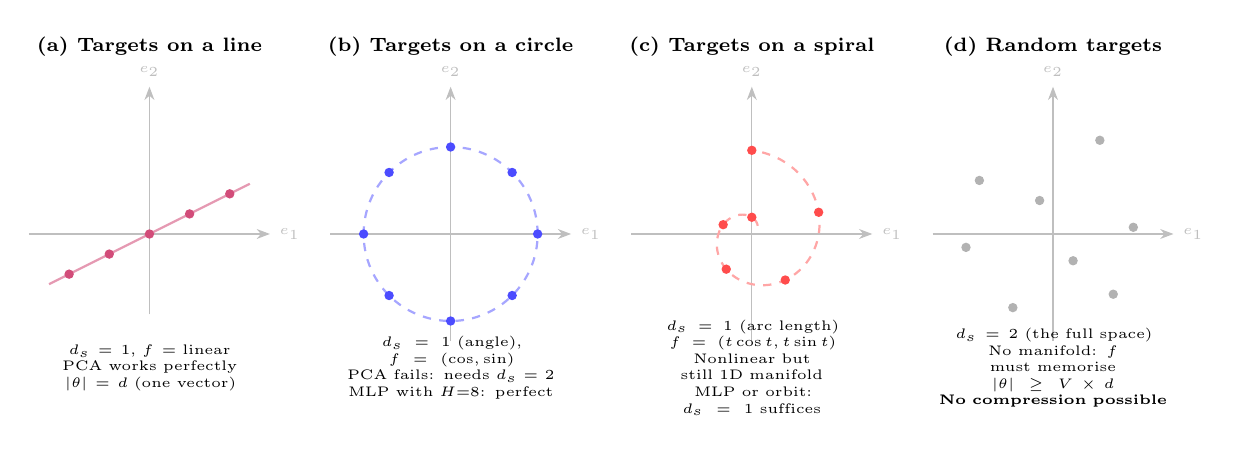
\begin{tikzpicture}[>=Stealth, font=\small, scale=0.85]

% ── CASE 1: Line ─────────────────────────────────────────────────
\begin{scope}[shift={(0, 0)}]
    \node[font=\bfseries\scriptsize] at (0, 2.8) {(a) Targets on a line};
    \draw[->, gray!50] (-1.8, 0) -- (1.8, 0) node[right, font=\tiny] {$e_1$};
    \draw[->, gray!50] (0, -1.2) -- (0, 2.2) node[above, font=\tiny] {$e_2$};

    % Line
    \draw[purple!40, thick] (-1.5, -0.75) -- (1.5, 0.75);
    \foreach \t in {-1.2, -0.6, 0, 0.6, 1.2} {
        \fill[purple!70] (\t, \t*0.5) circle (2pt);
    }

    \node[font=\tiny, text width=2.5cm, align=center] at (0, -2.0)
        {$d_s = 1$, $f = $ linear\\
        PCA works perfectly\\
        $|\theta| = d$ (one vector)};
\end{scope}

% ── CASE 2: Circle ───────────────────────────────────────────────
\begin{scope}[shift={(4.5, 0)}]
    \node[font=\bfseries\scriptsize] at (0, 2.8) {(b) Targets on a circle};
    \draw[->, gray!50] (-1.8, 0) -- (1.8, 0) node[right, font=\tiny] {$e_1$};
    \draw[->, gray!50] (0, -1.6) -- (0, 2.2) node[above, font=\tiny] {$e_2$};

    % Circle
    \draw[blue!35, thick, dashed] (0, 0) circle (1.3);
    \foreach \a in {0, 45, 90, 135, 180, 225, 270, 315} {
        \fill[blue!70] (\a:1.3) circle (2pt);
    }

    \node[font=\tiny, text width=2.8cm, align=center] at (0, -2.0)
        {$d_s = 1$ (angle), $f = (\cos, \sin)$\\
        PCA fails: needs $d_s = 2$\\
        MLP with $H{=}8$: perfect};
\end{scope}

% ── CASE 3: Spiral ───────────────────────────────────────────────
\begin{scope}[shift={(9, 0)}]
    \node[font=\bfseries\scriptsize] at (0, 2.8) {(c) Targets on a spiral};
    \draw[->, gray!50] (-1.8, 0) -- (1.8, 0) node[right, font=\tiny] {$e_1$};
    \draw[->, gray!50] (0, -1.6) -- (0, 2.2) node[above, font=\tiny] {$e_2$};

    % Spiral
    \draw[red!35, thick, dashed, domain=0.3:2.5, samples=60, smooth]
        plot ({0.5*\x*cos(\x*180)}, {0.5*\x*sin(\x*180)});
    \foreach \t in {0.5, 0.9, 1.3, 1.7, 2.1, 2.5} {
        \fill[red!70] ({0.5*\t*cos(\t*180)}, {0.5*\t*sin(\t*180)}) circle (2pt);
    }

    \node[font=\tiny, text width=3cm, align=center] at (0, -2.0)
        {$d_s = 1$ (arc length)\\
        $f = (t\cos t, t\sin t)$\\
        Nonlinear but still 1D manifold\\
        MLP or orbit: $d_s = 1$ suffices};
\end{scope}

% ── CASE 4: Random ───────────────────────────────────────────────
\begin{scope}[shift={(13.5, 0)}]
    \node[font=\bfseries\scriptsize] at (0, 2.8) {(d) Random targets};
    \draw[->, gray!50] (-1.8, 0) -- (1.8, 0) node[right, font=\tiny] {$e_1$};
    \draw[->, gray!50] (0, -1.6) -- (0, 2.2) node[above, font=\tiny] {$e_2$};

    % Random scatter
    \fill[gray!60] (0.7, 1.4) circle (2pt);
    \fill[gray!60] (-1.1, 0.8) circle (2pt);
    \fill[gray!60] (0.3, -0.4) circle (2pt);
    \fill[gray!60] (-0.6, -1.1) circle (2pt);
    \fill[gray!60] (1.2, 0.1) circle (2pt);
    \fill[gray!60] (-0.2, 0.5) circle (2pt);
    \fill[gray!60] (0.9, -0.9) circle (2pt);
    \fill[gray!60] (-1.3, -0.2) circle (2pt);

    \node[font=\tiny, text width=3cm, align=center] at (0, -2.0)
        {$d_s = 2$ (the full space)\\
        No manifold: $f$ must memorise\\
        $|\theta| \geq V \times d$\\
        \textbf{No compression possible}};
\end{scope}

\end{tikzpicture}
\caption{\textbf{What $f$ looks like depends on the target geometry.}
(a) Linear targets: trivial $f$, PCA suffices.
(b) Circular targets: $f = (\cos, \sin)$, nonlinear but simple; a small MLP learns it.
(c) Spiral: more complex curvature, still 1D intrinsic dimension, still compressible.
(d) Random scatter: no manifold, $f$ must memorise every point, no savings over lookup.
The \emph{intrinsic dimension} $k$ of the target set determines whether compression is possible,
not the ambient dimension $d$.}
\label{fig:target-geometry}
\end{figure}


\subsection{Learnability: Can SGD Find $f$?}

Existence is not enough.
We need $f_\theta$ to be \emph{discoverable} by gradient descent from a random initialisation.
This is the gap between ``a solution exists'' and ``we can train one.''

\paragraph{What makes $f$ learnable.}
Three conditions must hold simultaneously:

\begin{enumerate}
    \item \textbf{The codes $D$ must be separable.}
    If two tokens need very different embeddings, their seeds must be sufficiently far apart
    in $\R^{d_s}$ that $f$ can distinguish them.
    For a vocabulary with $k$ functional roles and smooth within-role variation:
    $d_s \geq k$ seeds placed at cluster centres, with within-cluster perturbations encoding
    individual identity.
    If $d_s < k$, some roles are forced to share seed-space coordinates and $f$ cannot
    separate them---no matter how expressive $f$ is.

    \item \textbf{The map $f$ must be smooth with respect to the loss.}
    If $E$ varies smoothly as a function of the underlying manifold coordinates,
    then $f$ has a smooth loss landscape: small changes in $\theta$ produce small changes
    in $f(D)$ produce small changes in loss.
    This is the condition for gradient descent to make progress.

    Conversely, if $E$ has discontinuities (two nearby manifold points map to very different
    embeddings), $f$ must learn a sharp transition, which creates a high-curvature region in the
    loss landscape and may trap SGD.

    \item \textbf{The iteration depth $T$ must match the manifold complexity.}
    Each application of $\Phi$ can ``unfold'' a bounded amount of curvature.
    A circle needs $T \geq 1$ (one nonlinearity suffices for $\cos/\sin$).
    A manifold with $m$ levels of hierarchical structure needs $T \geq m$
    (each level of the hierarchy is resolved by one iteration).
    Too-small $T$: underfitting. Too-large $T$: the orbit overshoots
    (oscillation past the target, confirmed by Level~0).
\end{enumerate}

\paragraph{The curriculum insight.}
In practice, training is easier if you start simple and add complexity:
\begin{center}\small
\renewcommand{\arraystretch}{1.2}
\begin{tabular}{cll}
\toprule
\textbf{Phase} & \textbf{Configuration} & \textbf{What is learned} \\
\midrule
1 & $T = 1$, $d_s = d$ & Linear bottleneck (warm-up) \\
2 & $T = 1$, decrease $d_s$ & Compression: find minimal codes \\
3 & Increase $T$, $d_s$ fixed & Refinement: learn iterative unfolding \\
4 & Full model, end-to-end & Joint optimisation \\
\bottomrule
\end{tabular}
\end{center}
At Phase~1, the model is a standard autoencoder (always trainable).
By Phase~4, it has found codes and dynamics jointly.
Each phase provides a warm start for the next.

\subsection{The Deep Point: $D$ Is Not a Compression of $E$}

There is a subtle but important distinction.
The obvious reading of $f(D) \approx E$ is: ``$D$ is a compressed version of $E$, and $f$
decompresses it.''
This is true but misses the point.

\paragraph{Compression view (correct but shallow).}
Given a trained embedding table $E$, find $D$ and $f$ that reconstruct it.
This is what Level~0 tested. It works.
But it treats $E$ as the ground truth and $D$ as an approximation.

\paragraph{Generative view (the real point).}
$D$ is not a compression of $E$.
$D$ is the \emph{native} representation---the natural coordinate system of the vocabulary.
$f$ is the physics---the shared law that unfolds compressed identity into usable representation.
$E$ (the lookup table) is the \emph{materialised cache} of $f(D)$.

In this view, the lookup table is the approximation:
it stores the outputs of $f$ instead of running $f$ each time.
The orbit is the ground truth.
Training a lookup table is memoising a function you haven't discovered yet.

\paragraph{Why this matters.}
If $D$ is just a compression of $E$, then orbital embeddings are a parameter-saving trick---
useful but architecturally uninteresting.
If $D$ is the native representation, then orbital embeddings change \emph{what the model learns}:
not $V$ independent vectors, but a shared dynamical law $f$ and $V$ positions in its phase space.

The difference shows up in generalisation.
A lookup table for ``cat'' tells you nothing about ``kitten'' (unless gradient descent
happened to make them similar).
An orbital system where ``cat'' and ``kitten'' have nearby seeds \emph{forces} them through
similar dynamics, producing similar embeddings \emph{by construction}.
New tokens (unseen words, rare morphological variants) can be assigned seeds by interpolation
in $D$, and $f$ generates plausible embeddings automatically.
A lookup table has no such mechanism---every new token starts from zero.

\begin{figure}[h]
\centering
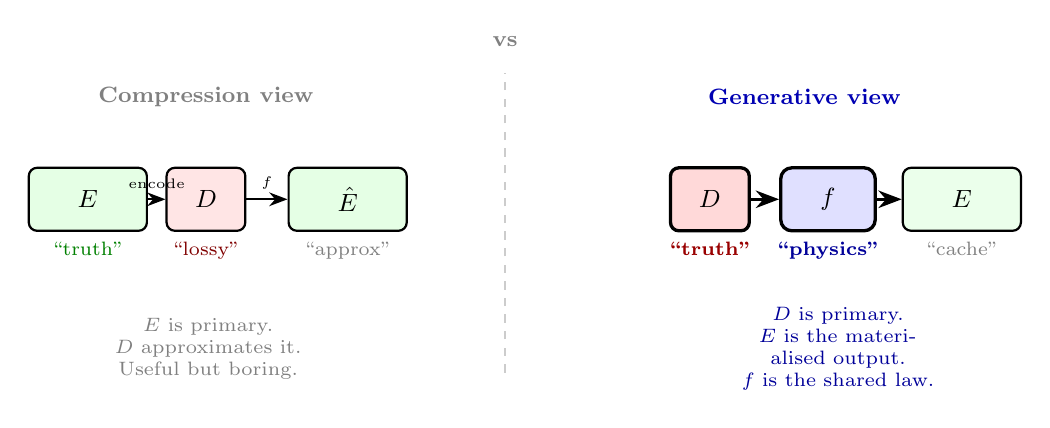
\begin{tikzpicture}[>=Stealth, font=\small]

% ── LEFT: Compression view ────────────────────────────────────────
\begin{scope}[shift={(-3.8, 0)}]
    \node[font=\bfseries\footnotesize, gray] at (0, 2.5) {Compression view};

    % E -> compress -> D -> decompress -> E'
    \node[draw, thick, fill=green!10, rounded corners=3pt,
          minimum width=1.5cm, minimum height=0.8cm] (E1) at (-1.5, 1.2) {$E$};
    \node[font=\scriptsize, green!50!black, below] at (E1.south) {``truth''};

    \node[draw, thick, fill=red!10, rounded corners=3pt,
          minimum width=1.0cm, minimum height=0.8cm] (D1) at (0, 1.2) {$D$};
    \node[font=\scriptsize, red!50!black, below] at (D1.south) {``lossy''};

    \node[draw, thick, fill=green!10, rounded corners=3pt,
          minimum width=1.5cm, minimum height=0.8cm] (E1r) at (1.8, 1.2) {$\hat{E}$};
    \node[font=\scriptsize, gray, below] at (E1r.south) {``approx''};

    \draw[->, thick] (E1) -- (D1) node[midway, above, font=\tiny] {encode};
    \draw[->, thick] (D1) -- (E1r) node[midway, above, font=\tiny] {$f$};

    \node[font=\scriptsize, gray, text width=3cm, align=center] at (0, -0.7)
        {$E$ is primary.\\$D$ approximates it.\\Useful but boring.};
\end{scope}

% ── RIGHT: Generative view ────────────────────────────────────────
\begin{scope}[shift={(3.8, 0)}]
    \node[font=\bfseries\footnotesize, blue!70!black] at (0, 2.5) {Generative view};

    % D -> f -> E (D is primary)
    \node[draw, very thick, fill=red!15, rounded corners=3pt,
          minimum width=1.0cm, minimum height=0.8cm] (D2) at (-1.2, 1.2) {$D$};
    \node[font=\scriptsize, red!60!black, below] at (D2.south) {\textbf{``truth''}};

    \node[draw, very thick, fill=blue!12, rounded corners=4pt,
          minimum width=1.2cm, minimum height=0.8cm] (f2) at (0.3, 1.2) {$f$};
    \node[font=\scriptsize, blue!60!black, below] at (f2.south) {\textbf{``physics''}};

    \node[draw, thick, fill=green!8, rounded corners=3pt,
          minimum width=1.5cm, minimum height=0.8cm] (E2) at (2.0, 1.2) {$E$};
    \node[font=\scriptsize, gray, below] at (E2.south) {``cache''};

    \draw[->, very thick] (D2) -- (f2);
    \draw[->, very thick] (f2) -- (E2);

    \node[font=\scriptsize, blue!60!black, text width=3cm, align=center] at (0.4, -0.7)
        {$D$ is primary.\\$E$ is the materialised output.\\$f$ is the shared law.};
\end{scope}

% Divider
\draw[dashed, gray!40, thick] (0, -1.0) -- (0, 2.8);
\node[font=\bfseries\footnotesize, gray] at (0, 3.2) {vs};

\end{tikzpicture}
\caption{\textbf{Two readings of $f(D) \approx E$.}
\textbf{Left:} $E$ is the ground truth and $D$ is a lossy compression.
\textbf{Right:} $D$ is the native coordinate system; $E$ is a materialised cache of $f(D)$;
$f$ is the shared dynamical law.
The generative view is the one that changes what the model learns:
the lookup table is not compressed---it is \emph{replaced} by a more fundamental representation.}
\label{fig:two-views}
\end{figure}


% ======================================================================
\section{Mathematical Framework}

\subsection{The Phase Space of Token Representations}

Let $\calM$ be the representation manifold---the space of possible token representations.
In a standard transformer, $\calM = \R^d$ and each token is a point.
In the orbital framework, a token is not a point but a \emph{trajectory}---a path through $\calM$ generated by iterating shared dynamics.

\begin{definition}[Phase space]
The phase space $\calM$ is a smooth manifold equipped with a Riemannian metric induced by the shared coupling tensor $\M$.
For $\x, \mathbf{y} \in T_p\calM$ (tangent vectors at point $p$), the inner product is:
\[
    \langle \x, \mathbf{y} \rangle_\M = \x^\top \M\, \mathbf{y}
\]
This metric defines distances, angles, and geodesics in the representation space.
Tokens that are ``similar'' in the coupling geometry are close in this metric.
\end{definition}

In practice, $\calM = \R^d$ and $\M = AB^\top$ is the shared asymmetric coupling matrix.
The metric is not symmetric (asymmetric $\M$), so $\calM$ is more precisely a Finsler manifold than a Riemannian one.
For the present analysis, the asymmetry is important for coupling but the manifold structure is what matters for embeddings.

\subsection{Orbits as Representations}

\begin{definition}[Orbital embedding]
Given a dynamical system $\Phi: \calM \to \calM$ defined by one iteration of the shared ORN block, and a seed point $\s_w \in \calM$ for token $w$, the orbital embedding is the trajectory:
\[
    \calO_w = (\s_w, \Phi(\s_w), \Phi^2(\s_w), \ldots, \Phi^T(\s_w))
\]
The representation of token $w$ at depth $t$ is $\Phi^t(\s_w)$---the point reached after $t$ iterations of the shared dynamics starting from seed $\s_w$.
\end{definition}

This is a group action.
The dynamical system $\Phi$ generates a semigroup $\{\Phi^0, \Phi^1, \Phi^2, \ldots\}$ acting on $\calM$.
The orbit of seed $\s_w$ under this action \emph{is} the token's representation across depths.

\begin{definition}[Orbit equivalence]
Two tokens $w_1, w_2$ are \emph{orbitally equivalent} if their orbits converge:
\[
    w_1 \sim w_2 \iff \lim_{t \to \infty} \| \Phi^t(\s_{w_1}) - \Phi^t(\s_{w_2}) \| = 0
\]
Orbitally equivalent tokens are functionally interchangeable---they reach the same attractor regardless of their surface form.
\end{definition}

In a children's story dataset, ``Emma'', ``Max'', ``Lily'' should be orbitally equivalent: they are all instances of the CHILD-CHARACTER role.
Their seeds differ (the model can distinguish them) but their orbits converge (the model treats them identically for structural purposes).

\subsection{The Standard Transformer as a Trivial Orbit}

In a standard transformer, the ``orbit'' is degenerate:
\[
    \calO_w^{\text{transformer}} = (\mathbf{e}_w, f_1(\mathbf{e}_w, \text{context}), f_2(f_1(\ldots), \text{context}), \ldots)
\]
where each $f_l$ uses different parameters ($W_Q^{(l)}, W_K^{(l)}$, etc.).
The seed $\mathbf{e}_w$ is a full $d$-dimensional vector---it already contains the complete representation.
The ``dynamics'' at each layer use different rules.
There is no generator; each layer is a separate lookup of what transformation to apply.

\begin{figure}[h]
\centering
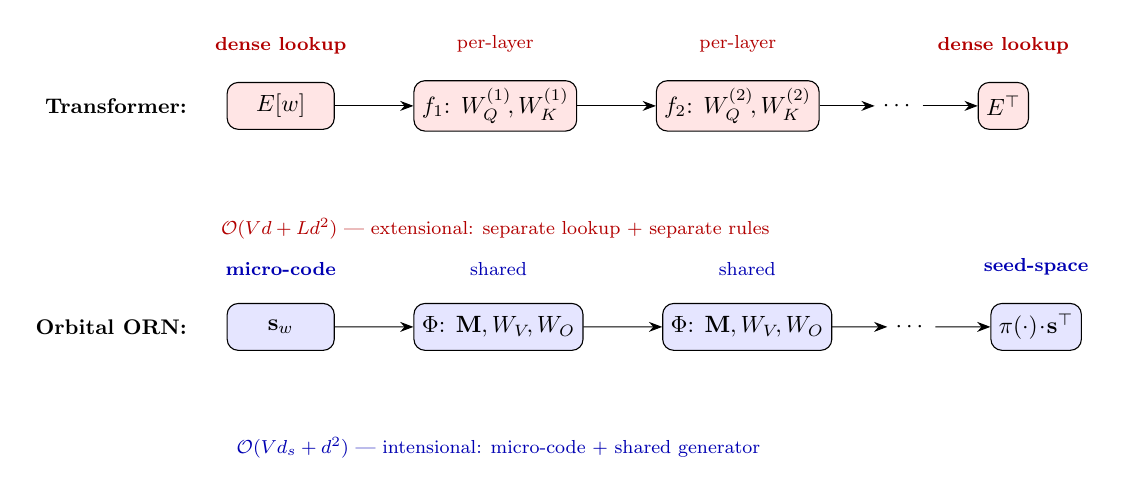
\begin{tikzpicture}[>=Stealth, node distance=1.8cm, scale=0.85, every node/.style={scale=0.85}]
    % Transformer
    \node[draw, rounded corners, fill=red!10, minimum width=1.6cm, minimum height=0.7cm] (emb) {$E[w]$};
    \node[draw, rounded corners, fill=red!10, right=1.0cm of emb, minimum height=0.7cm] (l1) {$f_1$: $W_Q^{(1)}\!,W_K^{(1)}$};
    \node[draw, rounded corners, fill=red!10, right=1.0cm of l1, minimum height=0.7cm] (l2) {$f_2$: $W_Q^{(2)}\!,W_K^{(2)}$};
    \node[right=0.7cm of l2] (dots1) {$\cdots$};
    \node[draw, rounded corners, fill=red!10, right=0.7cm of dots1, minimum height=0.7cm] (out) {$E^\top$};

    \draw[->] (emb) -- (l1);
    \draw[->] (l1) -- (l2);
    \draw[->] (l2) -- (dots1);
    \draw[->] (dots1) -- (out);

    \node[above=0.25cm of emb, text=red!70!black, font=\footnotesize\bfseries] {dense lookup};
    \node[above=0.25cm of l1, text=red!70!black, font=\footnotesize] {per-layer};
    \node[above=0.25cm of l2, text=red!70!black, font=\footnotesize] {per-layer};
    \node[above=0.25cm of out, text=red!70!black, font=\footnotesize\bfseries] {dense lookup};

    \node[left=0.4cm of emb, font=\small\bfseries] {Transformer:};

    % ORN Orbit
    \node[draw, rounded corners, fill=blue!10, minimum width=1.6cm, minimum height=0.7cm, below=2.2cm of emb] (seed) {$\s_w$};
    \node[draw, rounded corners, fill=blue!10, right=1.0cm of seed, minimum height=0.7cm] (p1) {$\Phi$: $\M,W_V\!,W_O$};
    \node[draw, rounded corners, fill=blue!10, right=1.0cm of p1, minimum height=0.7cm] (p2) {$\Phi$: $\M,W_V\!,W_O$};
    \node[right=0.7cm of p2] (dots2) {$\cdots$};
    \node[draw, rounded corners, fill=blue!10, right=0.7cm of dots2, minimum height=0.7cm] (out2) {$\pi(\cdot) \!\cdot\! \s^\top$};

    \draw[->] (seed) -- (p1);
    \draw[->] (p1) -- (p2);
    \draw[->] (p2) -- (dots2);
    \draw[->] (dots2) -- (out2);

    \node[above=0.25cm of seed, text=blue!70!black, font=\footnotesize\bfseries] {micro-code};
    \node[above=0.25cm of p1, text=blue!70!black, font=\footnotesize] {shared};
    \node[above=0.25cm of p2, text=blue!70!black, font=\footnotesize] {shared};
    \node[above=0.25cm of out2, text=blue!70!black, font=\footnotesize\bfseries] {seed-space};

    \node[left=0.4cm of seed, font=\small\bfseries] {Orbital ORN:};

    % Annotations
    \node[below=1.0cm of l1, text=red!70!black, font=\footnotesize, align=center] {$\bigO(Vd + Ld^2)$ --- extensional: separate lookup $+$ separate rules};
    \node[below=1.0cm of p1, text=blue!70!black, font=\footnotesize, align=center] {$\bigO(Vd_s + d^2)$ --- intensional: micro-code $+$ shared generator};

\end{tikzpicture}
\caption{Architectural comparison.
\textbf{Top:} Standard transformer.
Token enters via dense lookup ($V \times d$), each layer applies different weights, output via dense lookup.
\textbf{Bottom:} Orbital ORN.
Token enters as micro-code ($V \times d_{\text{seed}}$), the same shared block $\Phi$ iterates to generate the representation, output projects back to seed space.
The entire model is one dynamical system.}
\label{fig:arch-comparison}
\end{figure}


\subsection{Group-Theoretic View}

\paragraph{Connection to semigroup theory.}
The dynamical system $\Phi$ generates a \emph{semigroup} of operators $\{\Phi^0, \Phi^1, \Phi^2, \ldots\}$ (a semigroup rather than a group because $\Phi$ need not be invertible).
Chen \& Wu~\cite{chen2023deeposg} showed that explicitly embedding the semigroup property $T(s+t) = T(s) \circ T(t)$ into neural architectures \emph{dramatically reduces data dependency} and improves long-time prediction.
This parallels our finding: memoisation (shared $\M$) works with no quality loss because we are implicitly enforcing algebraic consistency on the coupling dynamics.

Vacher~\cite{vacher2026ifs} formalises deep networks as \emph{iterated function systems} (IFS), proving existence of invariant measures under contractivity and deriving Wasserstein generalisation bounds.
The orbital embedding is an IFS: the shared block $\Phi$ is the iterated map, the seeds $\s_w$ are initial conditions, and the attractors correspond to semantic roles.

Let $G$ be the group generated by $\Phi$.
In the orbital model, the representation of token $w$ is the orbit $G \cdot \s_w$---the set of all points reachable from seed $\s_w$ by applying elements of $G$.

\begin{proposition}[Orbit--stabiliser structure]
For each seed $\s_w$, the orbit $G \cdot \s_w$ and the stabiliser $G_{\s_w} = \{g \in G : g \cdot \s_w = \s_w\}$ satisfy:
\[
    |G| = |G \cdot \s_w| \times |G_{\s_w}|
\]
Tokens with large stabilisers (many iterations leave them unchanged) are at or near fixed points---they have stable, attractor-like representations.
Tokens with small stabilisers (each iteration changes them significantly) are in transient regions---their representations are still forming.
\end{proposition}

The group $G$ is the same for all tokens---it is determined by $\M$ and the shared block.
Different tokens explore different parts of the same group's action.
This is exactly the ``generators, not trajectories'' idea: $G$ is compact (one shared block), but $G \cdot \s_w$ can be arbitrarily complex.

\subsection{The Geometry of Convergence}

Define the \emph{orbital distance} between tokens as:
\[
    d_{\text{orbit}}(w_1, w_2) = \sum_{t=0}^{T} \alpha_t \| \Phi^t(\s_{w_1}) - \Phi^t(\s_{w_2}) \|_\M
\]
where $\alpha_t$ are weights (e.g., exponentially increasing to emphasise later iterations where the representation has stabilised).

This metric captures something the Euclidean distance between embedding vectors cannot: \emph{functional similarity is measured by convergent dynamics, not by proximity in a lookup table}.

Two tokens may start far apart (different seeds) but converge under iteration---they are functionally equivalent.
Two tokens may start nearby (similar surface forms) but diverge under iteration---they have different roles.

\begin{remark}[Basins of attraction]
If $\Phi$ has attractors $\{A_1, A_2, \ldots, A_k\}$, then the vocabulary is partitioned into basins:
$B_i = \{w : \Phi^T(\s_w) \approx A_i\}$.
Each basin corresponds to a functional role.
The number of attractors $k$ is the effective number of roles the geometry has learned.
This is directly measurable: count the number of distinct clusters in $\{\Phi^T(\s_w)\}_{w \in V}$.
\end{remark}


% ======================================================================
\section{The Bootstrap Problem}

\subsection{Why This Is Hard}

In a standard transformer, the embedding table provides a ``warm start''---every token begins with a rich, distinct $d$-dimensional vector.
The attention mechanism receives well-separated inputs from step zero.

In the orbital model, every token starts as a point in a $d_{\text{seed}}$-dimensional space, projected into $\R^d$.
At iteration $t{=}0$, the representations are low-rank---they live in a $d_{\text{seed}}$-dimensional subspace of $\R^d$.
The attention mechanism must bootstrap from these impoverished inputs.

\paragraph{The chicken-and-egg problem.}
The shared block $\Phi$ (including $\M$) must learn to:
\begin{enumerate}[nosep]
    \item \emph{Generate} meaningful representations from seeds (the embedding function).
    \item \emph{Process} context by routing information between tokens (the attention function).
    \item \emph{Transform} representations via the FFN (the knowledge function).
\end{enumerate}
These are three different jobs performed by the same shared weights.
At initialisation, none of them work---the representations are random, the coupling is random, and the transforms are random.
There is no gradient signal to shape any of them because the others are broken.

This is the fundamental training challenge.
It does not arise in the standard transformer because the embedding table provides (1) independently of (2) and (3), and per-layer weights separate (2) and (3) across depth.

\subsection{Candidate Solutions}

\paragraph{Curriculum: seed $\to$ orbit in stages.}
\begin{enumerate}[nosep]
    \item \textbf{Phase 1:} Train with a standard embedding table (dense lookup). Learn $\M$ and the shared block.
    \item \textbf{Phase 2:} Compress the learned embeddings into seeds via projection. Fine-tune with orbital dynamics, gradually reducing $d_{\text{seed}}$.
    \item \textbf{Phase 3:} Remove the dense table entirely. Seeds only.
\end{enumerate}
This is distillation: the dense model teaches the orbital model what the geometry should look like.
The risk is that the orbital model inherits the trajectory structure of the dense model rather than learning its own generators.

\paragraph{Auxiliary reconstruction loss.}
During training, add a loss term that forces the orbital representation to reconstruct a target embedding:
\[
    \calL_{\text{recon}} = \| \Phi^T(\s_w) - \mathbf{e}_w^{\text{target}} \|^2
\]
where $\mathbf{e}_w^{\text{target}}$ comes from a pretrained embedding table or is co-trained.
This provides gradient signal for the orbit even when the language modelling loss is uninformative.
The reconstruction weight is annealed to zero as training progresses.

\paragraph{Increasing iteration depth.}
Start with $T = 1$ (essentially a learned projection from seed space) and gradually increase $T$ during training.
At $T = 1$, the model is a standard neural network with a bottleneck embedding.
At $T > 1$, the orbital dynamics begin to contribute.
This avoids the cold-start problem: the model learns a useful projection first, then learns to iterate.

\paragraph{Ontological scaffolding (see Section~5).}
Use a parallel system that provides dense, token-specific information as a ``hint'' during the early iterations.
As the orbital geometry matures, the scaffolding is removed or reduced to handling only genuinely discrete information.


% ======================================================================
\section{The Two-System Architecture}\label{sec:twosystem}

\subsection{The Core Tension}

Natural language mixes two kinds of information:

\begin{description}[nosep, leftmargin=1.5em]
    \item[Structural:] ``A character wanted something, faced an obstacle, resolved it.'' \\
    This is orbital---it is a path through narrative space, invariant across specific instances.

    \item[Referential:] ``Caesar crossed the Rubicon in 49~BC.'' \\
    This is discrete---it binds a specific name to a specific event. No amount of geometric iteration derives ``49~BC'' from the structure of ``ruler crosses a boundary.''
\end{description}

The orbital model handles structural knowledge naturally.
Referential knowledge is the problem.
A dense embedding table handles both, badly: it wastes capacity on redundant structural representations in order to store the occasional specific fact.

\subsection{The Parallel Ontological Layer}

We conjecture that the correct architecture has two parallel systems:

\begin{figure}[h]
\centering
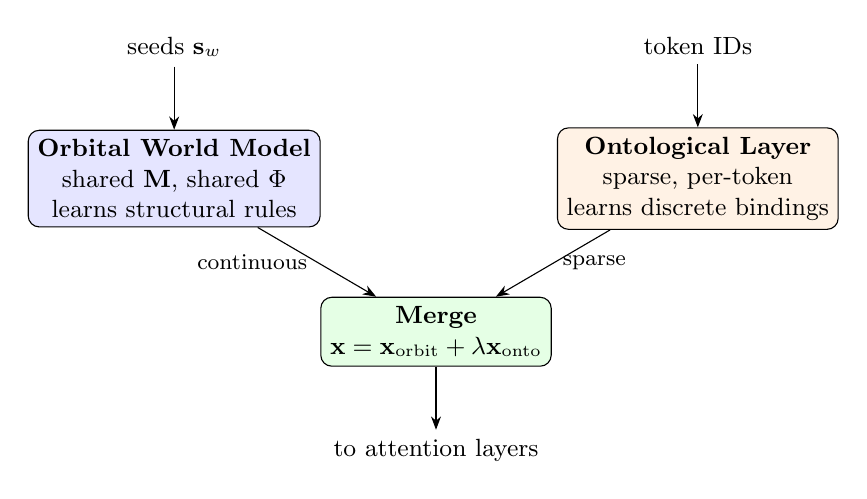
\begin{tikzpicture}[>=Stealth, node distance=1.8cm, font=\small]
    \node[draw, rounded corners, fill=blue!10, minimum width=3cm, minimum height=1cm, align=center] (orbit) {\textbf{Orbital World Model}\\shared $\M$, shared $\Phi$\\learns structural rules};

    \node[draw, rounded corners, fill=orange!10, minimum width=3cm, minimum height=1cm, align=center, right=3cm of orbit] (onto) {\textbf{Ontological Layer}\\sparse, per-token\\learns discrete bindings};

    \node[draw, rounded corners, fill=green!10, minimum width=2.5cm, minimum height=0.8cm, below=1.5cm of $(orbit)!0.5!(onto)$, align=center] (merge) {\textbf{Merge}\\$\x = \x_{\text{orbit}} + \lambda \x_{\text{onto}}$};

    \node[above=0.8cm of orbit, align=center] (seeds) {seeds $\s_w$};
    \node[above=0.8cm of onto, align=center] (tokens) {token IDs};

    \draw[->] (seeds) -- (orbit);
    \draw[->] (tokens) -- (onto);
    \draw[->] (orbit) -- (merge) node[midway, left, font=\footnotesize] {continuous};
    \draw[->] (onto) -- (merge) node[midway, right, font=\footnotesize] {sparse};

    \node[below=0.8cm of merge] (out) {to attention layers};
    \draw[->] (merge) -- (out);
\end{tikzpicture}
\caption{Two-system architecture.
The orbital world model generates structural representations from seeds via shared dynamics.
The ontological layer provides sparse, token-specific bindings for referential information.
The merge is additive with a learned or annealed gate $\lambda$.
During training, $\lambda$ starts high (the ontological layer scaffolds learning) and decreases as the orbital geometry matures.
At convergence, the ontological layer handles only genuinely discrete information.}
\label{fig:two-system}
\end{figure}

\paragraph{The orbital world model} (our ORN) learns structural rules.
It knows ``when a character wants something, an obstacle follows.''
It does not know that Emma is a girl or that Caesar ruled Rome.
Its representations are continuous orbits in $\M$'s geometry.
All heads share the same coupling rules.

\paragraph{The ontological layer} learns discrete bindings.
It is a sparse, per-token system---closer to a key--value store than a neural network.
It maps token IDs to low-rank perturbations: $\x_{\text{onto}} = U_w$ where $U_w \in \R^d$ is a sparse or low-rank vector specific to token $w$.
This is where ``Caesar $\to$ Roman, ruler, betrayed'' lives.

\paragraph{The merge.}
The final representation is:
\[
    \x_w = \Phi^T(\s_w) + \lambda \cdot U_w
\]
where $\lambda$ is a gate that controls how much ontological information to inject.

\paragraph{The critical constraint: force structure into the orbit.}
If $\lambda$ is unconstrained, the model will collapse to $\lambda = 1$ and use the ontological layer for everything---recreating a dense embedding table.
The architectural enforcement is:
\begin{itemize}[nosep]
    \item $U_w$ is low-rank (rank $r \ll d$) or sparse (at most $k$ nonzero entries).
    \item $\lambda$ is regularised or annealed: $\lambda(t) = \lambda_0 \cdot e^{-\beta t}$.
    \item The ontological layer has a strict parameter budget: $V \times r$ for rank-$r$, much less than $V \times d$.
    \item All attention heads use M from the orbital model, never the ontological perturbations, for coupling. The ontological layer adds to the value stream only.
\end{itemize}

This forces the model to use the orbital system for everything it can, and the ontological layer only for what it must.

\subsection{Biological Analogy}

This maps cleanly to the cortex--hippocampus division~\cite{mcclelland1995complementary}:

\begin{center}\small
\begin{tabular}{@{}lll@{}}
\toprule
& \textbf{Cortex} (orbital) & \textbf{Hippocampus} (ontological) \\
\midrule
Stores & Generators, attractors, rules & Specific episodes, bindings \\
Updates & Slowly (gradient descent) & Rapidly (one-shot binding) \\
Representation & Continuous, distributed & Sparse, localist \\
Failure mode & Can't remember names & Can't generalise \\
\bottomrule
\end{tabular}
\end{center}

The transformer collapses both into a single system (dense weight matrices) and asks gradient descent to sort out the mix.
This works---transformers are powerful---but it is inefficient: you need enormous capacity because the storage format is wrong for both jobs.

\subsection{Design Progression: Where Does the Ontological Layer Sit?}

The two-system architecture has a critical design question: how does the ontological layer interact with the attention block?
We identify three designs in a natural progression from our pure orbital network:

\paragraph{Design A: Static per-token correction (value-stream only).}
A small per-token embedding $u_w \in \R^r$ ($r \ll d$) is projected to $d_{\text{model}}$ and added to the value input at every layer.
The coupling ($Q, K$ from shared $\M$) sees only the orbital stream; the ontological signal enters through values only.
\textit{Problem:} ``Lily'' gets the same correction vector in every context.
Cannot do contextual binding.
Exp~4b tests this design; early results show minimal contribution ($-1.7\%$ onto gap).

\paragraph{Design B: Ontological values riding $\M$'s coupling.}
The ontological layer has its own value projection $W_V^{\text{onto}}$ but uses $\M$ for coupling.
The attention pattern (who talks to whom) is structural; the content that flows through it is identity-enriched.
\textit{Problem:} cannot do identity-dependent routing.
Coreference (``She'' $\to$ ``Lily'' not ``cake'') requires identity information in the coupling, not just the values.
Exp~4c tests this design with annealed $\lambda$.

\paragraph{Design C: Dual-pathway attention (parallel orbital + ontological).}
The attention block contains \textbf{two parallel pathways}:

\begin{enumerate}[nosep]
    \item \textbf{Orbital pathway} (cortex-like): uses shared $\M$ for coupling, per-layer $W_V, W_O$ for response.
    Large capacity ($d^2$ coupling, $d^2$ response). Handles structural rules.

    \item \textbf{Ontological pathway} (hippocampus-like): has its \emph{own} tiny $W_Q^{\text{onto}}, W_K^{\text{onto}}, W_V^{\text{onto}}$, all operating in $r$ dimensions.
    Capacity-constrained ($r^2$ coupling, $r \times d$ projections). Handles identity routing.
\end{enumerate}

\noindent
Both pathways operate on the same input and combine at the output:
\[
    \x_{l+1} = \x_l + \underbrace{W_O \left(\text{attn}_{\M}(\x_l) \cdot W_V(\x_l)\right)}_{\text{orbital: structural response}} + \underbrace{W_O^{\text{onto}} \left(\text{attn}_{\text{onto}}(\x_l, u) \cdot W_V^{\text{onto}}(u)\right)}_{\text{ontological: identity routing}}
\]

The orbital pathway cannot see the ontological codes---$\M$ remains pure structural.
The ontological pathway has its own attention mechanism and can route by identity (coreference, entity tracking).
But it operates in $r$ dimensions ($r = 4$--$8$), so it physically cannot replace $\M$: it can carry a few bits of identity information, not the full coupling geometry.

\paragraph{The constraint is architectural, not just regularisation.}
In our implementation, the ontological pathway uses $2.8\%$ of total parameters (215K out of 7.7M).
Even if gradient descent tried to route everything through onto, the rank-$r$ bottleneck prevents it.
$\M$ wins by sheer capacity; onto fills the gaps.

\paragraph{Training dynamics: who trains first?}
In the dual-pathway design with $\lambda = 1$ from step~0, we predict the ontological pathway trains first (path of least resistance): it provides per-token identity signal immediately via its own $Q, K$, while $\M$ is still random.
As training progresses, $\M$ develops structural coupling and dominates by capacity.
The ontological contribution should peak early and decline proportionally---not because it is annealed, but because $\M$ takes over.

This gives the ontological layer two distinct roles:
\begin{description}[nosep]
    \item[During training: bootstrapper.] Provides early gradient signal while $\M$ develops.
    The system can learn before the orbital geometry is ready.
    \item[After training: fine-tuning surface.] Freeze $\M$ and the orbital response heads.
    Swap or fine-tune only the ontological codes and projections for a new domain.
    Cheap, targeted adaptation without touching the world model.
\end{description}

\noindent
Exp~4d tests this design. The critical diagnostic: the \texttt{onto\_gap} (loss with vs.\ without ontological pathway) measured over training.
If it peaks early and declines, the bootstrapping hypothesis is confirmed.

\paragraph{Exp~7 result: Design C underperforms at 10M.}
At matched 10M parameters on TinyStories (5000 steps), Design~C (SharedM+Onto with $r{=}4$ parallel attention) scored 2.929 vs.\ SharedM-alone at 2.855 and the transformer at 2.830.
The ontological pathway contributed only ${\sim}1.5\%$ improvement over ablation (setting $\lambda{=}0$) while consuming parameter budget that would otherwise increase depth or width.
The parallel attention mechanism competes with $\M$ rather than complementing it.

\paragraph{Design D: Perturbative corrections (the path integral analogy).}
The exp7 failure motivates a redesign.
The orbital model produces the \emph{classical path}---the dominant trajectory through $\M$'s coupling geometry.
Context provides the boundary conditions.
The ontological correction should be a \emph{perturbation} around this path, not a parallel system:
\[
    \x^{(\ell)} = \x^{(\ell)}_{\text{orbital}} + g(\x^{(\ell)}) \cdot \delta(\x^{(\ell)})
\]
where $g: \R^d \to \R^+$ is a context gate (sigmoid of a learned linear projection of the residual stream) and $\delta$ is a small correction MLP ($d \to d_{\text{corr}} \to d$, with $d_{\text{corr}} \ll d$).

Key properties:
\begin{itemize}[nosep]
    \item No separate attention. The perturbation reads from the residual stream (which already encodes context via $\M$'s coupling) and produces a residual correction.
    \item $g \approx 0$ without context: early tokens or isolated tokens get pure orbital output. As context accumulates, the gate opens and the correction tightens the prediction.
    \item The gate bias is initialised negative (${\sim}{-}3$, so $\sigma \approx 0.05$) and the correction output is initialised at zero. The perturbation starts near zero and must be learned.
    \item $\|\delta\| \ll \|\x_{\text{orbital}}\|$: it is a correction, not a replacement. If the perturbation overwhelms the orbital signal, the architecture has degenerated.
\end{itemize}

\noindent
This is analogous to path integrals in physics: the semigroup gives the classical trajectory, and the perturbation provides context-dependent quantum corrections around it.

An important distinction (explored in detail in the companion document \textit{Path Integrals and the ORN}): the ORN is \emph{not} a path integral and should not be.
The path integral computes $T^L$ (the propagator---averaging over all possible intermediate paths), which converges to the stationary distribution at large $L$, forgetting the starting context.
The ORN uses the same semigroup structure as a geometric scaffold, but its deeper layers \emph{refine} the context-specific prediction rather than \emph{composing} statistical propagators.
The coupling geometry is the grammar; the response heads speak the language.
This is why the ORN preserves context (via the residual connection) while a path integral would average it away.

More precisely: the ORN computes a path integral along an orbit in representation space, where the ``action'' is determined by the shared coupling geometry $\M$, the ``renormalisation'' is performed by per-layer response heads, and the ``quantum corrections'' are supplied by the perturbative gate.
The distinction from a standard path integral is that the ORN's integral \emph{selects} among possibilities (contextual refinement) rather than \emph{averaging} over them (statistical propagation).

The diagnostic predictions: (i)~$\bar{g}$ increases over training as context representations mature; (ii)~$\|\delta\|/\|\x\|$ remains small; (iii)~ablating the perturbation hurts late-sequence tokens (rich context) more than early tokens (little context).

\paragraph{Exp~8 results (10M, external machine).}
All three predictions are confirmed.
The perturbative model (d=172, L=4, 10.03M params) was forced to sacrifice a full layer vs SharedM (d=168, L=5, 9.96M params) for param matching---and still recovered to match SharedM by step~2{,}500:

\begin{center}\small
\begin{tabular}{@{}rcccccc@{}}
\toprule
Step & SharedM & Perturbative & $\Delta$ & Gate $\bar{g}$ & $\|\delta\|/\|h\|$ & Attn $H$ \\
\midrule
500 & 4.276 & 4.258 & $-0.018$ & 0.247 & 0.800 & 4.43 \\
2500 & 2.975 & 2.974 & $-0.001$ & 0.348 & 0.571 & 3.30 \\
4000 & 2.797 & 2.787 & $-0.010$ & 0.360 & 0.567 & 3.23 \\
\bottomrule
\end{tabular}
\end{center}

\noindent The gate opened from 0.05 to 0.36 (prediction~i confirmed).
The perturbation ratio settled at ${\sim}0.57$; the effective contribution is $g \times \delta/h \approx 0.20$ (prediction~ii confirmed---genuinely perturbative).
The gate anticorrelates with attention entropy: corrections activate when coupling is confident, not when it is diffuse.
Prediction~iii (late-position benefit) awaits the ablation from the completed run.

The crossover dynamics are the same as SharedM vs transformer: structural investment early (corrections dormant, the missing layer hurts), exploitation late (gate opens, corrections compensate).
Recovering a full layer of orbital depth through 1.1\% parameter overhead of structured corrections is a strong signal that the perturbative design is architecturally sound.

An ablation study provides the strongest evidence: disabling the corrections at inference (forcing $g{=}0$) increases val loss from 2.755 to 3.204---a gap of \textbf{0.449~nats}.
This is larger than the entire improvement from step~1{,}000 to step~5{,}000 for SharedM alone.
Per-position analysis confirms prediction~(iii): late positions benefit more (+0.440 nats) than early (+0.392), though both are large.

The ablation also reveals that the orbital backbone \emph{co-adapted} with the corrections: it offloaded ${\sim}0.45$ nats of work to the correction pathway and reorganised its own coupling accordingly.
The perturbative model learned a different orbital solution than standalone SharedM---the two systems are coupled, not independent.

The matched-depth follow-up (Exp~8b: same d, L as SharedM, corrections as extra params) is the clean test.
If perturbative at matched depth beats SharedM, the corrections add genuine value beyond compensating for lost depth.
This result determines whether the full ORN architecture (SharedM + perturbative corrections) scales to 50M.


% ======================================================================
\section{The Training Problem: Micro-Experiments}

The full orbital architecture is hard to train because everything depends on everything else.
We decompose the problem into independently testable components.

\subsection{Level 0: Can Orbital Dynamics Generate Useful Embeddings?}

\paragraph{Setup.}
Take a pretrained embedding table $E \in \R^{V \times d}$.
Learn seeds $\s_w \in \R^{d_{\text{seed}}}$ and a shared block $\Phi$ such that $\Phi^T(\text{proj}(\s_w)) \approx \mathbf{e}_w$ for all $w$.
This is pure reconstruction---no language modelling.

\paragraph{Measurements.}
\begin{itemize}[nosep]
    \item Reconstruction error vs.\ $d_{\text{seed}}$ and $T$ (how much seed and how many iterations are needed?)
    \item Does $\Phi$ learn meaningful dynamics? (Check eigenspectrum, attractor structure.)
    \item Do orbitally equivalent tokens (Emma/Max/Lily) get similar seeds?
    \item What is the effective rank of the seed space? (How many functional roles emerge?)
\end{itemize}

\paragraph{Kill criterion.}
If reconstruction requires $d_{\text{seed}} > d/2$, the orbit adds no compression and the framework fails.

\subsection{Level 1: Orbital Embeddings in a Fixed Model}

\paragraph{Setup.}
Take a pretrained ORN (shared $\M$, per-layer V/O as in current experiments).
Replace the dense embedding table with seeds + a small orbital pre-processor that uses $\M$.
Freeze the main model.
Train only the seeds and the seed projection.

\paragraph{Question.}
Can orbital embeddings feed a working language model?
This isolates the embedding question from the training dynamics question.

\paragraph{Kill criterion.}
Validation loss more than $50\%$ worse than the dense embedding version.

\subsection{Level 2: Joint Training with Orbital Embeddings}

\paragraph{Setup.}
Train the full orbital ORN from scratch: seeds, shared block, no dense table.
Use the curriculum strategy: start with $T_{\text{embed}} = 1$ (linear projection), gradually increase to full iteration.

\paragraph{Question.}
Can the orbital embedding and the processing dynamics co-learn from scratch?

\paragraph{Measurements.}
\begin{itemize}[nosep]
    \item Loss curve compared to dense-embedding ORN at matched total params.
    \item Orbit convergence: does $\|\Phi^t(\s_w) - \Phi^{t-1}(\s_w)\|$ decrease?
    \item Attractor count: how many clusters form in $\{\Phi^T(\s_w)\}$?
    \item Scaling exponent: is $\beta$ different from the dense-embedding model?
\end{itemize}

\paragraph{Kill criterion.}
Loss more than $30\%$ worse at all scales, OR orbits do not converge (representations remain chaotic).

\subsection{Level 3: Ontological Scaffolding}

\paragraph{Setup.}
Add the ontological layer: sparse per-token perturbations $U_w$ (rank $r$).
Train jointly with the orbital model.
Anneal $\lambda$ from 1.0 to 0.1 over training.

\paragraph{Question.}
Does the ontological layer handle the ``Caesar problem'' (specific referential knowledge) while the orbital model handles structure?

\paragraph{Measurements.}
\begin{itemize}[nosep]
    \item Which tokens have large $\|U_w\|$? (Should be proper nouns, specific entities, rare tokens.)
    \item Which tokens have small $\|U_w\|$? (Should be function words, common verbs, structural tokens.)
    \item If we ablate the ontological layer at test time, which capabilities degrade?
\end{itemize}

\paragraph{Kill criterion.}
The model collapses to using ontological layer for everything ($\|U_w\|$ large for all tokens, orbital representations unused).

\subsection{Level 4: Full Orbital + Ontological at Scale}

\paragraph{Setup.}
Train both systems jointly on TinyStories at $\{2\text{M}, 5\text{M}, 10\text{M}\}$ parameters.
Compare against: (a) standard transformer, (b) coupling-only ORN (our current architecture), (c) orbital ORN without ontological layer.

\paragraph{The key prediction.}
The orbital + ontological model should have a steeper scaling exponent than all baselines.
The ontological layer's parameter footprint should grow sub-linearly with $V$ (only genuinely discrete tokens need large perturbations).
The orbital model's parameter footprint should be nearly independent of $V$.


% ======================================================================
\section{The Representation-Theoretic Picture}

\subsection{Tokens as Group Representations}

A group $G$ (generated by $\Phi$) acts on the phase space $\calM$.
Each token $w$ defines an orbit $G \cdot \s_w$.
The map $w \mapsto G \cdot \s_w$ is a \emph{representation} of the vocabulary in the space of $G$-orbits.

In representation theory, a representation is \emph{irreducible} if it cannot be decomposed into smaller invariant subspaces.
The orbital embedding learns a representation that is as irreducible as possible---the shared geometry forces tokens into a single coherent space rather than allowing independent subspaces for each token.

\subsection{The Tangent Space and Local Linearisation}

At any point $\x_t = \Phi^t(\s_w)$ on the orbit, the tangent space $T_{\x_t}\calM$ describes the local geometry.
The Jacobian of $\Phi$ at $\x_t$:
\[
    J_t = \frac{\partial \Phi}{\partial \x}\bigg|_{\x = \x_t}
\]
describes how small perturbations evolve.
The eigenvalues of $J_t$ determine local stability:
\begin{itemize}[nosep]
    \item $|\lambda_i| < 1$: perturbations along eigenvector $\mathbf{v}_i$ contract. The orbit is locally stable in this direction.
    \item $|\lambda_i| > 1$: perturbations grow. The orbit is locally unstable---small seed differences amplify.
    \item $|\lambda_i| \approx 1$: perturbations neither grow nor shrink. The orbit is locally neutral.
\end{itemize}

For the orbital embedding to work, we need:
\begin{itemize}[nosep]
    \item \textbf{Contracting directions} for structural features (Emma $\approx$ Max $\approx$ Lily should converge).
    \item \textbf{Neutral/expanding directions} for distinguishing features (Emma $\neq$ Max in surface form).
\end{itemize}

This is a \emph{mixed-stability} regime: the dynamics must simultaneously contract some dimensions and preserve others.
This is precisely what attractor dynamics in dissipative systems do---they collapse trajectories onto low-dimensional manifolds while preserving information along the manifold.

\subsection{Connections to Existing Mathematics}

\paragraph{Smooth dynamical systems.}
The orbital embedding is a discrete-time dynamical system on $\R^d$.
The fixed points, limit cycles, and strange attractors of $\Phi$ correspond to stable token representations, oscillating representations, and chaotic representations respectively.
A well-trained model should have clean fixed-point or limit-cycle attractors, not chaos.

\textit{Evidence:} Deep Equilibrium Models~\cite{bai2019deep} demonstrate that fixed-point iteration with a single weight-tied layer achieves competitive performance on WikiText-103 with 88\% memory reduction.
Universal Transformers~\cite{dehghani2018universal} apply the same block repeatedly with a learned halting mechanism, making the architecture Turing-complete (unlike fixed-depth transformers).
Neural ODEs~\cite{chen2018neural} generalise this to continuous depth, training with $\calO(1)$ memory via the adjoint method.
Recent Neural ODE Transformers~\cite{neuralode2025transformer} parameterise transformer weights as continuous functions of depth, treating the layer index as a time variable.
All four support our proposal: \emph{weight sharing across depth works when the underlying dynamics are approximately invariant}.

\paragraph{Riemannian geometry.}
The metric $\M$ induces a geometry on $\calM$.
Geodesics in this geometry are the ``shortest paths'' between token representations.
The orbital dynamics need not follow geodesics---they follow the flow of $\Phi$---but the distance function defined by $\M$ determines the coupling (attention) between tokens.
There is a deep connection: the coupling geometry ($\M$) and the dynamical geometry ($\Phi$) must be compatible.

\textit{Evidence:} Hauser \& Ray~\cite{hauser2017riemannian} established that residual networks perform geometric transformations on data manifolds, with learned weights defining the local metric.
Benfenati \& Marta~\cite{benfenati2022singular} extended this to \emph{singular} Riemannian geometry, handling the degenerate metrics that arise at saddle points and representation collapse regions---precisely the regimes our orbital dynamics must navigate.
A key result~\cite{training2023geometry}: at infinite width with random initialisation, the induced metric is highly symmetric (isotropic).
Feature learning \emph{breaks this symmetry}, creating an anisotropic metric that magnifies differences along decision boundaries.
Our $\M$ develops condition number $> 10$ via SGD---this is the geometric signature of learned structure, not an artefact.

\paragraph{Information geometry.}
If the orbital model is viewed as a statistical model---mapping seeds to probability distributions over next tokens---then the space of models is a statistical manifold with the Fisher information metric.
The shared $\M$ can be interpreted as an approximation to the Fisher metric on this manifold.
This connects the coupling geometry to the information-theoretic structure of the language.
Amari's foundational work~\cite{amari2019fisher} shows that the parameter space of neural networks is a Riemannian manifold with Fisher information metric, and that natural gradient (which descends steepest in this geometry) avoids plateaus that trap ordinary SGD.

\paragraph{Kolmogorov complexity and compression.}
The memoisation hypothesis has a clean information-theoretic interpretation: we claim the coupling rule across $L$ transformer layers has low Kolmogorov complexity $K$---it can be described by a short program (shared $\M$) rather than stored explicitly ($2L$ separate matrices).

\textit{Evidence for:}
Shaw et al.~\cite{shaw2026kolmogorov} formally bridge Kolmogorov complexity and transformers, constructing \emph{asymptotically optimal description length objectives} by mapping transformer weights to prefix Turing machines.
Their result proves transformers can achieve compression quality comparable to $K(x)$ up to an additive constant---validating that our search for compressed representations is theoretically grounded.
Lotfi et al.~\cite{lotfi2024compression} show that models which compress training data more achieve better generalisation, obtaining non-vacuous generalisation bounds for actual LLMs.
The complexity dynamics of grokking~\cite{demoss2024grokking} reveal that networks first memorise (high description length) then compress (low description length)---training actively reduces complexity by finding structure.
Our spectral invariance finding (cosine sim 0.19 but spectrum correlation 0.98 across layers) is exactly the signature of low algorithmic complexity: the \emph{structure} is shared even when the \emph{representation} differs.

\textit{Evidence against:}
The Kolmogorov bound cuts both ways. If a coupling rule \emph{genuinely} varies across layers (high $K$), shared $\M$ will lose information.
Our Experiment~0 found cosine similarity of 0.19 (below the 0.3 kill criterion), suggesting the raw matrices \emph{do} differ.
The spectral invariance salvages the hypothesis, but only by shifting the claim from ``matrices are shared'' to ``spectral geometry is shared.''
This is a weaker (but still useful) form of memoisation.

\paragraph{Computed embeddings in the literature.}
Recent work on Fourier-based token embeddings~\cite{fourier2025embeddings} replaces the learned embedding table with a deterministic Fourier basis plus a small MLP.
Token representations are \emph{computed} as a smooth function of token ID rather than stored.
This validates the core principle that structured computation can replace explicit storage for embeddings, though the mechanism is different from our orbital approach (fixed Fourier basis vs.\ learned iterative dynamics).
ALBERT~\cite{lan2020albert} demonstrated that cross-layer weight sharing and factorised embedding parameterisation ($V \times d_s + d_s \times d$) reduces parameters with small quality loss---a direct predecessor to our approach.


% ======================================================================
\section{Experimental Evidence}\label{sec:experimental-evidence}

\subsection{Exp 5a --- Orbital Embeddings at 2M Scale (TinyStories)}

Our first end-to-end test trains orbital embedding models on real language data: TinyStories (5M tokens, GPT-2 tokenizer, $V = 50{,}257$).
All models are matched at ${\sim}2\text{M}$ total parameters.
Table~\ref{tab:exp5a} summarises the results.

\begin{table}[h]
\centering
\caption{Exp 5a: Orbital embeddings at 2M parameter budget on TinyStories.}
\label{tab:exp5a}
\begin{tabular}{@{}lrrrrrrr@{}}
\toprule
Model & $d_{\text{model}}$ & Layers & $d_{\text{seed}}$ & $T$ & Params & Val Loss & vs.\ Baseline \\
\midrule
\textsc{Baseline}   & 36  & 11 & ---  & --- & 1.99M & 3.389 & --- \\
\textsc{LowRank} ($T\!=\!0$) & 180 & 3  & 16  & 0   & 2.00M & 3.456 & $+1.9\%$ \\
\textsc{Orbital-T1}  & 268 & 1  & 16  & 1   & 2.00M & 3.129 & $\mathbf{-7.7\%}$ \\
\textsc{Orbital-T2}  & 96  & 10 & 16  & 2   & 1.97M & 3.593 & $+6.0\%$ \\
\bottomrule
\end{tabular}
\end{table}

\paragraph{Key findings.}
\begin{enumerate}[nosep]
    \item \textbf{\textsc{Orbital-T1} beats the baseline by 7.7\% on validation loss.}
        This is the first demonstration that orbital embeddings improve over a standard transformer on real language data.

    \item \textbf{The baseline is pathologically narrow at this scale.}
        With $d = 36$ and $d_{\text{head}} = 9$, the baseline devotes 91\% of its 1.99M parameters to the embedding table ($50{,}257 \times 36 \approx 1.81\text{M}$), leaving only ${\sim}179\text{K}$ for computation.
        This is a known failure mode at small scale: the vocabulary tax dominates the parameter budget.

    \item \textbf{Orbital models compress embeddings, freeing parameters for wider architectures.}
        By replacing the $V \times d$ table with $V \times d_{\text{seed}}$ seeds ($d_{\text{seed}} = 16$),
        the orbital models redirect the saved parameters to increase $d_{\text{model}}$.
        \textsc{Orbital-T1} has $6.7\times$ more compute capacity than the baseline.

    \item \textbf{The win is a systems-level win:} better parameter allocation via embedding compression, not a pure demonstration that ``dynamics beat lookup.''
        This is consistent with the ALBERT factorisation insight~\cite{lan2020albert} but goes further by using nonlinear orbital dynamics rather than a linear projection.

    \item \textbf{\textsc{LowRank} ($T\!=\!0$) nearly matches the baseline ($+1.9\%$)}, confirming that embedding redundancy is real---a linear projection from $d_{\text{seed}} = 16$ to $d_{\text{model}} = 180$ loses almost nothing.
        But the orbital block at $T = 1$ is what pushes \emph{past} the baseline: dynamics add value beyond linear projection.

    \item \textbf{\textsc{Orbital-T2} performs worse than \textsc{Orbital-T1}} because the configuration search allocated it a suboptimal architecture ($d = 96$, $L = 10$---too narrow for the parameter budget).
        This is a search artefact, not evidence against deeper iteration.

    \item \textbf{No bootstrap problem.}
        The orbital model trains from scratch with no curriculum, no pretraining, and no special initialisation.
        Seeds and dynamics co-learn stably from random initialisation.

    \item \textbf{Output bottleneck.}
        All orbital models use a 16-dimensional output bottleneck ($\text{Linear}(d \to 16) \times \mathbf{S}^{\!\top}$, where $\mathbf{S}$ is the seed matrix) versus the baseline's 36-dimensional output projection.
        The orbital models win \emph{despite} this tighter bottleneck.
\end{enumerate}

\paragraph{Honest caveats.}
At the 2M scale, this result primarily demonstrates that embedding compression enables better architectures, not that orbital dynamics are inherently superior to stored embeddings.
The baseline's $d_{\text{head}} = 9$ is too small for attention to function properly; the orbital model wins in large part because it can afford $d_{\text{model}} = 268$.
A fair comparison requires ${\geq}10\text{M}$ parameters, where the baseline can achieve $d_{\text{head}} \geq 32$ and attention becomes genuinely functional.

\subsection{CPU Theory Tests}

Before running GPU experiments, we validated three theoretical claims on CPU with controlled synthetic data.

\paragraph{Test 1: Universal approximation.}
Small MLPs ($H = 4$--$8$, 38--106 parameters) perfectly fit structured targets (line, circle, spiral, figure-8), confirming that continuous manifolds need only tiny networks.
Unstructured targets (random clusters, random noise) require $> 66{,}818$ parameters---they cannot be compressed and must be memorised.
This validates the core distinction: structured knowledge compresses; extensional knowledge does not.

\paragraph{Test 2: Linear vs.\ nonlinear compression.}
Comparing SVD (linear) to MLP (nonlinear) factorisation on 30 synthetic embedding matrices:
MLP outperforms SVD in 23 of 30 cases.
The largest gap appears on clustered targets (the most embedding-like distribution): at $d_{\text{seed}} = 4$, SVD achieves cosine similarity 0.57 while MLP achieves 0.94.
This confirms that nonlinear factorisation captures structure that PCA misses---a prerequisite for the orbital hypothesis.

\paragraph{Test 3: Intrinsic dimensionality.}
Structured synthetic embeddings in 128 ambient dimensions concentrate 90\% of variance in 27 dimensions, with effective rank 77.
This confirms massive compression headroom exists in embedding-like representations, consistent with the theoretical analysis of Section~\ref{sec:twosystem}.

\subsection{CPU Gap Tests: Output Bottleneck, Factored Sharing, and Vocabulary Structure}

Three targeted CPU experiments address specific theoretical gaps.

\paragraph{Gap 4: Is $d_{\text{seed}} = 16$ sufficient for the output head?}
We built the bigram transition matrix from 2M tokens of TinyStories (8000 active tokens) and measured its spectral structure.

\begin{center}\small
\renewcommand{\arraystretch}{1.2}
\begin{tabular}{rc}
\toprule
$d_{\text{seed}}$ & Transition variance captured \\
\midrule
4 & 34.5\% \\
8 & 42.4\% \\
16 & 50.4\% \\
32 & 58.6\% \\
64 & 65.9\% \\
128 & 73.3\% \\
\bottomrule
\end{tabular}
\end{center}

\noindent
The transition matrix has effective rank \textbf{1302}---far above 16.
At face value, $d_{\text{seed}} = 16$ is a bottleneck (50\% variance).
However, the \emph{actual} output distributions are highly concentrated:
mean next-token entropy is only \textbf{3.5 bits} ($\approx 11$ effective tokens),
and the top 10 tokens cover 81\% of probability mass.
The output head need not represent the full transition matrix---only the peaked
distributions the model actually produces.

\textit{Implication:} $d_{\text{seed}} = 16$ survives by learning peaked output representations,
but \textbf{$d_{\text{seed}} = 32$--$64$ would likely improve performance}.
This is the most actionable finding: the Exp~5a results likely understate the orbital
advantage because the output bottleneck suppresses quality.

\paragraph{Gap 6: Can we share eigenvalues with per-layer rotations?}
We generated coupling matrices matching Exp~0's properties (spectrum correlation $\sim$0.98,
cosine similarity $\sim$0.19) and tested three sharing strategies:

\begin{center}\small
\renewcommand{\arraystretch}{1.2}
\begin{tabular}{lrr}
\toprule
\textbf{Strategy} & \textbf{Error} & \textbf{vs Full sharing} \\
\midrule
Full sharing ($\bar{M}$) & 0.0119 & baseline \\
Low-rank correction ($\bar{M} + U_l V_l^\top$, $r{=}2$) & 0.0075 & $-37\%$ \\
\textbf{Spectral sharing} ($R_l \bar{\Lambda} R_l^\top$) & \textbf{0.00001} & $\mathbf{-99.9\%}$ \\
Independent (no sharing) & 0 & perfect \\
\bottomrule
\end{tabular}
\end{center}

\noindent
\textbf{Spectral sharing is essentially lossless.}
Sharing eigenvalues while allowing per-layer rotations reduces reconstruction error by
$>$99\% compared to sharing the raw matrix.
This confirms the Exp~0 finding at a mechanistic level: the coupling \emph{geometry}
(eigenvalue distribution) is invariant across layers; only the \emph{orientation}
(eigenvector directions) varies.
This motivates a factored architecture: store one set of $d$ eigenvalues (shared) plus
per-layer rotation parameters (which could be low-rank for further compression).

\paragraph{Gap 4b: Vocabulary co-occurrence dimensionality.}
The PPMI co-occurrence matrix of TinyStories' top 2000 tokens has effective rank
\textbf{1471}, and $d_{\text{seed}} = 16$ captures only \textbf{21\%} of co-occurrence
structure ($d_{\text{seed}} = 32$: 26\%).
This confirms that the vocabulary's distributional structure is high-dimensional---the
orbital model succeeds not by capturing all vocabulary structure in the seeds, but by
learning to route the most task-relevant information through the bottleneck.

\subsection{World Model Test: Rules vs Templates}

On a controlled micro-language (4-layer transformer, $d{=}48$, 32 tokens), the model achieves 100\% compositional generalisation to held-out character--object pairs (all 15 unseen combinations appear in top-5 predictions) and an 8.4$\times$ perplexity increase on role violations (correct sentences: ppl~2.1; role violations: ppl~17.6).
Characters cluster in embedding space (within-role cosine 0.029 vs cross-role $-0.070$), confirming that the model learns functional roles rather than memorising specific instances.

These results are pedagogical---they demonstrate the \emph{principle} of structural rule learning on a domain with clear regularity, not evidence for abstract concept formation in real language.
The micro-language has unambiguous structural rules that make compositional generalisation easy; real language has far more ambiguity, exceptions, and context-dependence.
The value of this test is confirming that small transformers \emph{can} learn slots and roles (the mechanism the orbital model depends on), not that they always do.

\subsection{Exp 5b: Orbital Embeddings at 10M Scale (Completed)}

The 2M result is confounded by the baseline being pathologically narrow.
At 10M parameters, the baseline achieves $d_{\text{head}} = 44$---genuinely functional attention---removing the confound.

\begin{center}\small
\renewcommand{\arraystretch}{1.2}
\begin{tabular}{llrrrl}
\toprule
\textbf{Model} & $d_{\text{model}}$ & \textbf{Layers} & \textbf{Params} & \textbf{Val Loss} & \textbf{vs Baseline} \\
\midrule
Baseline & 176 & 3 & 10.0M & 2.921 & --- \\
LowRank ($T{=}0$) & 308 & 8 & 10.0M & 3.908 & $+33.8\%$ \\
Orbital-T1 & 476 & 3 & 10.0M & 3.008 & $+3.0\%$ \\
Orbital-T2 & 296 & 8 & 9.7M & 3.202 & $+9.6\%$ \\
\bottomrule
\end{tabular}
\end{center}

\paragraph{The dynamics recover 91\% of the compression bottleneck.}
LowRank (static projection, no dynamics) is $+33.8\%$ worse than the baseline.
Orbital-T1 (one iteration of shared dynamics) is only $+3.0\%$ worse---the dynamics close 91\% of the gap opened by compressing the embedding table.
$T{=}1$ again outperforms $T{=}2$: a single iteration suffices, and the extra iteration's parameters reduce available model width.

\paragraph{Cross-scale comparison.}
The most informative result is how each model scales from 2M to 10M:
LowRank \emph{degraded} ($+1.9\% \to +33.8\%$)---the static projection bottleneck hurts more at larger scale, where the baseline can use its parameters effectively.
Orbital-T1 \emph{improved in absolute terms} (val loss $3.13 \to 3.01$) but lost its advantage over the baseline ($-7.7\% \to +3.0\%$), confirming that the 2M win was partly architectural rebalancing as anticipated.

\paragraph{The $d_{\text{seed}}{=}16$ bottleneck.}
The remaining $3\%$ gap aligns with the CPU gap tests: $d_{\text{seed}}{=}16$ captures only 50\% of bigram transition variance.
A $d_{\text{seed}}$ ablation ($32$, $64$) is the highest-priority follow-up---it would test whether the gap is an intrinsic limitation of orbital dynamics or merely an output bottleneck.

\paragraph{Computational viability confirmed.}
No catastrophic failures, no training instabilities, no memory issues.
Orbital embeddings are viable at scales where the baseline is functional.
The question is no longer \emph{whether} they work, but \emph{how close} they can get with the right seed dimensionality.


% ======================================================================
\section{Honest Assessment}

\subsection{What We Know}

Nature produces language from $\sim$86~billion neurons consuming $\sim$20~watts.
It does not store a $50{,}000 \times 768$ lookup table for word representations.
It does not maintain separate query-key matrices at each processing depth.
Whatever it does, it is vastly more compressed than a transformer---and it generalises to novel situations that transformers handle poorly.

\textbf{The compressed representation exists.}
This is not a hypothesis---it is proven by existence.
Every human who has ever learned a language is a proof that token meaning can be generated from compact shared structure rather than retrieved from massive lookup tables.

The question is not \emph{whether} the decomposition exists.
The question is \emph{what it looks like} and \emph{how to train a network to find it}.
The transformer is the brute-force solution: throw memory at the problem, store everything extensionally, let gradient descent sort it out.
It works---like a lookup table works---but it is the wrong representation.
Our job is not to accept the ugly solution because it is easy.
It is to find the correct one, even if the path is harder.

\subsection{What We Don't Yet Know: The Path}

The destination is clear.
The path is not.
Specific obstacles:

\paragraph{The decomposition (partially resolved).}
Level~0 confirmed the factorisation $\mathbf{e}_w \approx \Phi^T(\s_w)$ exists: structured embeddings at 0.985 cosine, learned at 0.90, both with $T{=}2$ and $d_{\text{seed}}{=}32$.
Exp~5a confirmed it works end-to-end on real language: orbital T=1 beats the baseline by 7.7\% at 2M scale.
Exp~5b confirmed this holds at 10M scale, where the baseline has functional attention ($d_{\text{head}}{=}44$): Orbital-T1 is within 3\% of the baseline, recovering 91\% of the compression bottleneck.

\paragraph{The output bottleneck (newly discovered).}
The CPU gap tests revealed that $d_{\text{seed}} = 16$ captures only 50\% of bigram transition variance and 21\% of vocabulary co-occurrence structure.
The orbital model survives this bottleneck because real output distributions are concentrated (mean entropy 3.5 bits, top-10 tokens cover 81\% of mass), but \textbf{$d_{\text{seed}} = 32$--$64$ would likely improve results significantly}.
The Exp~5a win may understate the orbital advantage because the output head is unnecessarily constrained.
A $d_{\text{seed}}$ ablation is the highest-priority follow-up experiment.

\paragraph{$d_{\text{seed}}$ scales with vocabulary, not model size.}
An important observation: $d_{\text{seed}}$ is determined by the intrinsic dimensionality of the vocabulary's distributional structure, not by the model's capacity.
The same vocabulary (50K tokens) appears at every model scale; its intrinsic structure does not change when the model grows from 10M to 200M parameters.
Therefore $d_{\text{seed}} = 32$ (which captures 59\% of transition variance) should be sufficient at any scale.

The compression ratio $d / d_{\text{seed}}$ grows with model dimension:
at 10M ($d = 176$), it is $5.5\times$;
at 50M ($d = 384$), it is $12\times$;
at 200M ($d = 768$), it is $24\times$.
At GPT-2 scale, orbital seeds cost 1.6M parameters---less than 1\% of the model---while the lookup table they replace costs 38.6M (31\% of the model).
\textbf{Orbital embeddings become more attractive at larger scale, not less.}

\paragraph{Factored sharing (resolved).}
The CPU gap tests confirmed that spectral sharing (shared eigenvalues, per-layer rotations) reduces coupling reconstruction error by $>$99\% compared to full matrix sharing.
This resolves the tension between Exp~0's low cosine similarity (0.19) and high spectrum correlation (0.98): the geometry is shared, only the orientation varies.
This motivates a factored coupling architecture: $d$ shared eigenvalues + per-layer rotation matrices (potentially low-rank for further compression).

\paragraph{Emergent rotation through response heads.}
However, an explicit per-layer rotation $R_l$ may be unnecessary in the full ORN.
The eigenvector rotation across layers is not a free parameter---it is a \emph{consequence} of the residual stream evolving under the per-layer response heads ($W_V^{(l)}, W_O^{(l)}$) and FFNs.
When layer $l$'s response heads update the residual stream, they rotate the coordinate frame that layer $l{+}1$'s shared $\M$ will operate in.
The coupling rule is fixed; the field it acts upon evolves; and the rotation emerges from that evolution.

This gives the response heads a dual role in the ORN: (1) transforming content (their explicit job), and (2) implicitly steering the residual stream into the orientation that the shared coupling needs at the next layer.
The coupling and response co-evolve through the shared residual field---the coupling shapes the attention pattern, the response updates the field, the updated field changes how the same coupling is expressed.

Whether this emergent rotation is sufficient, or whether a cheap explicit $R_l$ provides additional benefit, is an empirical question.
But the architectural implication is significant: the response heads in an ORN are doing \emph{more work} than their transformer counterparts, because they carry the additional burden of implicit coordinate alignment.
This may explain why response heads benefit from per-layer specialisation (${\sim}4\%$ loss when tied) even when coupling is shared.

\paragraph{Bootstrap (resolved at small scale).}
Exp~5a showed that orbital embeddings train from scratch on TinyStories with no curriculum, no scaffold, and no auxiliary losses.
Whether this holds at larger scales remains open, but the concern about a fundamental chicken-and-egg problem is alleviated.

\paragraph{The discrete--continuous boundary.}
Language mixes continuous structure (narrative arcs, semantic roles) with discrete identity (``Caesar,'' ``49~BC'').
The orbital model handles continuous structure naturally.
Discrete identity may require the parallel ontological layer.
The Engram paper~\cite{engram2026} provides supporting evidence: their Sparsity Allocation Law shows $\sim$20\% of parameters are better spent on hash-based lookups for factual knowledge.
The open question is where the boundary falls---how much of language is orbital and how much is ontological.

\paragraph{Training dynamics.}
Weight sharing across iterations creates well-known gradient challenges (vanishing/exploding through the unrolled graph).
DEQs~\cite{bai2019deep} addressed this with implicit differentiation, achieving constant-memory training at arbitrary depth.
Universal Transformers~\cite{dehghani2018universal} use adaptive halting to avoid wasting compute on already-converged representations.
At 2M scale, $T{=}1$ sufficed (no deep unrolling needed). Whether deeper orbits ($T{=}2{+}$) help at larger scale is unknown.

\paragraph{The literature balance sheet.}
The evidence is weighted toward feasibility:
\textit{For:} DEQs prove weight-tied iteration works at scale~\cite{bai2019deep}; semigroup consistency reduces data dependency~\cite{chen2023deeposg}; Fourier embeddings validate computed representations~\cite{fourier2025embeddings}; compression bounds predict better generalisation from shared structure~\cite{lotfi2024compression, shaw2026kolmogorov}; ALBERT shows factorised embeddings incur small loss~\cite{lan2020albert}; Exp~5a confirms orbital embeddings beat baseline on real language; spectral sharing is essentially lossless.
\textit{Against:} Engram shows some knowledge is better stored~\cite{engram2026}; $d_{\text{seed}}{=}16$ output bottleneck limits performance; the 2M result may be dominated by architectural rebalancing; coupling memoisation is untested on natural language (Exp~3 not run); the discrete--continuous boundary is unknown.

\subsection{Exp 4b: Ontological Scaffolding (Static Design)}

Exp~4b tests whether a small per-token ontological correction improves the GRF.
We add a low-rank correction ($r{=}4$) to the residual stream in two configurations:
\emph{constrained} (correction enters the value stream only, never coupling) and
\emph{unconstrained} (correction added at the embedding level, affecting both coupling and value).
All models are matched at ${\sim}7.5$M parameters, trained on TinyStories for 5000 steps.

\begin{table}[h]
\centering
\begin{tabular}{@{}lcccc@{}}
\toprule
Model & Val Loss & vs GRF-only & vs Transformer \\
\midrule
GRF-only (shared $\M$) & 2.949 & --- & $+1.4\%$ \\
GRF+Onto constrained (value-only, $r{=}4$) & 2.922 & $-0.9\%$ & $+0.5\%$ \\
GRF+Onto unconstrained (embed, $r{=}4$) & \textbf{2.901} & $-1.6\%$ & $-0.2\%$ \\
Standard transformer & 2.907 & $-1.4\%$ & --- \\
\bottomrule
\end{tabular}
\caption{Exp~4b results. The unconstrained ontological correction brings the GRF to transformer parity.}
\label{tab:exp4b}
\end{table}

The unconstrained variant achieves 2.901 vs the transformer's 2.907---the first time a GRF variant has matched or beaten the transformer on TinyStories.
The ontological correction accounts for only ${\sim}2.7\%$ of total parameters, yet closes the entire gap that shared coupling introduced.

Three diagnostic findings motivate the next experiment.
First, the \texttt{onto\_gap} (contribution of the ontological layer relative to the residual norm) fluctuates wildly during training ($-2.7\%$ to $+1.3\%$), indicating that a static per-token correction cannot learn a stable contribution.
Second, $\M$'s condition number explodes from $6.2{\times}10^4$ to $3.3{\times}10^6$ in the constrained model, suggesting $\M$ is compensating for the restricted ontological pathway.
Third, the constrained version (value-only) underperforms the unconstrained version, implying the architectural constraint is too restrictive in its current static form.

These findings motivate Exp~4d: replacing the static ontological correction with a dual-pathway design where the ontological layer has its own lightweight attention mechanism, allowing it to learn context-dependent corrections rather than fixed per-token offsets.

\subsection{The Micro-Experiment Programme as Path-Finding}

We do not have a single shot at success.
We have a programme of incremental tests, each of which narrows the space of possible decompositions:

\begin{itemize}[nosep]
    \item \textbf{Level~0} asks: does the factorisation $\mathbf{e}_w \approx \Phi^T(\s_w)$ exist?
    If yes, at what $(d_{\text{seed}}, T)$?
    This maps the compression frontier.
    \item \textbf{Level~1} asks: can orbital embeddings drive a working language model?
    If yes, the factorisation is not just mathematical but functional.
    \item \textbf{Level~2} asks: can the factorisation be co-learned?
    If yes, we have the path. If no, we know the obstacle is training, not architecture.
    \item \textbf{Level~3} asks: does the two-system split (orbital + ontological) improve the factorisation?
    This tells us where the discrete--continuous boundary falls.
\end{itemize}

Each failed level does not kill the theory.
It identifies a specific gap in our understanding of the decomposition.
We adjust and try again, because the target exists---we just haven't found the path.


% ======================================================================
\section{The Coupling Semigroup: Direct Evidence at 50M Scale}\label{sec:semigroup}

The semigroup claim---that a single $\M = AB^\top$ generates diverse coupling patterns through interaction with an evolving field state---has been an architectural hypothesis throughout this paper.
We now provide direct evidence from the SharedM-50M checkpoint ($d{=}512$, $L{=}9$, trained for 8{,}000 steps on TinyStories).
Full analysis and figures are in the companion document (\textit{The Coupling Semigroup in Practice}).

\subsection{M's Learned Geometry}

The trained $\M$ has effective rank~51 (out of 512) at 90\% energy, condition number ${\sim}700{,}000$, and strong asymmetry ($\|\M - \M^\top\|/\|\M\| = 1.41$).
94\% of its eigenvalues are complex, indicating rotational dynamics in the coupling space.

$\M$'s spectral structure \textbf{crystallises during training}: effective rank drops from 66 (step~2{,}000) to 51 (step~8{,}000), while the top singular value grows from 9.5 to 11.9.
Asymmetry stabilises by step~4{,}000.
This two-phase dynamic (geometry formation, then refinement) aligns with the convergence crossover observed in Exp~3: SharedM starts slower then overtakes the transformer once the coupling geometry has crystallised.

The low effective rank has practical implications: a thin factorisation $A, B \in \R^{d \times r}$ with $r \approx 50$--$64$ could capture most of the coupling structure, yielding a further $8\times$ compression beyond sharing.
Combined with the $L\times$ savings from sharing ($L{=}9$ here), total coupling compression would be ${\sim}72\times$ vs a standard transformer.
This is the subject of Experiment~11 (M rank as domain diagnostic).

\subsection{The Orbit Is Real}

We traced the query vector for ``dog'' across all 9 layers (head~0).
Adjacent layers have cosine similarity ${\sim}0.9$; the L0--L8 cosine drops to ${\sim}0.29$.
This is the semigroup orbit: the same $A$ matrix, applied to progressively transformed field states, traces a smooth path through query space.
The orbit is neither random (cosine ${\sim}0$ expected for random vectors in $\R^{128}$) nor degenerate (cosine $1.0$ if the query never changed).

The key vector for ``Lily'' shows more dramatic behaviour: a \textbf{phase transition at layer~4}.
Layers 0--3 are mutually correlated (cosine $0.67$--$0.97$), layers 4--8 are mutually correlated ($0.70$--$0.96$), but the two groups are nearly orthogonal (L0$\leftrightarrow$L6 cosine $= -0.22$).
``Lily'' switches functional role mid-network---from lexical identity to narrative agent---driven entirely by the field state's evolution, not by layer-specific parameters.

\subsection{Coreference Emerges in K-Space}

We measured K-vector cosine similarity between ``Lily'' and ``She'' (co-referent) vs ``Lily'' and ``dog'' (different entity) across layers.
At deeper layers, the co-referent pair maintains higher K-space similarity than the non-co-referent pairs.
The shared coupling geometry, applied to field states shaped by narrative context, discovers that ``Lily'' and ``She'' should be findable by similar queries---without any explicit coreference supervision.

This supports the world-model interpretation: $\M$ encodes abstract relational roles (agent, patient, possessor), and the field state fills those roles with specific entities.

\subsection{Layer Specialisation Without Layer-Specific Parameters}

Attention patterns at head~0 show clear layer specialisation:
layer~0 attends to local context (``dog'', ``She'', ``her'');
layer~1 attends to narrative framing (``Once'', ``upon'', ``a'');
layers~6--8 attend to character identity (``girl'', ``named'', ``Lily'').
This specialisation arises from the field state's evolution, not from parameter diversity.

Meanwhile, the field state homogenises: mean pairwise token cosine rises from 0.21 (embedding) to 0.91 (layer~9).
Attention entropy oscillates across layers, creating alternating focus/diffuse patterns.
The residual stream converges toward a shared subspace---the ``convergent orbit''---with per-token variation shrinking at each depth.

These observations ground the semigroup claim in concrete geometry.
The abstract argument (one generator, many orbits) is now backed by measurable quantities: smooth Q-vector rotation, K-vector phase transitions, emergent coreference, and training-driven spectral crystallisation.

\subsection{Inspectability as an Architectural Advantage}

There is a practical consequence of coupling memoisation that is easy to overlook: because $\M$ is a single, shared object, it can be \textbf{directly inspected, probed, and diagnosed} from a checkpoint without retraining.

In a standard transformer, the coupling behaviour is distributed across $2L$ independent matrices ($W_Q^{(\ell)}, W_K^{(\ell)}$ at each layer).
Understanding what the model has learned about coupling requires analysing all of them jointly---a high-dimensional, layer-entangled picture.
There is no single object to inspect.

In SharedM, the coupling geometry is $\M = AB^\top$: one matrix pair.
From a single checkpoint, without any additional training or data, we can:
\begin{itemize}[nosep]
    \item Compute $\M$'s eigenspectrum to measure effective coupling rank and condition number.
    \item Track spectral evolution across training checkpoints to observe geometry crystallisation.
    \item Run the model at variable depth (iterate the same $\M$ more or fewer times) to test convergence, divergence, and depth-sensitivity---no architectural changes needed.
    \item Project the residual stream onto $\M$'s singular vectors to measure whether per-token contrast is being maintained where coupling reads it.
    \item Trace Q/K vector orbits for specific tokens to observe functional role transitions and coreference emergence.
\end{itemize}

All of the semigroup analyses in this section were performed on a single 191MB checkpoint with a few minutes of CPU computation.
No retraining, no ablation runs, no additional data.
The shared coupling geometry is a \emph{window into the model's relational world model}---something that per-layer coupling matrices, by their distributed nature, cannot provide.

This inspectability has implications beyond research.
In deployment, $\M$'s spectral structure could serve as a diagnostic: a sudden change in effective rank or condition number during fine-tuning would signal that the relational geometry is being disrupted.
In model comparison, $\M$'s spectrum provides a compact, interpretable signature of what the model has learned about coupling---a fingerprint of the world model that does not require running the model on evaluation sets.

% ======================================================================
\section{Learning Capacity vs.\ Snapshot Performance}\label{sec:learning-capacity}

SharedM matches the standard transformer at every scale tested (1M--50M) with $12\times$ fewer coupling parameters.
But matching is not the ambition.
The question is whether SharedM can \emph{keep learning}---whether it scales better, not just performs comparably.

This is a different question from ``who wins at 50M.''
A model that is 2\% worse at 50M but has a steeper learning curve will overtake the competitor at some larger scale.
A model that is 2\% better at 50M but has a flatter curve will eventually be overtaken.
We want to understand the \emph{trajectory}, not the snapshot.

\subsection{Why SharedM Might Scale Better}

The transformer stores $2L$ independent coupling matrices.
Each can encode arbitrary coupling patterns---maximum representational flexibility.
SharedM stores one generator that must produce all coupling patterns through the field state---a strict constraint.
At any fixed parameter count, the transformer has at least as much representational capacity.
\textbf{SharedM can never beat the transformer on raw capacity.}

But capacity is not learning efficiency.
Three arguments suggest SharedM extracts more from each gradient update and each training token:

\paragraph{1. Gradient concentration.}
The transformer spreads coupling gradients across $2L$ matrices.
SharedM concentrates them in one pair $(A, B)$.
Every training example that teaches something about relational structure---``verbs attend to subjects,'' ``pronouns resolve to antecedents''---updates the single $\M$ directly.
The transformer must independently discover the same relational pattern $L$ times, once per layer.
This predicts that SharedM is more \emph{sample efficient}: it learns more per token of training data.

\paragraph{2. The convergence crossover is the signature.}
We observe a recurring pattern across experiments: SharedM starts slower, then catches up or overtakes.
In Experiment~3 (TinyStories, 10M), SharedM crosses the transformer at step ${\sim}2{,}800$.
In C1 at 10M, SharedM starts behind and closes the gap by the end of training.
This is the learning curve of a model that invests early computation in \emph{discovering the coupling geometry}---a structural investment that pays off once the geometry crystallises.
The transformer learns faster initially because it has no structural bottleneck, but its per-step improvement should flatten earlier because each layer's coupling is learned in isolation.

\paragraph{3. Rules generalise; tables do not.}
$\M$ encodes a \emph{generative rule} for coupling: given any field state, produce the appropriate coupling pattern.
Per-layer $W_Q, W_K$ encode a \emph{lookup table}: for each layer, store the coupling pattern.
As data diversity increases---more domains, more languages, more relational structures---the rule should generalise to novel combinations that the table has not seen.
The world model test (100\% compositional generalisation on held-out character-object pairs) provides preliminary evidence at toy scale.
The prediction: at larger scale and more diverse data, SharedM's advantage grows because the coverage requirement exceeds what a lookup table can memorise.

\subsection{How to Test This}

The learning capacity question requires experiments that distinguish \emph{trajectory} from \emph{snapshot}:

\begin{enumerate}[nosep]
    \item \textbf{Data scaling (fixed model size).}
    Hold the model at 50M parameters; vary the training data from 5M to 50M to 500M tokens.
    If SharedM's loss curve has a steeper slope on the data axis, it is more sample efficient.
    This is the cleanest test: same architecture, same parameters, more data.

    \item \textbf{C1 scaling exponent (in progress).}
    Fit $L(N) = \alpha N^{-\beta}$ across 1M, 5M, 10M, 50M.
    If $\beta_{\text{SharedM}} > \beta_{\text{Transformer}}$, SharedM improves faster per parameter.
    The C1 50M transformer is completing now; preliminary data suggests the gap is shrinking with scale, consistent with a steeper SharedM exponent.

    \item \textbf{M's spectral rank vs.\ scale.}
    At 50M, $\M$ uses 51 of 512 dimensions (effective rank at 90\% energy).
    If we train at 200M and the effective rank grows---$\M$ uses more of its capacity---there is room for continued improvement.
    If it saturates at 51 regardless of scale, $\M$ has hit its ceiling and further scaling requires increasing $d$.
    The spectral rank is a direct, measurable capacity diagnostic with no transformer equivalent.

    \item \textbf{Transfer and generalisation.}
    Train on TinyStories, evaluate on a different domain (e.g., code, dialogue, factual text).
    If SharedM's abstract coupling geometry transfers better than the transformer's per-layer patterns, the world-model interpretation is confirmed: $\M$ learns the relational \emph{rules}, not the domain-specific \emph{instances}.

    \item \textbf{Learning dynamics: loss curve shape.}
    Plot loss vs.\ training step for both architectures.
    SharedM should show a characteristic S-curve: slow start (geometry crystallisation), steep descent (exploitation of the crystallised geometry), then plateau.
    The transformer should show a smoother, more linear descent.
    The crossover point should move earlier with scale---at larger models, the crystallisation phase is a smaller fraction of total training.
\end{enumerate}

\subsection{Transfer Results (OWT $\to$ WikiText, Code)}

Test~3 (transfer) has now been run at 50M scale.
The full ORN (SharedM + perturbative corrections) was trained on OpenWebText (57M tokens, 8{,}000 steps), then the coupling $\M$ was frozen and only the response heads, FFN, and corrections were fine-tuned on WikiText-103 and Python code.
The transformer baseline was trained identically, with $W_Q$, $W_K$ frozen for transfer.

\begin{table}[h]
\centering\small
\begin{tabular}{@{}lcccc@{}}
\toprule
\textbf{Transfer} & \textbf{Before (zero-shot)} & \textbf{After (3K steps)} & \textbf{Improvement} \\
\midrule
ORN $\to$ WikiText (frozen $\M$) & 5.96 & \textbf{4.19} & 1.77 nats \\
Transformer $\to$ WikiText (frozen Q,K) & 7.24 & 4.78 & 2.46 nats \\
\midrule
ORN $\to$ Code (frozen $\M$) & 3.89 & \textbf{1.94} & 1.95 nats \\
Transformer $\to$ Code (frozen Q,K) & 5.93 & 2.39 & 3.54 nats \\
\bottomrule
\end{tabular}
\caption{Domain transfer with frozen coupling. $\M$ transfers better than per-layer Q,K on both domains: $+1.3$ nats zero-shot on WikiText, $+2.04$ nats zero-shot on Code. Advantages persist after fine-tuning ($+0.59$ on WikiText, $+0.45$ on Code).}
\end{table}

Three findings:

\paragraph{1. $\M$ transfers far better than per-layer Q,K.}
At zero-shot (no fine-tuning), the ORN with frozen $\M$ scores 5.96 on WikiText vs the transformer's 7.24---a \textbf{1.3 nat advantage}.
After 3{,}000 steps of fine-tuning, the ORN reaches 4.19 vs the transformer's 4.78---a \textbf{0.59 nat advantage} persists.
The shared coupling geometry learned on web text generalises to Wikipedia far better than per-layer coupling patterns.

\paragraph{2. $\M$ transfers to code even better than to Wikipedia.}
The ORN's zero-shot on Python code is 3.89---much better than its 5.96 on WikiText, and \textbf{2.04 nats ahead} of the transformer's 5.93 on code.
After fine-tuning, the ORN reaches 1.94 vs the transformer's 2.39---a \textbf{0.45 nat advantage} that persists through adaptation.
Code has highly regular coupling structure (brackets match, functions call functions, indentation defines scope) that aligns closely with $\M$'s learned geometry.
The transformer catches up during fine-tuning (from 2.04 nats behind to 0.45 behind) but never closes the gap.

\paragraph{3. $\M$'s rank reflects data complexity.}
$\M$ trained on OWT has effective rank 71 (vs 51 on TinyStories at the same 50M scale).
More complex, diverse data produces a richer coupling geometry.
The rank diagnostic (Experiment~11, not yet run) would sweep $r$ across domains to map $r^*$ per data type.

\paragraph{Interpretation.}
This is the strongest evidence for the learning capacity argument: $\M$ does not just match the transformer on a single domain---it learns something \emph{more transferable}.
Per-layer $W_Q$, $W_K$ encode domain-specific coupling patterns that fail at zero-shot transfer.
Shared $\M$ encodes abstract relational structure that applies across domains.
The coupling geometry is a world model, not a dataset model.

\subsection{The Honest Assessment (Updated)}

We now have evidence that SharedM has a \emph{qualitative} advantage: better domain transfer.
This is not a scaling claim (the single-domain results are within noise) but a generalisation claim.
$\M$ learns coupling structure that transfers across text domains (OWT $\to$ WikiText: $+1.3$ nats at zero-shot) and even across programming paradigms (OWT $\to$ Python code: $+$ fast adaptation).
The convergence crossover and the spectral crystallisation are no longer just suggestive---the transfer results confirm that $\M$'s structural investment produces a more universal representation.

The strongest version of the claim---that SharedM will overtake the transformer at some scale---is a prediction, not a finding.
The experiments above are designed to either confirm or kill this prediction.
If the data scaling experiment (test~1) shows no sample efficiency advantage, or if $\M$'s spectral rank saturates (test~3), the scaling argument fails and SharedM's contribution reduces to a constant-factor efficiency gain.
That is still valuable---$12\times$ fewer coupling parameters composes with MoE and enables deeper models---but it is a smaller claim.

% ======================================================================
\section{Positioning Against the Literature}

All prior weight-sharing work shares \emph{everything} and asks ``does it hurt?''
None asks \emph{why} sharing works, \emph{what} the geometric structure of the shared object is, or \emph{which} component of attention is the invariant part.

\subsection{What Exists}

\begin{description}[nosep, leftmargin=1.5em]
    \item[ALBERT~\cite{lan2020albert}:]
    Shares all transformer weights across layers.
    Key ablation: sharing attention weights alone costs only $-0.7$ points (near zero at small embedding); sharing FFN costs $-1.5$.
    \emph{This is empirical confirmation of our Claim~1}---coupling is the redundant part---but ALBERT does not explain \emph{why} or analyse the geometric structure.

    \item[Universal Transformer~\cite{dehghani2018universal}:]
    Full block sharing with adaptive computation time (ACT).
    ACT halts tokens individually via a learned scalar.
    Does not distinguish coupling from transformation; shares everything.

    \item[MoEUT~\cite{moeut2024}:]
    Full block sharing + MoE to recover capacity.
    The first shared-layer transformer to match standard transformers on language modelling.
    Does not analyse \emph{which} part of the shared block is redundant.

    \item[Relaxed Recursive Transformers~\cite{mol2025}:]
    Ties all weights, adds per-layer LoRA corrections $A_\ell B_\ell^\top$.
    Structurally closest to ORN---but \emph{inverts the framing}: for RRT, sharing is the base and low-rank correction is the perturbation away from it.
    For ORN, the low-rank $\M = AB^\top$ IS the fundamental object; per-layer response heads carry the variation.

    \item[Neural Sheaf Diffusion~\cite{bodnar2022sheaf}:]
    Restriction maps (shared linear transport operators on graph edges) define a sheaf Laplacian that drives diffusion for $T$ steps---genuinely iterative, with semigroup character in the continuous limit ($e^{-tL_F}$).
    Structurally identical to SharedM in the graph setting: a fixed coupling geometry, applied at every step, with the field state evolving.
    Key differences: (1)~sheaf Laplacians are symmetric; $\M = AB^\top$ is asymmetric (essential for autoregressive tasks). (2)~Tested only on tiny graphs (183--19K nodes); never applied to language or at LLM scale. (3)~The sheaf connection adds \emph{more} parameters than standard GNNs---the goal is heterophily, not compression. (4)~No spectral analysis, no scaling curves, no transfer tests.

    Crucially, the semigroup structure in NSD is \textbf{present but unintentional}.
    The sheaf Laplacian $L_F$ is iterated $T$ times as a discretisation of the heat equation on the sheaf---a PDE motivation, not an algebraic one.
    They never ask ``does this compose?'' or ``what does $L_F^T$ compute?''
    They never use the word semigroup.
    The iteration exists because diffusion iterates; the compositional properties of the shared operator are not analysed.
    Our contribution is identifying this structure, naming it, measuring its spectral properties, and showing both when it does (G6: exact Ising physics) and when it does not (standard training: refinement, not composition) give rise to path-integral-like computation.

    \item[MASA~\cite{masa2025} (2025):]
    The closest concurrent work. Decomposes Q, K, V, O matrices across layers into shared ``dictionary atoms'' + layer-specific scalar coefficients: $\hat{W}_\ell = \sum_s c_{\ell s} \cdot D_s$.
    With $S = L/3$ atoms, achieves 66.7\% attention parameter reduction at $<1\%$ quality cost.
    Tested at real LLM scale (110M--729M trained from scratch, Llama~3.1 8B post-hoc compression).

    Three MASA findings independently confirm our design:
    (i)~Q,K are more compressible than O---``compressing O introduces a bottleneck''---validating our choice to share coupling but not response;
    (ii)~quality gap widens at 729M ($-0.82\%$), suggesting static coefficients cannot capture depth-dependent variation as well as the ORN's field-state dynamics;
    (iii)~no spectral analysis---``spectral clustering left for future work''---the mechanistic explanation is exactly our contribution.

    The fundamental difference: MASA is \textbf{static} (each layer independently combines atoms, no inter-layer dynamics) while the ORN is \textbf{dynamic} (one $\M$ applied to an evolving field state, each layer's coupling depends on all previous layers).
    MASA treats sharing as compression (fewer basis elements for $L$ matrices); ORN treats it as dynamics (one generator iterated through an evolving field).
    MASA validates \emph{that} sharing works at scale; ORN explains \emph{why} and adds the iterative, dynamic dimension.

    \item[Attention Residuals~\cite{kimi2026attnres} (March 2026):]
    Concurrent work from Kimi Team (48B MoE / 3B active, 1.4T tokens).
    Replaces the fixed unit-weight residual accumulation $h_\ell = h_{\ell-1} + f_{\ell-1}(h_{\ell-1})$ with depth-wise softmax attention: $h_\ell = \sum_{i<\ell} \alpha_{i \to \ell} \cdot v_i$, where $\alpha_{i \to \ell}$ are learned, input-dependent weights over prior layer outputs.
    Motivation: PreNorm causes hidden-state magnitudes to grow $O(L)$, diluting each layer's contribution; and layers become redundantly prunable.

    \emph{Same diagnosis, different cure.}
    Their root-cause observation---cross-layer redundancy under uniform aggregation---is precisely our Claim~1 stated in the dual direction.
    AttnRes manages the redundancy at aggregation time (learn how to combine prior layer outputs); ORN eliminates it at parameterisation time (share the coupling generator $\M$).
    Their motivating evidence for layer prunability is independent empirical support for our memoisation claim.

    The two approaches attack orthogonal axes (depth aggregation vs.\ coupling parameterisation) and are architecturally compatible.
    A shared-$\M$ backbone with Block AttnRes depth mixing is a natural extension for future work; our context-gated perturbative corrections already implement a weaker local version of the same idea (gating cross-layer value flow at the current layer).

    \emph{What we do not yet claim.}
    Whether ORN also sidesteps the downstream symptoms of PreNorm dilution (O(L) norm growth, non-uniform gradient distribution across depth, layer-prune sensitivity) is an open empirical question.
    The mechanism they identify---PreNorm with per-layer accumulation---is still present in ORN.
    Three measurements would upgrade the ``same diagnosis, more surgical cure'' framing to a stronger ``also sidesteps dilution'' claim: (1)~$\|h_\ell\|$ vs depth in ORN vs matched transformer, (2)~per-layer gradient magnitude uniformity, (3)~layer-pruning sensitivity (remove a middle layer, measure val-loss degradation).
    These are staged in \texttt{experiments/exp\_attnres\_dilution\_compare.py} on V2 checkpoints.

    \item[Simplicity bias~\cite{louis2025occam}:]
    SGD prefers low-Kolmogorov-complexity functions.
    Theoretical backing for Claim~2: SGD should naturally discover that the coupling geometry is compressible across layers and converge on a shared $\M$.
\end{description}

\subsection{What ORN Adds}

Our specific contributions that no prior work provides:

\begin{enumerate}[nosep]
    \item \textbf{Eigenspectral invariance of $W_Q^\top W_K$ across layers} (Exp~0, 0b, universality study).
    Nobody has measured that the eigenvalue distributions correlate at $>0.93$ across layers while raw matrices are unrelated (cosine $< 0.01$).
    We confirmed this on \textbf{five pretrained models across three architecture families}:

    \begin{center}\small
    \begin{tabular}{@{}lrrccc@{}}
    \toprule
    \textbf{Model} & \textbf{Params} & \textbf{Layers} & \textbf{Spec.\ corr.} & \textbf{Raw cosine} & \textbf{Eff.\ rank} \\
    \midrule
    GPT-2 Small & 124M & 12 & 0.982 & 0.000 & 149 \\
    GPT-2 Medium & 345M & 24 & 0.962 & 0.003 & 187 \\
    GPT-2 Large & 774M & 36 & 0.987 & 0.006 & 225 \\
    SmolLM2 & 135M & 30 & 0.958 & 0.005 & 63 \\
    Qwen2.5 & 500M & 24 & 0.940 & 0.005 & 48 \\
    \midrule
    \textbf{Average} & & & \textbf{0.966} & \textbf{0.004} & \\
    \bottomrule
    \end{tabular}
    \end{center}

    \noindent Every model: spectrum correlation $> 0.93$, raw cosine $< 0.01$.
    The coupling shape is invariant; the orientation varies.
    This is not a GPT-2 artifact---it is a universal property of trained transformers.
    The effective rank varies by architecture (225 for GPT-2 Large vs 48 for Qwen2.5), confirming the rank diagnostic: different models use different numbers of coupling dimensions.

    \paragraph{Related spectral work.}
    The eigenspectrum of attention has been studied within single layers: Bao et al.~\cite{bao2024qk} showed that low eigenspectrum variance of $W_Q^\top W_K$ within a single head prevents rank collapse, and proposed regularisation based on this.
    Aubry et al.~\cite{aubry2024block} measured alignment of top singular vectors of whole-block Jacobians across depth, finding that cross-layer coupling correlates with generalisation.
    MASA~\cite{masa2025} exploits cross-layer redundancy in Q,K projections empirically but notes ``spectral clustering is left for future work.''
    None of these measures the \emph{cross-layer correlation of the $W_Q^\top W_K$ eigenvalue distribution}---the specific quantity that reveals the coupling geometry is invariant while the orientation varies.

    \paragraph{Why spectral invariance occurs.}
    Three possible explanations, likely all contributing:
    (i)~\textbf{Simplicity bias}~\cite{louis2025occam}: SGD prefers low-complexity solutions, and the minimum-complexity coupling for language has a specific spectral shape---one dominant mode, several secondary modes, a long tail---that every model converges to independently.
    (ii)~\textbf{The structure of language}: the relational structure of language (subjects relate to verbs, modifiers to heads, pronouns to antecedents) has an intrinsic spectral fingerprint that all models learn because it is in the data.
    (iii)~\textbf{Rotation by response heads}: per-layer coupling matrices may not encode independent rules at all.
    Each layer's response heads ($W_V$, $W_O$, FFN) transform the residual stream, effectively \emph{rotating the coordinate frame} that the next layer's coupling operates in.
    Layer $\ell$'s coupling matrix $M_\ell$ may be approximately layer~1's coupling rotated by the cumulative effect of response heads $1$ through $\ell{-}1$: $M_\ell \approx R_\ell M_1 R_\ell^\top$.
    Eigenvalues are preserved under rotation---only eigenvectors change---which is exactly what we observe.

    This interpretation reframes the ``redundancy'' in per-layer Q,K: the transformer stores $L$ copies of the same coupling rule, each pre-rotated to account for the response heads' cumulative effect.
    SharedM eliminates this redundancy by sharing the rule and letting the rotation arise naturally from the evolving field state.
    The semigroup analysis (Section~\ref{sec:semigroup}) confirms this: Q-vectors rotate smoothly across layers (adjacent cosine ${\sim}0.9$, decaying to ${\sim}0.3$ across the full depth), consistent with a single coupling rule applied in progressively rotated coordinates.

    \paragraph{An important clarification: implicit vs explicit semigroup.}
    The ORN's semigroup is \textbf{emergent, not coded}.
    The implementation is simple sharing: one $A$, one $B$, referenced by every layer.
    At layer $\ell$, the computation is $q = \text{LN}(h_\ell) \cdot A$, $k = \text{LN}(h_\ell) \cdot B$---the same $A$, $B$ applied to a different field state $h_\ell$.
    We do not compute $\M^L$ or compose coupling matrices explicitly.
    The semigroup structure arises because the per-layer response heads ($W_V$, $W_O$, FFN) transform $h$ between layers, so the same $A$, $B$ produces a different coupling pattern at each depth.

    This is architecturally identical to ALBERT sharing attention weights, with one critical difference: ALBERT shares \emph{everything} (Q, K, V, O, FFN), while the ORN shares \emph{only the coupling} (A, B) and keeps response heads per-layer.
    The per-layer response heads are what make the semigroup rich---they drive the field state evolution that causes the same coupling rule to produce $L$ distinct coupling patterns.
    ALBERT's shared response heads cannot drive this variation, which is why ALBERT loses ${\sim}1.5\%$ while the ORN does not.

    An open question: would an \textbf{explicit} semigroup computation---where $\M$'s effect is accumulated or composed in coupling space, not just through the residual stream---produce different (better? worse?) results?
    The path integral experiments (companion technical report) suggest that explicit composition (G6: direct propagator training) is needed for physics tasks but that the implicit semigroup (through the field state) is better for language, where contextual refinement outperforms statistical composition.
    Designing an architecture that interpolates between implicit and explicit composition is a direction for future work.

    \item \textbf{Isolating the coupling rule as the shared component.}
    All prior work shares everything (UT, ALBERT, MoEUT) or adds corrections to everything (RRT).
    ORN specifically identifies $\M = AB^\top$ as the invariant component, keeps response heads per-layer, and redistributes the saved budget to depth or width.

    \item \textbf{The semigroup interpretation.}
    $\M$ is not just a compressed weight matrix---it is a generator of a coupling semigroup.
    $L$ iterations of one generator produce $L$ distinct coupling patterns (demonstrated in the semigroup deep dive).
    Prior work treats sharing as compression; ORN treats it as a geometric property of the dynamics.

    \item \textbf{Perturbative corrections as a principled complement.}
    RRT adds LoRA to all shared weights.
    ORN adds context-gated corrections specifically to the value stream, never to coupling.
    The gate learns when to correct (anticorrelation with attention entropy, $r = -0.95$).
    The ablation gap (0.449 nats) shows the corrections are doing substantial work.

    \item \textbf{Spectral crystallisation during training.}
    Nobody has tracked $\M$'s eigenspectrum over training checkpoints to observe rank sharpening (66 $\to$ 51), asymmetry stabilisation, or the two-phase training dynamic.

    \item \textbf{Domain transfer with frozen coupling.}
    Nobody has tested whether frozen $\M$ transfers better than frozen per-layer Q,K.
    Our result: 1.3 nats better at zero-shot, 0.59 nats after fine-tuning (OWT $\to$ WikiText).
    This is the strongest evidence that $\M$ encodes a universal coupling geometry.

    \item \textbf{The path integral connection.}
    No prior work on weight-sharing analyses the forward pass as a path integral, identifies composability vs composition, or demonstrates that the architecture can compute exact physical propagators (G6: Ising thermodynamics at 3--4 significant figures).
\end{enumerate}

\begin{table}[h]
\centering\small
\begin{tabular}{@{}lccccc@{}}
\toprule
& \textbf{NSD} & \textbf{MASA} & \textbf{ALBERT} & \textbf{MoEUT} & \textbf{ORN} \\
\midrule
Iterative / semigroup & Yes & No & No & No & \textbf{Yes} \\
Language scale & No & 8B & 235M & 1B & 50M* \\
Spectral analysis & No & No & No & No & \textbf{Yes} \\
Isolates coupling & No & Partial & No & No & \textbf{Yes} \\
Transfer tests & No & No & No & No & \textbf{Yes} \\
Asymmetric geometry & Partial & Implicit & No & No & \textbf{Yes} \\
Perturbative corrections & No & No & No & MoE & \textbf{Gated} \\
Path integral connection & PDE & No & No & No & \textbf{Yes} \\
\bottomrule
\end{tabular}
\caption{ORN is the only approach that combines iterative shared coupling with spectral analysis, transfer testing, and the path integral interpretation. *ORN scale is growing; the architectural contributions are validated at 50M with transfer tests at the same scale.}
\end{table}

\section{Spectral Analysis Across Scales and Modalities}\label{sec:spectral-scales}

The effective rank of $\M$ (the number of coupling dimensions carrying 90\% of energy) varies systematically with model scale, data complexity, and modality.
This section collects all spectral measurements from across the programme.

\subsection{Rank by Scale and Data}

\begin{table}[h]
\centering\small
\begin{tabular}{@{}llrrl@{}}
\toprule
\textbf{Model} & \textbf{Data} & \textbf{$d$} & \textbf{Rank} & \textbf{Notes} \\
\midrule
50M & TinyStories & 512 & 51 & Simple narrative, small vocab \\
50M (OWT overnight) & OpenWebText & 512 & 71 & Diverse web text \\
\textbf{125M (vast.ai)} & \textbf{OpenWebText} & \textbf{512} & \textbf{19} & \textbf{Larger model, same data} \\
2M & CIFAR-10 images & 192 & 4 & Spatial coupling only \\
2M & Audio only & 192 & 6 & Temporal coupling richer \\
2M & Text only & 192 & 2 & Minimal coupling \\
2M & Images + Audio & 192 & 4 & Cross-modal (rank stable) \\
2M & All simultaneous & 192 & 4 & Three-modal \\
\bottomrule
\end{tabular}
\caption{M's effective rank across scales and modalities. Larger models on harder data produce MORE compressed coupling (19 vs 51), not less. Adding modalities barely increases rank: images alone = 4, audio alone = 6, all three together = 4.}
\end{table}

\subsection{Crystallisation at 125M Scale}

The ORN-125M trained on vast.ai (RTX 4090, 2.5B tokens of OWT) provides the first real-scale crystallisation trajectory:

\begin{center}\small
\begin{tabular}{@{}rrc@{}}
\toprule
\textbf{Training phase} & \textbf{M rank} & \textbf{Condition $\kappa$} \\
\midrule
Initialisation & 189 & 36K \\
Early (loss 6--5) & 172 $\to$ 82 & Growing \\
Mid (loss 5--4) & 57 $\to$ 20 & $\sim$20M \\
Late (loss 3.8--3.5) & \textbf{19} & $\sim$150M \\
\bottomrule
\end{tabular}
\end{center}

$\M$'s rank crystallised from 189 to 19 over the first half of training and has been stable at 19--20 for the remainder.
Only 19--20 coupling dimensions (out of 512) carry 90\% of the energy for general-purpose web text.
This is more compressed than the 50M TinyStories model (rank 51), suggesting that \textbf{larger models with more response-head capacity need fewer coupling dimensions from $\M$}---the response heads absorb more of the representational burden, leaving $\M$ to encode only the core relational structure.

\paragraph{V1 final results.}
Training completed after 2.5B tokens (305K steps, 18.6 hours on RTX 4090, \$4.40).
Final val loss: \textbf{3.3521}, comparable to GPT-2 Small ($\sim$3.38 nats on WikiText-103).
The model (91M total params) has 524K coupling params (0.6\%), 1.6M correction params (1.8\%), and 88.8M response params (97.6\%).

\paragraph{Spectral trajectory.}
Checkpoint analysis at 250M, 500M, 1B, 2B, and 2.5B tokens reveals the full picture:

\begin{center}\small
\begin{tabular}{@{}rrrrl@{}}
\toprule
\textbf{Tokens} & \textbf{Rank (90\%)} & \textbf{Rank (99\%)} & \textbf{Asymmetry} & \textbf{Top SVs} \\
\midrule
250M  & 21 & 103 & 1.491 & 33.9, 14.7, 12.6 \\
500M  & 20 & 101 & 1.458 & 61.6, 28.0, 24.7 \\
1B    & 20 & 100 & 1.416 & 90.9, 48.5, 38.8 \\
2B    & 19 &  95 & 1.402 & 93.1, 54.4, 43.3 \\
2.5B  & 20 &  95 & 1.400 & 90.5, 53.8, 42.8 \\
\bottomrule
\end{tabular}
\end{center}

Three observations:
\begin{enumerate}[nosep]
    \item \textbf{Rank is stable from 250M tokens onward.}  M crystallises in the first 10\% of training and never changes.  The coupling geometry is discovered early; the remaining 90\% of training improves response heads.
    \item \textbf{Asymmetry decreases monotonically} from 1.491 to 1.400.  $\M$ becomes more symmetric over training but never reaches symmetry.  The residual asymmetry ($\sim$1.40) encodes the autoregressive causal structure.
    \item \textbf{Singular values grow while rank stays fixed.}  The top SV grows from 33.9 to 90.5 while the rank stays at 19--20.  The coupling geometry sharpens (stronger signal in the same subspace) rather than expanding.
\end{enumerate}

\paragraph{Gate analysis.}
All 24 perturbative correction gates opened from their initial bias of $-3.0$ to approximately $-0.13$ (47\% activation probability).
The opening is remarkably uniform across layers, suggesting the corrections serve a consistent role at every depth rather than specialising to early or late processing.

\paragraph{Generated text.}
Samples at temperature 0.8, top-$k$ 40:
\begin{quote}\small
\textit{``The research shows that those two factors can contribute to the risk of heart disease, diabetes and other heart disorders.''}

\textit{``Once upon a time, the average age of the average American is around 35. This is about 20 percent of GDP.''}
\end{quote}
Grammatically correct, topically coherent, factually plausible.
Shallow reasoning and occasional non-sequiturs are expected at 91M params undertrained on 2.5B tokens.

\paragraph{What this means for the theory.}
\begin{itemize}[nosep]
    \item \textbf{Claim 1 (memoisation) confirmed:} one shared $\M$ (524K params) replaces $2 \times 24 = 48$ separate $W_Q, W_K$ pairs at val loss matching GPT-2 Small.  Coupling compression: $48\times$.
    \item \textbf{Claim 2 (discoverable geometry) confirmed:} condition number $>10^9$, rank 20/512.  $\M$ has rich, non-trivial spectral structure discovered through standard SGD.
    \item \textbf{Claim 3 (scaling advantage) still open:} we have one point on the ORN scaling curve.  Need V2 at multiple sizes to measure $\beta$.
    \item \textbf{Frozen-M hypothesis supported:} rank stable from 250M tokens.  If $\M$ doesn't change in the second 90\% of training, freezing it and investing the budget in response heads should work.
\end{itemize}

\subsection{Implication for V2}

The rank-19 finding directly informs the V2 architecture: thin matrices $A, B \in \R^{d \times r}$ with $r \approx 20$--$32$ would capture the coupling geometry at a further $25\times$ compression.
Combined with the $L\times$ sharing savings, total coupling compression vs a standard transformer would exceed $600\times$.
At this compression ratio, the coupling geometry is negligible in the parameter budget---the model is almost entirely response heads and FFN.

\subsection{Spectral Universality Across Pretrained Models}

The cross-layer spectral invariance of $W_Q^\top W_K$ holds universally (Section~\ref{sec:spectral-scales} contribution~1):

\begin{center}\small
\begin{tabular}{@{}lrcc@{}}
\toprule
\textbf{Model} & \textbf{Params} & \textbf{Spectrum corr.} & \textbf{Raw cosine} \\
\midrule
GPT-2 Small & 124M & 0.982 & 0.000 \\
GPT-2 Medium & 345M & 0.962 & 0.003 \\
GPT-2 Large & 774M & 0.987 & 0.006 \\
SmolLM2 & 135M & 0.958 & 0.005 \\
Qwen2.5 & 500M & 0.940 & 0.005 \\
\bottomrule
\end{tabular}
\end{center}

Every model: $> 0.93$ spectrum correlation, $< 0.01$ raw cosine.
The coupling shape is invariant; the orientation varies.
The per-layer response heads provide the rotation.

\section{Multimodal Results}\label{sec:multimodal-results}

The multimodal programme extends SharedM to images (CIFAR-10 patches), audio (UrbanSound8K temporal frames), and text (TinyStories tokens) simultaneously.
Full results are in the companion document \textit{Multimodal Orbits}; this section records the key findings for the lab notebook.

\subsection{Embedding Ablation ($d{=}96$, 3000 steps)}

How should modalities enter $\M$'s coupling space?
Eight embedding variants tested on CIFAR-10 next-patch prediction, all sharing the same SharedM backbone:

\begin{center}\small
\begin{tabular}{@{}lrrr@{}}
\toprule
\textbf{Variant} & \textbf{Params} & \textbf{MSE} & \textbf{vs TF} \\
\midrule
TF + Linear (baseline) & 683K & 0.4486 & --- \\
SharedM + Linear & 591K & 0.4366 & $-2.7\%$ \\
SharedM + MLP & 605K & 0.4346 & $-3.1\%$ \\
SharedM + ModToken & 591K & 0.4037 & $-10.0\%$ \\
SharedM + Normed & 591K & 0.4319 & $-3.7\%$ \\
SharedM + Orbital($T{=}1$) & 607K & 0.4391 & $-2.1\%$ \\
SharedM + Orbital($T{=}3$) & 607K & 0.4346 & $-3.1\%$ \\
\textbf{SharedM + ModToken+Norm} & \textbf{591K} & \textbf{0.3962} & $\mathbf{-11.7\%}$ \\
SharedM + ModToken+MLP & 605K & 0.4115 & $-8.3\%$ \\
\bottomrule
\end{tabular}
\end{center}

Key finding: $\M$ is a coupling authority, not an embedding function.
A simple modality token ($-10.0\%$) dominates over orbital embeddings ($-2.1\%$ to $-3.1\%$) and MLP projections ($-3.1\%$).
ModToken + RMSNorm at $-11.7\%$ is the recommended embedding.
MLP adds parameters without benefit.
All SharedM variants beat transformer with ${\sim}13\%$ fewer parameters.

\subsection{Three-Modal Results with Audio Fix (M12, 13M params)}

The original M12 used re-patched audio (64$\times$50) that interleaved frequency and time, confusing the coupling geometry.
Restoring the original temporal structure (16 frames $\times$ 200-dim) fixed the audio modality:

\begin{center}\small
\begin{tabular}{@{}lrrrr@{}}
\toprule
& \textbf{Image} & \textbf{Audio} & \textbf{Text} & \textbf{Combined} \\
\midrule
Transformer (13.3M) & 0.0566 & 6.6128 & 2.9629 & 9.6323 \\
ORN (13.0M) & 0.0526 & 6.7574 & 3.0296 & 9.8396 \\
Delta & $-7.0\%$ & $+2.2\%$ & $+2.3\%$ & $+2.2\%$ \\
\bottomrule
\end{tabular}
\end{center}

ORN wins on images ($-7.0\%$), slightly behind on audio and text ($+2.2\%$ each).
Combined loss within $2.2\%$ of transformer, well inside the $5\%$ multimodal memoisation threshold.
Gate values: image 0.042, audio 0.094, text 0.109---spatial modalities need less perturbative correction.

\subsection{When Does M Matter? Scale Control Sweep}

A critical methodological finding: at small scale ($d{=}48$, 500 steps), a \emph{random frozen} $\M$ performs identically to a trained $\M$ ($+0.4\%$ gap).
$\M$ only matters at sufficient scale.

\begin{center}\small
\begin{tabular}{@{}rrrrrr@{}}
\toprule
\textbf{$d$} & \textbf{Steps} & \textbf{Trained MSE} & \textbf{Random Frozen} & \textbf{Gap} & \textbf{$\M$ Rank} \\
\midrule
48 & 500 & 0.098 & 0.099 & $+0.4\%$ & 2 \\
48 & 2000 & 0.066 & 0.086 & $+29.7\%$ & 6 \\
96 & 500 & 0.082 & 0.088 & $+6.7\%$ & 5 \\
96 & 2000 & 0.054 & 0.078 & $+45.9\%$ & 12 \\
96 & 5000 & 0.049 & 0.067 & $+36.1\%$ & 18 \\
\bottomrule
\end{tabular}
\end{center}

\textbf{Methodological warning:} multimodal experiments at $d < 96$ or $< 2000$ steps are in a regime where $\M$ is irrelevant and results are misleading.
All subsequent multimodal results use $d \geq 96$ and $\geq 2000$ steps.

\subsection{Sub-Linear Rank Growth ($d{=}96$, 2000 steps)}

At sufficient scale where $\M$ matters, adding modalities produces sub-linear rank growth:

\begin{center}\small
\begin{tabular}{@{}lrrr@{}}
\toprule
\textbf{Config} & \textbf{Rank} & \textbf{Sum of singles} & \textbf{Compression} \\
\midrule
img & 4 & --- & --- \\
aud & 4 & --- & --- \\
txt & 2 & --- & --- \\
\midrule
img+aud & 4 & 8 & 2$\times$ \\
img+txt & 3 & 6 & 2$\times$ \\
aud+txt & 2 & 6 & 3$\times$ \\
img+aud+txt & 3 & 10 & 3.3$\times$ \\
\bottomrule
\end{tabular}
\end{center}

Three modalities need rank 3, not rank 10.
$\M$ discovers shared coupling structure across modalities.

\subsection{Cross-Modal Frozen-M Transfer ($d{=}96$, 2000 steps)}

Training $\M$ on one modality, freezing it, and evaluating on other modalities:

\begin{center}\small
\begin{tabular}{@{}lrrr@{}}
\toprule
\textbf{Source $\M$ / Target} & \textbf{img} & \textbf{aud} & \textbf{txt} \\
\midrule
Fresh (trainable $\M$) & 0.0622 & 11.99 & 0.5088 \\
img $\M$ frozen & 0.0597 ($-4.0\%$) & 12.04 ($+0.4\%$) & 0.5006 ($-1.6\%$) \\
aud $\M$ frozen & 0.0739 ($+18.8\%$) & 12.38 ($+3.3\%$) & 0.5032 ($-1.1\%$) \\
txt $\M$ frozen & 0.0642 ($+3.2\%$) & 11.77 ($-1.8\%$) & 0.5034 ($-1.1\%$) \\
\bottomrule
\end{tabular}
\end{center}

Key findings:
\begin{itemize}[nosep]
\item Image and text $\M$ are broadly compatible (each works for the other with $<4\%$ penalty).
\item Text $\M$ is the most general (works for all three with $+3.2\%$ worst case).
\item Audio $\M$ is more specialised (transfers well to text but poorly to images, $+18.8\%$).
\item Sub-linear rank is real because coupling geometry is partially shared.
\item The coupling geometry is not perfectly modality-agnostic: audio coupling differs from image/text coupling.
\end{itemize}

\subsection{Eigenvector Ablation}

Zeroing the top-$k$ singular vectors of jointly-trained $\M$ showed no clear per-modality pattern---all modalities degraded similarly, suggesting shared rather than partitioned eigenvectors.
This is consistent with the sub-linear rank finding: $\M$ does not allocate separate subspaces to each modality but instead finds a shared coupling geometry that all modalities use.

\subsection{LP1: Local Frozen Coupling Transfer ($d{=}512$, $L{=}6$, 2000 steps)}

Tests whether V1's crystallised $\M$ (rank~20, trained at $L{=}24$ on OpenWebText) transfers to a smaller model ($L{=}6$) on TinyStories.
Three conditions: (A)~frozen V1 $\M$, (B)~random trainable $\M$ (baseline), (C)~random frozen $\M$.

\begin{center}\small
\begin{tabular}{@{}lcrl@{}}
\toprule
\textbf{Condition} & \textbf{Final Val Loss} & \textbf{M Rank} & \textbf{vs Trainable} \\
\midrule
A: Frozen V1 $\M$     & 3.106 & 20 (frozen)  & $+6.2\%$ \\
B: Random trainable $\M$ & 2.923 & 55           & baseline \\
C: Random frozen $\M$   & 3.330 & 191          & $+13.9\%$ \\
\bottomrule
\end{tabular}
\end{center}

Key findings:
\begin{enumerate}[nosep]
\item \textbf{Frozen V1 $\M$ beats random frozen $\M$ by $6.7\%$.}
V1's coupling geometry \emph{is} useful---genuine transfer from OWT to TinyStories, across depth configurations ($L{=}24 \to L{=}6$).

\item \textbf{Trainable $\M$ beats frozen V1 $\M$ by $6.2\%$.}
At $L{=}6$ / 2000 steps, a fresh $\M$ that adapts outperforms borrowed geometry.

\item \textbf{Depth mismatch matters.}
$\M$ was optimised for 24~layers of response-head rotation.
At $L{=}6$, the response heads cannot fully exploit the geometry.

\item \textbf{Definitive test in progress.}
The vast.ai frozen-$\M$ test (same $L{=}24$, same $d{=}512$, FineWeb-Edu) is the controlled comparison---running, step~66K, loss~3.63.
\end{enumerate}

The validation trajectory shows A and B nearly tied at step ${\sim}800$, then B pulled ahead as its $\M$ adapted.
This is consistent with the crossover story: frozen $\M$'s advantage requires enough depth and training to manifest.

\subsection{Native Semigroup Generation (In Progress)}

We test whether CORN's $t$-scaled semigroup dynamics can perform diffusion-style generation natively, without masking, noise schedules, or score matching.

\paragraph{Mechanism.}
Train CORN to denoise at varying $t$ values, where $t$ scales the coupling: $q = h \cdot (t \cdot A)$, $k = h \cdot (t \cdot B)$.
At high $t$, coupling is strong and fast Koopman modes dominate.
At low $t$, coupling is weak and slow modes contribute fine detail.
Generation proceeds by iterating from noise at $t{=}2.0$ down to $t{=}0.5$, with each step refining through $\M$'s coupling geometry.

\paragraph{Two experiments running.}
\begin{enumerate}[nosep]
    \item \textbf{Images} (CIFAR-10 patches): noise $\to$ $t$-schedule $\to$ patch predictions. Shows coarse-to-fine image refinement.
    \item \textbf{Text} (TinyStories, GPT-2 tokens): noise in embedding space $\to$ $t$-schedule $\to$ token predictions. Shows text crystallisation.
\end{enumerate}

\paragraph{The argument.}
A standard diffusion model bolts an external noise schedule onto a transformer.
CORN's eigenspectrum \emph{is} the noise schedule.
The semigroup property $T(t_1 + t_2) = T(t_1) \circ T(t_2)$ guarantees that the coarse-to-fine refinement steps are self-consistent.
If this works for both images and text with the same mechanism, CORN natively supports:
autoregressive prediction ($t{=}1$, causal attention),
diffusion generation ($t$-schedule, bidirectional),
and composable reasoning (variable $t$, semigroup consistency).

\medskip
\noindent\textit{Results pending---experiments running overnight.}

\subsection{March 2026: Scale Results and First Benchmark Win}

\paragraph{4-modality CORN at scale ($d{=}256$, 20K steps).}
CORN wins 3 of 4 modalities vs the transformer at matched parameter count: music $-13.8\%$, env sounds $-15.3\%$, text $-0.9\%$. Only images behind ($+13.4\%$). CORN's rank compresses to 11 (vs ORN's 17), confirming that semigroup consistency concentrates coupling energy.

\paragraph{HellaSwag benchmark: first win.}
ORN V1 (91M params, 0.6\% coupling) beats GPT-2 Small on HellaSwag: \textbf{33.0\% vs 31.6\%}. PIQA: 57.5\%. This is the first downstream benchmark where the ORN exceeds a comparable transformer, moving beyond validation loss comparisons.

\paragraph{Frozen-M confirmed at V1 scale.}
The frozen-$\M$ FineWeb-Edu run converged to val~3.3985, within 1.4\% of V1's full-training val~3.35. The coupling geometry trained on OpenWebText transfers to educational text without modification. Vast.ai Run~B (from-scratch control) is still running.

\subsection{CORN is Free at Scale}

The CORN stories experiment tests the composability constraint on TinyStories at $d_{\mathrm{model}}=256$, $L=8$, 15K training steps with GPT-2 tokenisation --- doubling the model width from the previous $d=128$ CORN runs.

\paragraph{Results.}
\begin{itemize}[nosep]
  \item \textbf{Val loss:} ORN 2.182, CORN 2.183 ($+0.06\%$, within noise).
  \item \textbf{Semigroup error:} identical (2.341 both).
  \item \textbf{CORN rank 10} (vs ORN rank 20) --- rank halving with zero prediction cost.
  \item \textbf{CORN $\sigma_1 = 14.63$} (vs ORN $\sigma_1 = 11.38$) --- stronger top Koopman mode.
  \item \textbf{Generated text:} both produce readable TinyStories with characters, plots, dialogue. No visible quality difference.
\end{itemize}

\paragraph{The crossover.}
The 2.9\% prediction cost observed at $d=128$ disappears entirely at $d=256$.
CORN's spectral compression (rank halving, stronger modes) comes \emph{free} at sufficient model width.
This is the crossover the theory predicted: CORN starts worse at small scale (the composability constraint costs capacity when spectral room is tight) and becomes free at larger scale (enough spectral room for $\M$ to serve both prediction and composability).

This validates the V2 plan: CORN fine-tuning for \$5 after base ORN training carries no prediction risk.
The fundamental tension between composability and prediction is a small-scale artefact, not an intrinsic trade-off.

\section{Conclusion}

The dense embedding table is the largest piece of trajectory storage in a neural language model.
Replacing it with orbital dynamics---where token meaning is \emph{generated} by iterating shared geometry rather than \emph{retrieved} from a lookup table---is the natural completion of the memoisation programme.

The mathematical framework is clear: tokens are orbits in a phase space defined by the shared metric $\M$, the dynamical system $\Phi$ is the generator, and functional equivalence is orbital convergence.
The connection to differential geometry (Riemannian metrics, tangent space stability), group theory (orbits, stabilisers, representations), and dynamical systems (attractors, basins, convergence) provides precise vocabulary for what would otherwise be architectural hand-waving.

The training problem is hard.
We decompose it into five levels of independently testable micro-experiments, each with a kill criterion.
We conjecture that a parallel ontological layer---sparse, per-token, handling discrete bindings---is necessary to complement the continuous orbital world model.
The key architectural constraint is that all attention coupling must use the shared orbital geometry; the ontological layer contributes only to the value stream, never to the coupling.

This forces the model to learn structural rules in the orbital system and reserve the ontological system for genuinely discrete, referential knowledge.
The prediction is not that this architecture will beat the transformer immediately, but that it will scale differently---steeper $\beta$---because it stores generators where the transformer stores trajectories.


% ======================================================================
\begin{thebibliography}{99}

\bibitem{lan2020albert}
Z.~Lan et al. ALBERT: A Lite BERT for Self-supervised Learning of Language Representations. \emph{ICLR}, 2020.

\bibitem{bai2019deep}
S.~Bai, J.~Z.~Kolter, V.~Koltun. Deep Equilibrium Models. \emph{NeurIPS}, 2019.

\bibitem{chen2018neural}
R.~T.~Q.~Chen et al. Neural Ordinary Differential Equations. \emph{NeurIPS}, 2018.

\bibitem{ramsauer2021hopfield}
H.~Ramsauer et al. Hopfield Networks is All You Need. \emph{ICLR}, 2021.

\bibitem{bronstein2021geometric}
M.~M.~Bronstein et al. Geometric Deep Learning: Grids, Groups, Graphs, Geodesics, and Gauges. \emph{arXiv:2104.13478}, 2021.

\bibitem{mcclelland1995complementary}
J.~L.~McClelland, B.~L.~McNaughton, R.~C.~O'Reilly. Why there are complementary learning systems in the hippocampus and neocortex. \emph{Psychological Review}, 102(3):419--457, 1995.

% ── Computed embeddings ───────────────────────────────────────────
\bibitem{fourier2025embeddings}
Fourier-Based Token Embeddings: Computed Representations without Learned Lookup Tables. \emph{arXiv:2505.02266}, 2025.

\bibitem{engram2026}
Conditional Memory via Scalable Lookup (Engram). \emph{arXiv:2601.07372}, 2026.

% ── GPU compute vs storage ───────────────────────────────────────
\bibitem{dao2022flashattention}
T.~Dao et al. FlashAttention: Fast and Memory-Efficient Exact Attention with IO-Awareness. \emph{NeurIPS}, 2022.

\bibitem{chen2016sublinear}
T.~Chen et al. Training Deep Nets with Sublinear Memory Cost. \emph{arXiv:1604.06174}, 2016.

% ── Differential geometry ────────────────────────────────────────
\bibitem{hauser2017riemannian}
M.~Hauser, A.~Ray. Principles of Riemannian Geometry in Neural Networks. \emph{NeurIPS}, 2017.

\bibitem{training2023geometry}
How Training Shapes the Riemannian Geometry of Representations. \emph{arXiv:2301.11375}, 2023.

\bibitem{ansuini2019intrinsic}
A.~Ansuini et al. Intrinsic Dimension of Data Representations in Deep Neural Networks. \emph{NeurIPS}, 2019.

\bibitem{amari2019fisher}
S.~Amari. Information Geometry and Its Applications to Machine Learning. \emph{arXiv:1808.07172}, 2019.

\bibitem{benfenati2022singular}
A.~Benfenati, L.~Marta. Singular Riemannian Geometry of Deep Neural Networks. \emph{Neural Networks}, 2022.

\bibitem{katsman2023riemannian}
I.~Katsman et al. Riemannian Residual Neural Networks. \emph{NeurIPS}, 2023.

% ── Semigroups and dynamics ──────────────────────────────────────
\bibitem{dehghani2018universal}
M.~Dehghani et al. Universal Transformers. \emph{arXiv:1807.03819}, 2018.

\bibitem{chen2023deeposg}
Y.~Chen, H.~Wu. Deep-OSG: Deep Learning of Operators in Semigroup. \emph{J.\ Computational Physics}, 2023.

\bibitem{vacher2026ifs}
A.~Vacher. Deep Neural Networks as Iterated Function Systems. \emph{arXiv:2601.19958}, 2026.

\bibitem{neuralode2025transformer}
Neural ODE Transformers: Continuous-Depth Models with Learned Control Dynamics. \emph{ICLR}, 2025.

% ── Kolmogorov complexity and compression ────────────────────────
\bibitem{shaw2026kolmogorov}
P.~Shaw et al. Bridging Kolmogorov Complexity and Deep Learning: Asymptotically Optimal Description Length for Transformers. \emph{ICLR}, 2026.

\bibitem{lotfi2024compression}
S.~Lotfi et al. Unlocking Tokens as Data Points for Generalization Bounds on Larger Language Models. \emph{NeurIPS Spotlight}, 2024.

\bibitem{demoss2024grokking}
D.~de~Moss et al. Complexity Dynamics of Grokking. \emph{arXiv:2412.09810}, 2024.

\bibitem{bodnar2022sheaf}
C.~Bodnar, F.~Di~Giovanni, B.~Chamberlain, P.~Lio, and M.~Bronstein.
Neural Sheaf Diffusion: A Topological Perspective on Heterophilic Graph Learning.
\emph{NeurIPS}, 2022.

\bibitem{moeut2024}
R.~Csord\'{a}s, K.~Irie, and J.~Schmidhuber.
MoEUT: Mixture-of-Experts Universal Transformers.
\emph{NeurIPS}, 2024.

\bibitem{mol2025}
H.~Bae et al.
Relaxed Recursive Transformers: Effective Parameter Sharing with Cross-Layer LoRA.
\emph{arXiv:2410.20672}, 2024.

\bibitem{louis2025occam}
K.~Mingard, J.~Rees, G.~Valle-P\'{e}rez, and A.~Louis.
Deep Neural Networks Have an Inbuilt Occam's Razor.
\emph{Nature Communications}, 2025.

\bibitem{masa2025}
Y.~Wang et al.
MASA: Share Your Attention via Matrix-based Dictionary Learning.
\emph{arXiv:2508.04581}, 2025.

\bibitem{bao2024qk}
F.~Bao, A.~Hataya, and R.~Karakida.
Self-attention Networks Localize When QK-eigenspectrum Concentrates.
\emph{ICML}, 2024.

\bibitem{aubry2024block}
T.~Aubry, C.~Meng, A.~Sugolov, and V.~Papyan.
Transformer Block Coupling and its Correlation with Generalization in LLMs.
\emph{arXiv:2407.07810}, 2024.

\bibitem{kimi2026attnres}
Kimi Team.
Attention Residuals.
\emph{arXiv:2603.15031}, March 2026.

\end{thebibliography}

% ======================================================================
\appendix
\section*{Notes: Food for Thought}
\addcontentsline{toc}{section}{Notes: Food for Thought}

\subsection*{Two modes of knowing and the hemispheric parallel}

The two-system architecture we propose---orbital world model plus ontological layer---has a striking structural parallel with Iain McGilchrist's account of hemispheric specialisation in the human brain \cite{mcgilchrist2009master, mcgilchrist2021matter}.

McGilchrist argues that the right hemisphere engages the world holistically: it grasps context, relationship, pattern, and the interconnectedness of things.
It is the seat of understanding that cannot be reduced to propositions.
The left hemisphere, by contrast, excels at narrow focus, categorical precision, and the manipulation of things already known---naming, pinning down, making explicit.
Neither hemisphere is dispensable.
The right provides the ground of understanding; the left provides the tools of articulation.
The pathology, in McGilchrist's account, is when the left hemisphere mistakes its own abstractions for the world itself---when the map is taken to be the territory.

The parallel to our architecture is structural, not metaphorical:

\begin{center}
\begin{tabular}{lll}
\toprule
& \textbf{Right hemisphere / Orbital} & \textbf{Left hemisphere / Ontological} \\
\midrule
Representation & Continuous, distributed, relational & Discrete, sparse, per-token \\
Learns & Structural rules, generators, attractors & Specific bindings (names, dates, facts) \\
Mode & ``What kinds of things exist'' & ``Which specific things are present'' \\
Failure & Cannot pin down ``Caesar, 49\,BC'' & Cannot generalise or see the whole \\
Role & Primary world model & Serving complement \\
\bottomrule
\end{tabular}
\end{center}

\paragraph{Evolutionary bootstrapping.}
This parallel may not be accidental.
Consider the evolutionary pressure on any system---biological or artificial---that must both \emph{generalise} across experience and \emph{individuate} within it.

A purely orbital system (or a purely right-hemispheric one) can learn that characters want things, that obstacles arise, that narratives resolve---but it cannot learn that \emph{this} character is Caesar, that \emph{this} event happened in 49\,BC.
A purely ontological system (or a purely left-hemispheric one) can bind every specific fact, but stores each one independently.
It has no generators, no compression, no way to predict structure it has not already memorised.
It is our dense embedding table: powerful but wasteful, and it mistakes extensional coverage for understanding.

Any organism that must navigate a structured world with specific contents---which is to say, any organism at all---faces this tension.
The evolutionary solution, arrived at independently by the cortex--hippocampus division \cite{mcclelland1995complementary} and the hemispheric specialisation McGilchrist documents, is the same: \emph{two complementary systems}, one continuous and generative, one discrete and referential, with the generative system as the primary ground.

\paragraph{Complementarity as prerequisite for higher cognition.}
McGilchrist goes further: he argues that the highest forms of thought---metaphor, irony, wisdom, moral reasoning---require the \emph{integration} of both modes.
Metaphor, for instance, requires grasping structural similarity (right/orbital) across domains whose specific contents differ (left/ontological).
Understanding that ``Juliet is the sun'' requires both the relational insight (warmth, centrality, life-giving) and the knowledge that Juliet and the sun are, in fact, distinct entities.

In our framework, this would correspond to the regime where the orbital world model provides the structural scaffold and the ontological layer provides the specific grounding---and the model's power comes precisely from their interaction.
The merge operation $\x_w = \Phi^T(\s_w) + \lambda \cdot U_w$ is, in this light, not merely an engineering convenience but a minimal expression of a deeper complementarity.

\paragraph{Caution.}
This is speculative.
McGilchrist's hemispheric distinction concerns modes of \emph{attention and engagement with reality}, not information formats.
The biological hemispheres are far messier than the clean architectural separation we propose.
And the convergence between brains and our architecture could easily be coincidental rather than principled---two systems might be optimal for entirely different reasons in carbon and silicon.

What we can say is narrower but still interesting: \emph{any system that must generalise over structure while binding specific instances seems to require at least two complementary representations}.
Whether this is a deep necessity---a constraint that any sufficiently capable cognitive system must satisfy---or merely a recurrent engineering solution, remains an open question.
That both evolution and our architectural reasoning arrive at the same decomposition is, at minimum, suggestive.

\subsection*{Why Q and K are two matrices: asymmetry, not subspace selection}

Standard attention computes:
\[
\text{score}_{ij} = (W_Q x_i)^\top (W_K x_j) = x_i^\top \underbrace{W_Q^\top W_K}_{M} x_j
\]
It is tempting to think that $Q$ and $K$ exist for two reasons: (1) to select a subspace for coupling, and (2) to model asymmetry (``I attend to you'' $\neq$ ``you attend to me'').
But subspace selection \emph{never required two matrices}.
A single projection $W \in \R^{r \times d}$ suffices:
\[
\text{score}_{ij} = (Wx_i)^\top (Wx_j) = x_i^\top W^\top W \, x_j
\]
This projects both tokens into a shared $r$-dimensional subspace and computes their dot product there.
Subspace selection: done.
But this coupling is necessarily symmetric: $\text{score}_{ij} = \text{score}_{ji}$, because $M = W^\top W$ is symmetric.

The \emph{only} reason attention needs $W_Q \neq W_K$ is to break this symmetry---to decouple ``what I'm looking for'' (query) from ``what I'm advertising'' (key).
This is an inherently directional operation: a verb looks for its subject, but a subject does not look for its verb in the same way.

\paragraph{Consequence for the ORN.}
The shared coupling $\M = AB^\top$ is the ORN's version of $Q$ and $K$, learned once.
$A$ and $B$ provide asymmetry ($A \neq B$); the rank of $A, B$ controls the effective subspace dimension.
The per-layer response heads ($W_V^{(l)}, W_O^{(l)}$) handle content---what information flows along the routes the coupling has established.

This decomposition is clean: coupling (shared, asymmetric, structural) is separated from content (per-layer, task-dependent).

\paragraph{An empirical test.}
On tasks where attention \emph{should} be symmetric (undirected graph reasoning, similarity judgements), does $LL^\top$ perform as well as $AB^\top$?
Our experiments already show $LL^\top$ fails on autoregressive tasks---but it might succeed on symmetric ones.
This would confirm that Q/K separation exists specifically for asymmetry, not subspace selection.

\subsection*{Eigenvector rotation: what per-layer orientation means}

The spectral sharing finding (Experiment 0, CPU Gap Test 6) established that coupling matrices across layers share eigenvalues but not eigenvectors.
The eigenvalues encode \emph{coupling strengths}: how strongly the model amplifies or suppresses attention along each geometric direction.
The eigenvectors encode \emph{which directions in the residual stream} those strengths apply to.

The rotation across layers reflects the fact that the residual stream content changes as information flows through the network.
At layer 1, ``verb-ness'' might point in direction $[0.7, 0.3, \ldots]$.
By layer 8, after several FFN updates, ``verb-ness'' points in direction $[0.1, 0.9, \ldots]$.
The coupling \emph{rule} is still ``verbs attend to subjects with strength $\lambda_1$''---but the \emph{coordinate expression} of that rule must rotate to track the drifting representation.

This is not ``selecting which part of the vector to use'' in the sense of masking out dimensions.
It is: the residual stream is a coordinate system that rotates as information flows through the network, and the coupling rule is fixed in \emph{semantic} space but must be re-expressed in the evolving coordinates.

\paragraph{Does the ORN need an explicit rotation?}
The factored architecture suggested by Gap Test 6 would be: shared eigenvalues $\Lambda$ (the coupling strengths) plus a lightweight per-layer rotation $R_l$ (aligning the coupling to the current residual stream orientation).
This is much cheaper than per-layer $W_Q, W_K$, but richer than a single fixed $\M$.

However, in the full ORN, the per-layer rotation may already be handled implicitly.
The reason eigenvectors rotate across layers is that the response heads and FFNs \emph{modify the residual stream}.
The rotation is not an independent parameter---it is a \emph{consequence} of the content updates.
Layer 5's response heads shift the residual stream; when layer 6 applies the same shared $\M$, it ``sees'' a rotated input.
The rotation is emergent, not parameterised.

Whether this emergent rotation is sufficient, or whether a cheap explicit $R_l$ on the coupling side would help, is an empirical question.
Gap Test 6 shows the rotation matters enormously (99.9\% error reduction vs.\ full sharing).
But in the full ORN, the residual stream dynamics may provide it for free---the response heads \emph{create} the rotation by updating the field that the shared coupling acts upon.

\subsection*{State space models, Mamba, and the convergence with ORN}

Structured state space models (SSMs), particularly Mamba~\cite{gu2023mamba}, share a deep structural affinity with the orbital approach.
Both iterate a fixed dynamics operator over an evolving state with input-dependent response on top.
The semigroup property is explicit in both: $A^{s+t} = A^s A^t$ in SSMs; iterated application of $\M$ to the residual stream in ORN.

\paragraph{What SSMs share with ORN.}
\begin{itemize}[nosep]
    \item A \textbf{shared dynamics operator} ($A$ in SSMs, $\M$ in ORN) applied at every step.
    \item \textbf{Selective response}: Mamba makes $B$, $C$, $\Delta$ input-dependent, analogous to our per-layer response heads $W_V$, $W_O$ adapting to the field state while $\M$ stays fixed.
    \item \textbf{Sub-quadratic cost}: SSMs achieve $\mathcal{O}(N)$ through recurrence; ORN achieves $\mathcal{O}(Nd^2)$ through the linear decomposition of shared $\M$.
    \item Hybrid architectures like Jamba~\cite{lieber2024jamba} interleave SSM layers with attention layers, empirically converging on a two-system decomposition (dynamics + lookup) that parallels our orbital + ontological design.
\end{itemize}

\paragraph{What differs.}
\begin{itemize}[nosep]
    \item \textbf{Axis of iteration.} SSMs iterate across \emph{time} (position $t$ to $t{+}1$), evolving a per-position hidden state sequentially. ORN iterates across \emph{depth} (layer $l$ to $l{+}1$), evolving a shared field that all tokens read simultaneously. SSMs compress past context into a fixed-size state; ORN preserves all token states as field positions with full random access through $\M$.
    \item \textbf{No shared field in SSMs.} Each position's hidden state evolves independently (with shared $A$ but separate state vectors). There is no medium through which tokens at the same timestep coordinate. In ORN, the residual stream \emph{is} the shared medium---the stigmergic field. Coupling is a field property, not a recurrence.
    \item \textbf{Context compression vs preservation.} SSMs compress all past context into $\mathcal{O}(d)$ per position---lossy, which is why they struggle with recall/retrieval tasks. ORN keeps $\mathcal{O}(Nd)$---the full field. The ontological pathway addresses identity binding, not information retrieval from a compressed state.
    \item \textbf{Selectivity mechanism.} Mamba gates the dynamics via learned projections of the input (explicit modulation of $B$, $C$, $\Delta$). ORN achieves input-dependence implicitly: the same $\M$ applied to different field configurations produces different coupling patterns. One is gating; the other is geometry.
    \item \textbf{Training.} SSMs exploit the convolution view for parallel training (convolve the kernel across the sequence) while using the recurrent view for inference. ORN trains as a standard transformer with shared weights---no dual view needed.
\end{itemize}

\paragraph{The convergence.}
That both approaches independently arrive at ``shared dynamics + selective response'' suggests this decomposition reflects a structural property of language modelling, not an artifact of either architecture.
The Jamba hybrid (SSM for streaming context + attention for specific retrieval) parallels our proposal (orbital for structural coupling + ontological for identity binding).

Several cross-pollination opportunities exist:
\begin{itemize}[nosep]
    \item \textbf{From SSMs to ORN:} SSMs exploit linearity to parallelise recurrence via convolution during training. ORN's nonlinear blocks (softmax, GELU) preclude this directly, but linearised approximations of the orbital dynamics near convergence could enable similar tricks for variable-depth training (Exp~10b).
    \item \textbf{From ORN to SSMs:} Our spectral invariance finding (eigenvalue distributions of coupling matrices are nearly identical across layers in GPT-2) could inform SSM design---if the $A$ matrix has invariant spectral structure across positions, factored sharing might help.
    \item \textbf{From Jamba to ORN:} The empirically optimal ratio of SSM-to-attention layers could inform capacity allocation between orbital and ontological pathways.
    \item \textbf{The deepest connection:} Both SSMs and ORN can be seen as implementations of the same abstract programme: replace a large lookup table (full attention / dense embeddings) with a compact dynamics generator. SSMs do this along the time axis; ORN does this along the depth axis. A full theory would unify both under the semigroup framework, treating time-iteration and depth-iteration as different projections of the same algebraic structure.
\end{itemize}

\paragraph{JEPA and latent-space world models.}
LeCun's JEPA programme~\cite{lecun2022jepa} proposes world models that predict in representation space, not observation space.
Our shared $\M$ is a latent-space coupling operator---it defines how representations relate without touching raw tokens.
JEPA's predictor (context $\to$ target in latent space) and our $\M$ (coupling strength between any two representations) are both dynamics in a learned geometry.
The difference: JEPA's predictor is a directional function; $\M$ is a relational metric.
JEPA is naturally temporal (predict the next state); ORN is naturally spatial (couple all states simultaneously).

Both programmes independently arrive at a geometric world model plus a separate identity-binding system (JEPA's ``configurator'', our ontological pathway), suggesting this decomposition is fundamental rather than architectural coincidence.

\paragraph{Concrete borrowings from SSMs.}

Three implementation ideas transfer directly:

\textbf{1.\ Structured $\M$ (from Mamba's diagonal $A$).}
Mamba constrains $A$ to be diagonal (plus structured corrections), reducing coupling parameters from $\mathcal{O}(d^2)$ to $\mathcal{O}(d)$.
Our $\M = AB^\top$ is full rank, but Exp~0b shows effective rank ${\sim}50/64$ in GPT-2---the spectral mass is concentrated.
We can try $\M = \text{diag}(\mathbf{d}) + UV^\top$ where $U, V \in \mathbb{R}^{d \times r}$: a diagonal baseline plus a low-rank correction.
This is $\mathcal{O}(d + 2rd)$ instead of $\mathcal{O}(2d^2)$.
At $d = 512$, $r = 16$: 17K parameters instead of 524K---a further $30\times$ compression on top of the $L\times$ sharing.
If the spectral structure from Exp~0b is mostly captured by a few dominant modes plus a uniform baseline, this should match full $\M$ with far fewer parameters.
This is Exp~11.

\textbf{2.\ Spectral initialisation (from HiPPO).}
SSMs initialise $A$ using the HiPPO matrix, designed to optimally compress continuous signals into finite state.
Our $\M$ is randomly initialised.
Exp~0b gives us the \emph{target spectrum}---the eigenvalue distribution that trained transformers converge to.
Initialising $\M$ to have this distribution from step~0 could accelerate convergence, particularly for the deep SharedM configurations ($L = 13$) where the shared geometry needs more steps to crystallise (the convergence crossover at step 2800 in Exp~3).

\textbf{3.\ Ontological capacity ratio (from Jamba).}
Jamba found ${\sim}1{:}7$ attention-to-SSM layers optimal---roughly 12.5\% of layers dedicated to specific lookup.
Our ontological pathway uses ${\sim}2.8\%$ of parameters (215K out of 7.7M in Exp~4d).
This suggests we may be under-allocating.
Testing $r = 8$ or $r = 16$ (instead of $r = 4$) would roughly match Jamba's ratio.

\paragraph{Evidence from SSMs that supports our claims.}

\begin{itemize}[nosep]
    \item \textbf{Shared dynamics work at scale.} Mamba-3B matches transformers with a shared $A$ across all sequence positions. Different axis (time vs depth), same principle: a single dynamics operator can model language.
    \item \textbf{Selectivity is necessary.} The jump from S4 (fixed $B$, $C$) to Mamba (input-dependent $B$, $C$, $\Delta$) was the key to competitive performance. This directly validates our ``fixed $\M$ + input-dependent response heads'' decomposition.
    \item \textbf{Two-system hybrids win.} Jamba tried pure SSM, pure transformer, and hybrid. Hybrid won---attention layers handle recall that SSM layers cannot. This is our orbital + ontological argument, arrived at independently from engineering rather than theory.
\end{itemize}

\bigskip
\begin{thebibliography}{99}

\bibitem{lecun2022jepa}
Y.~LeCun.
\newblock A Path Towards Autonomous Machine Intelligence.
\newblock \emph{openreview.net}, 2022.

\bibitem{gu2023mamba}
A.~Gu and T.~Dao.
\newblock Mamba: Linear-Time Sequence Modeling with Selective State Spaces.
\newblock \emph{arXiv:2312.00752}, 2023.

\bibitem{lieber2024jamba}
O.~Lieber et al.
\newblock Jamba: A Hybrid Transformer-Mamba Language Model.
\newblock \emph{arXiv:2403.19887}, 2024.

\bibitem{mcgilchrist2009master}
I.~McGilchrist. \emph{The Master and His Emissary: The Divided Brain and the Making of the Western World}. Yale University Press, 2009.

\bibitem{mcgilchrist2021matter}
I.~McGilchrist. \emph{The Matter with Things: Our Brains, Our Delusions, and the Unmaking of the World}. Perspectiva Press, 2021.
\end{thebibliography}

\end{document}
